%%%%%%%%%%%%%%%%%%%%%%%%%%%%%%%%%%%%%%
% The Legrand Orange Book
% LaTeX Template
% Version 2.1.1 (14/2/16)
%
% This template has been downloaded from:
% http://www.LaTeXTemplates.com
%
% Original author:
% Mathias Legrand (legrand.mathias@gmail.com) with modifications by:
% Vel (vel@latextemplates.com)
%
% License:
% CC BY-NC-SA 3.0 (http://creativecommons.org/licenses/by-nc-sa/3.0/)
%
% Compiling this template:
% This template uses biber for its bibliography and makeindex for its index.
% When you first open the template, compile it from the command line with the
% commands below to make sure your LaTeX distribution is configured correctly:
%
% 1) pdflatex main
% 2) makeindex main.idx -s StyleInd.ist
% 3) biber main
% 4) pdflatex main x 2
%
% After this, when you wish to update the bibliography/index use the appropriate
% command above and make sure to compile with pdflatex several times
% afterwards to propagate your changes to the document.
%
% This template also uses a number of packages which may need to be
% updated to the newest versions for the template to compile. It is strongly
% recommended you update your LaTeX distribution if you have any
% compilation errors.
%
% Important note:
% Chapter heading images should have a 2:1 width:height ratio,
% e.g. 920px width and 460px height.
%
%%%%%%%%%%%%%%%%%%%%%%%%%%%%%%%%%%%%%%%%%

%----------------------------------------------------------------------------------------
%	PACKAGES AND OTHER DOCUMENT CONFIGURATIONS
%----------------------------------------------------------------------------------------

%\documentclass[10pt,fleqn]{book} % Default font size and left-justified equations
\documentclass[11pt]{book} % Default font size and left-justified equations

\usepackage[utf8]{inputenc}
\usepackage{graphicx}
\usepackage{epstopdf}
\usepackage{csquotes}
\usepackage{wrapfig}
\usepackage{rotating}
\usepackage{caption}
%\captionsetup{font={small, it}}
\captionsetup{font={small}}
\captionsetup[figure]{font={small}, labelfont={bf}, name={Fig.}}
\captionsetup[table]{font={small}, labelfont={bf}, name={Table}}

\usepackage{imakeidx}
\makeindex
%% \usepackage{draftwatermark}
%% \SetWatermarkText{SR-CU-2020}
%% \SetWatermarkScale{0.9}
%% \SetWatermarkAngle{65}
%% \SetWatermarkHorCenter{0.3\paperwidth}
%% \SetWatermarkVerCenter{0.5\paperwidth}

%\usepackage[paperwidth=6in, paperheight=9in, margin=0.7in]{geometry}
%----------------------------------------------------------------------------------------
%%%%%%%%%%%%%%%%%%%%%%%%%%%%%%%%%%%%%%%%%
% The Legrand Orange Book
% Structural Definitions File
% Version 2.0 (9/2/15)
%
% Original author:
% Mathias Legrand (legrand.mathias@gmail.com) with modifications by:
% Vel (vel@latextemplates.com)
%
% This file has been downloaded from:
% http://www.LaTeXTemplates.com
%
% License:
% CC BY-NC-SA 3.0 (http://creativecommons.org/licenses/by-nc-sa/3.0/)
%
%%%%%%%%%%%%%%%%%%%%%%%%%%%%%%%%%%%%%%%%%

%----------------------------------------------------------------------------------------
%	VARIOUS REQUIRED PACKAGES AND CONFIGURATIONS
%----------------------------------------------------------------------------------------

%\usepackage[top=3cm,bottom=3cm,left=3cm,right=3cm,headsep=10pt,a4paper]{geometry} % Page margins
\usepackage[paperwidth=6in, paperheight=9in, margin=0.8in]{geometry}

\usepackage{graphicx} % Required for including pictures
\graphicspath{{Pictures/}} % Specifies the directory where pictures are stored

%\usepackage{lipsum} % Inserts dummy text

\usepackage{tikz} % Required for drawing custom shapes

\usepackage[english]{babel} % English language/hyphenation

\usepackage{enumitem} % Customize lists
\setlist{nolistsep} % Reduce spacing between bullet points and numbered lists

\usepackage{booktabs} % Required for nicer horizontal rules in tables

\usepackage{xcolor} % Required for specifying colors by name
\definecolor{ocre}{RGB}{243,102,25}
\definecolor{darkocre}{RGB}{250,150,70}

%----------------------------------------------------------------------------------------
%	FONTS
%----------------------------------------------------------------------------------------

\usepackage{avant} % Use the Avantgarde font for headings
%\usepackage{times} % Use the Times font for headings
%\usepackage{mathptmx} % Use the Adobe Times Roman as the default text
                      % font together with math symbols from the
                      % Sym­bol, Chancery and Com­puter Modern fonts
%\usepackage{mathpazo}

\usepackage{lmodern}        % Latin Modern family of fonts -- NOT BAD AT ALL
\usepackage{libertine}  % ok too.
%\usepackage{charter}
% font faces
% lmodern -- latin Modern Roman
% tgtermes -- TeX Gyre Termes
% tgpagella -- TeX Gyre Pagella
% tgbonum -- TeX Gyre Bonum
% tgschola -- Tex Gyr Schola
% mathptmx -- Time
% utopia/fourier -- Utopia/Fourier
% palatino -- Palatino
% bookman -- Bookman
% charter -- Charter

\usepackage{microtype} % Slightly tweak font spacing for aesthetics
\usepackage[utf8]{inputenc} % Required for including letters with accents
\usepackage[T1]{fontenc} % Use 8-bit encoding that has 256 glyphs

% Fancy big letter at the beginning of a chapter
\usepackage{lettrine}
% compact underline
\usepackage[normalem]{ulem}

%----------------------------------------------------------------------------------------
%	BIBLIOGRAPHY AND INDEX
%----------------------------------------------------------------------------------------

\usepackage[style=alphabetic,citestyle=numeric,sorting=nyt,sortcites=true,autopunct=true,babel=hyphen,hyperref=true,abbreviate=false,backref=true,backend=biber]{biblatex}
\addbibresource{bibliography.bib} % BibTeX bibliography file
\defbibheading{bibempty}{}

\usepackage{calc} % For simpler calculation - used for spacing the index letter headings correctly
\usepackage{makeidx} % Required to make an index
\makeindex % Tells LaTeX to create the files required for indexing

% more spacing between lines
\usepackage{setspace}
\setstretch{1.0}

% put formulas in a box
\usepackage{amsmath,amsfonts,amssymb,amsthm} % For math equations, theorems, symbols, etc
\usepackage[most]{tcolorbox}
%\usepackage{MnSymbol}


%----------------------------------------------------------------------------------------
%	MAIN TABLE OF CONTENTS
%----------------------------------------------------------------------------------------

\usepackage{titletoc} % Required for manipulating the table of contents

\contentsmargin{1cm} % Removes the default margin

% Part text styling
\titlecontents{part}[0cm]
%{\addvspace{20pt}\centering\large\bfseries}
{\addvspace{20pt}\centering\bfseries}
{}
{}
{}

% Chapter text styling
\titlecontents{chapter}[1.25cm] % Indentation
{\addvspace{12pt}\large\sffamily\bfseries} % Spacing and font options for chapters
{\color{ocre!60}\contentslabel[\Large\thecontentslabel]{1.25cm}\color{ocre}} % Chapter number
{\color{ocre}}
{\color{ocre!60}\normalsize\;\titlerule*[.5pc]{.}\;\thecontentspage} % Page number

% Section text styling
\titlecontents{section}[1.25cm] % Indentation
{\addvspace{3pt}\sffamily\bfseries} % Spacing and font options for sections
{\contentslabel[\thecontentslabel]{1.25cm}} % Section number
{}
{\hfill\color{black}\thecontentspage} % Page number
[]

% Subsection text styling
\titlecontents{subsection}[1.25cm] % Indentation
{\addvspace{3pt}\sffamily\small} % Spacing and font options for subsections
{\contentslabel[\thecontentslabel]{1.25cm}} % Subsection number
{}
{\ \titlerule*[.5pc]{.}\;\thecontentspage} % Page number
[]

% List of figures
\titlecontents{figure}[0em]
{\addvspace{-5pt}\sffamily}
{\thecontentslabel\hspace*{1em}}
{}
{\ \titlerule*[.5pc]{.}\;\thecontentspage}
[]

% List of tables
\titlecontents{table}[0em]
{\addvspace{-5pt}\sffamily}
{\thecontentslabel\hspace*{1em}}
{}
{\ \titlerule*[.5pc]{.}\;\thecontentspage}
[]

%----------------------------------------------------------------------------------------
%	MINI TABLE OF CONTENTS IN PART HEADS
%----------------------------------------------------------------------------------------

% Chapter text styling
\titlecontents{lchapter}[0em] % Indenting
{\addvspace{15pt}\large\sffamily\bfseries} % Spacing and font options for chapters
{\color{black}\contentslabel[\Large\thecontentslabel]{1.25cm}\color{black}} % Chapter number
{}
{\color{black}\normalsize\sffamily\bfseries\;\titlerule*[.5pc]{.}\;\thecontentspage} % Page number

% Section text styling
\titlecontents{lsection}[0em] % Indenting
{\sffamily\small} % Spacing and font options for sections
{\contentslabel[\thecontentslabel]{1.25cm}} % Section number
{}
{}

% Subsection text styling
\titlecontents{lsubsection}[.5em] % Indentation
{\normalfont\footnotesize\sffamily} % Font settings
{\contentslabel[\thecontentslabel]{1.25cm}} % Section number
{}
{}

%----------------------------------------------------------------------------------------
%	PAGE HEADERS
%----------------------------------------------------------------------------------------

\usepackage{fancyhdr} % Required for header and footer configuration

\pagestyle{fancy}
\renewcommand{\chaptermark}[1]{\markboth{\sffamily\normalsize\bfseries\chaptername\ \thechapter.\ #1}{}} % Chapter text font settings
\renewcommand{\sectionmark}[1]{\markright{\sffamily\normalsize\thesection\hspace{5pt}#1}{}} % Section text font settings
\fancyhf{} \fancyhead[LE,RO]{\sffamily\normalsize\thepage} % Font setting for the page number in the header
\fancyhead[LO]{\rightmark} % Print the nearest section name on the left side of odd pages
\fancyhead[RE]{\leftmark} % Print the current chapter name on the right side of even pages
\renewcommand{\headrulewidth}{0.5pt} % Width of the rule under the header
\addtolength{\headheight}{2.5pt} % Increase the spacing around the header slightly
\renewcommand{\footrulewidth}{0pt} % Removes the rule in the footer
\fancypagestyle{plain}{\fancyhead{}\renewcommand{\headrulewidth}{0pt}} % Style for when a plain pagestyle is specified

% Removes the header from odd empty pages at the end of chapters
\makeatletter
\renewcommand{\cleardoublepage}{
\clearpage\ifodd\c@page\else
\hbox{}
\vspace*{\fill}
\thispagestyle{empty}
\newpage
\fi}

%----------------------------------------------------------------------------------------
%	THEOREM STYLES
%----------------------------------------------------------------------------------------

\newcommand{\intoo}[2]{\mathopen{]}#1\,;#2\mathclose{[}}
\newcommand{\ud}{\mathop{\mathrm{{}d}}\mathopen{}}
\newcommand{\intff}[2]{\mathopen{[}#1\,;#2\mathclose{]}}
\newtheorem{notation}{Notation}[chapter]

% Boxed/framed environments
\newtheoremstyle{ocrenumbox}% % Theorem style name
{0pt}% Space above
{0pt}% Space below
{\normalfont}% % Body font
{}% Indent amount
{\small\bf\sffamily\color{ocre}}% % Theorem head font
{\;}% Punctuation after theorem head
{0.25em}% Space after theorem head
{\small\sffamily\color{ocre}\thmname{#1}\nobreakspace\thmnumber{\@ifnotempty{#1}{}\@upn{#2}}% Theorem text (e.g. Theorem 2.1)
\thmnote{\nobreakspace\the\thm@notefont\sffamily\bfseries\color{black}---\nobreakspace#3.}} % Optional theorem note
\renewcommand{\qedsymbol}{$\blacksquare$}% Optional qed square

\newtheoremstyle{blacknumex}% Theorem style name
{5pt}% Space above
{5pt}% Space below
{\normalfont}% Body font
{} % Indent amount
{\small\bf\sffamily}% Theorem head font
{\;}% Punctuation after theorem head
{0.25em}% Space after theorem head
{\small\sffamily{\tiny\ensuremath{\blacksquare}}\nobreakspace\thmname{#1}\nobreakspace\thmnumber{\@ifnotempty{#1}{}\@upn{#2}}% Theorem text (e.g. Theorem 2.1)
\thmnote{\nobreakspace\the\thm@notefont\sffamily\bfseries---\nobreakspace#3.}}% Optional theorem note

\newtheoremstyle{blacknumbox} % Theorem style name
{0pt}% Space above
{0pt}% Space below
{\normalfont}% Body font
{}% Indent amount
{\small\bf\sffamily}% Theorem head font
{\;}% Punctuation after theorem head
{0.25em}% Space after theorem head
{\small\sffamily\thmname{#1}\nobreakspace\thmnumber{\@ifnotempty{#1}{}\@upn{#2}}% Theorem text (e.g. Theorem 2.1)
\thmnote{\nobreakspace\the\thm@notefont\sffamily\bfseries---\nobreakspace#3.}}% Optional theorem note

% Non-boxed/non-framed environments
\newtheoremstyle{ocrenum}% % Theorem style name
{5pt}% Space above
{5pt}% Space below
{\normalfont}% % Body font
{}% Indent amount
{\small\bf\sffamily\color{ocre}}% % Theorem head font
{\;}% Punctuation after theorem head
{0.25em}% Space after theorem head
{\small\sffamily\color{ocre}\thmname{#1}\nobreakspace\thmnumber{\@ifnotempty{#1}{}\@upn{#2}}% Theorem text (e.g. Theorem 2.1)
\thmnote{\nobreakspace\the\thm@notefont\sffamily\bfseries\color{black}---\nobreakspace#3.}} % Optional theorem note
\renewcommand{\qedsymbol}{$\blacksquare$}% Optional qed square
\makeatother

% Non-boxed/non-framed environments
\newtheoremstyle{bionum}% % Theorem style name
{5pt}% Space above
{5pt}% Space below
{\normalfont}% % Body font
{}% Indent amount
{\small\bf\sffamily\color{blue}}% % Theorem head font
{\;}% Punctuation after theorem head
{0.25em}% Space after theorem head
\makeatother

% Defines the theorem text style for each type of theorem to one of the three styles above
\newcounter{dummy}
\numberwithin{dummy}{section}
\theoremstyle{ocrenumbox}
\newtheorem{theoremeT}[dummy]{Theorem}
\newtheorem{problem}{Problem}[chapter]
\newtheorem{exerciseT}{Exercise}[chapter]
\theoremstyle{blacknumex}
\newtheorem{exampleT}{Example}[chapter]
\theoremstyle{blacknumbox}
\newtheorem{vocabulary}{Vocabulary}[chapter]
\newtheorem{definitionT}{Definition}[chapter]
\newtheorem{corollaryT}[dummy]{Corollary}
\theoremstyle{ocrenum}
\newtheorem{proposition}[dummy]{Proposition}
\theoremstyle{bionum}
\newtheorem{bioT}{Bio}[chapter]
%----------------------------------------------------------------------------------------
%	DEFINITION OF COLORED BOXES
%----------------------------------------------------------------------------------------

%% \RequirePackage[framemethod=default]{mdframed} % Required for creating
%%                                 % the theorem, definition, exercise
%%                                 % and corollary boxes
\RequirePackage[framemethod=TikZ]{mdframed} % Required for creating
                                % the theorem, definition, exercise
                                % and corollary boxes

% Biographt box
\newmdenv[skipabove=7pt,
skipbelow=7pt,
rightline=false,
leftline=true,
topline=false,
bottomline=false,
backgroundcolor=blue!5,
linecolor=blue,
innerleftmargin=5pt,
innerrightmargin=5pt,
innertopmargin=5pt,
innerbottommargin=5pt,
leftmargin=0cm,
rightmargin=0cm,
linewidth=2pt]{bBox}

\newmdenv[skipabove=7pt,
skipbelow=7pt,
rightline=false,
leftline=true,
topline=false,
bottomline=false,
backgroundcolor=green!5,
linecolor=green,
innerleftmargin=5pt,
innerrightmargin=5pt,
innertopmargin=5pt,
innerbottommargin=5pt,
leftmargin=0cm,
rightmargin=0cm,
linewidth=2pt]{rBox}  % reminder


% Theorem box
\newmdenv[skipabove=7pt,
skipbelow=7pt,
backgroundcolor=black!5,
linecolor=ocre,
innerleftmargin=5pt,
innerrightmargin=5pt,
innertopmargin=5pt,
leftmargin=0cm,
rightmargin=0cm,
roundcorner=2pt,
innerbottommargin=5pt]{tBox}

% Exercise box
\newmdenv[skipabove=7pt,
skipbelow=7pt,
rightline=false,
leftline=true,
topline=false,
bottomline=false,
backgroundcolor=ocre!10,
linecolor=ocre,
innerleftmargin=5pt,
innerrightmargin=5pt,
innertopmargin=5pt,
innerbottommargin=5pt,
leftmargin=0cm,
rightmargin=0cm,
linewidth=4pt]{eBox}

% Definition box
\newmdenv[skipabove=7pt,
skipbelow=7pt,
%rightline=false,
%leftline=true,
%topline=false,
%bottomline=false,
backgroundcolor=green!10,
linecolor=green,
innerleftmargin=5pt,
innerrightmargin=5pt,
innertopmargin=5pt,
innerbottommargin=10pt,
leftmargin=0cm,
rightmargin=0cm,
%linewidth=4pt,
roundcorner=2,
innerbottommargin=0pt]{dBox}

% Corollary box
\newmdenv[skipabove=7pt,
skipbelow=7pt,
rightline=false,
leftline=true,
topline=false,
bottomline=false,
linecolor=gray,
backgroundcolor=black!5,
innerleftmargin=5pt,
innerrightmargin=5pt,
innertopmargin=5pt,
leftmargin=0cm,
rightmargin=0cm,
linewidth=4pt,
innerbottommargin=5pt]{cBox}

% Prerequisite box
\newmdenv[skipabove=7pt,
skipbelow=7pt,
%rightline=false,
%leftline=true,
%topline=false,
%bottomline=false,
backgroundcolor=magenta!8,
linecolor=black!20,
innerleftmargin=5pt,
innerrightmargin=5pt,
innertopmargin=5pt,
innerbottommargin=10pt,
leftmargin=0cm,
rightmargin=0cm,
%linewidth=4pt,
roundcorner=2,
innerbottommargin=0pt]{prBox}


% Example box
\newmdenv[skipabove=7pt,
skipbelow=7pt,
%rightline=false,
%leftline=true,
%topline=false,
%bottomline=false,
backgroundcolor=cyan!8,
linecolor=black!20,
innerleftmargin=5pt,
innerrightmargin=5pt,
innertopmargin=5pt,
innerbottommargin=10pt,
leftmargin=0cm,
rightmargin=0cm,
%linewidth=4pt,
roundcorner=2,
innerbottommargin=0pt]{exBox}


% Creates an environment for each type of theorem and assigns it a theorem text style from the "Theorem Styles" section above and a colored box from above
\newenvironment{theorem}{\begin{tBox}\begin{theoremeT}}{\end{theoremeT}\end{tBox}}
%% \newenvironment{exercise}{\begin{eBox}\begin{exerciseT}\faPencilSquareO\\}{\hfill{\color{ocre}\tiny\ensuremath{\blacksquare}}\end{exerciseT}\end{eBox}}
\newenvironment{exercise}{\begin{eBox}\begin{exerciseT}\faPencilSquareO\\}{\hfill{\color{ocre}\faPencilSquare}\end{exerciseT}\end{eBox}}
\newenvironment{definition}{\begin{dBox}\begin{definitionT}}{\end{definitionT}\end{dBox}}

\newenvironment{example}{\begin{exampleT}}{\hfill{\tiny\ensuremath{\blacksquare}}\end{exampleT}}
\newenvironment{corollary}{\begin{cBox}\begin{corollaryT}}{\end{corollaryT}\end{cBox}}
\newenvironment{bio}{\begin{bBox}\begin{bioT}}{\end{bioT}\end{bBox}}


% my additions
%% \newenvironment{myexercise}
%%     {\begin{eBox}\begin{exerciseT}}\faPencilSquareO
%%         {\hfill{\color{ocre}\tiny\ensuremath{\blacksquare}}
%%         \end{exerciseT}\end{eBox}
%%         }

%----------------------------------------------------------------------------------------
%	REMARK ENVIRONMENT
%----------------------------------------------------------------------------------------

\newenvironment{remark}{\par\vspace{10pt}\small % Vertical white space above the remark and smaller font size
\begin{list}{}{
\leftmargin=35pt % Indentation on the left
\rightmargin=25pt}\item\ignorespaces % Indentation on the right
\makebox[-2.5pt]{\begin{tikzpicture}[overlay]
\node[draw=ocre!60,line width=1pt,circle,fill=ocre!25,font=\sffamily\bfseries,inner sep=2pt,outer sep=0pt] at (-15pt,0pt){\textcolor{ocre}{R}};\end{tikzpicture}} % Orange R in a circle
\advance\baselineskip -1pt}{\end{list}\vskip5pt} % Tighter line spacing and white space after remark

%----------------------------------------------------------------------------------------
%	IMPORTANT THOUGHT ENVIRONMENT
%----------------------------------------------------------------------------------------

\newenvironment{important}{\par\vspace{10pt}\it % Vertical white space above the remark and smaller font size
	\begin{list}{}{
			\leftmargin=35pt % Indentation on the left
			\rightmargin=25pt}\item\ignorespaces % Indentation on the right
		\makebox[-2.5pt]{\begin{tikzpicture}[overlay]
										\node[draw=ocre!60,line width=1pt,
													circle,fill=ocre!25,font=\sffamily\bfseries,
													inner sep=2pt,outer sep=0pt] at (-15pt,0pt)
										{\textcolor{ocre}{\faExclamationCircle}};
										\end{tikzpicture}} % Orange R in a circle
		\advance\baselineskip -1pt}
	{\end{list}\vskip5pt} % Tighter line spacing and white space after remark
	
%----------------------------------------------------------------------------------------
%	INFO ENVIRONMENT
%----------------------------------------------------------------------------------------

\newenvironment{info}{\par\vspace{10pt}\small % Vertical white space above the remark and smaller font size
\begin{list}{}{
\leftmargin=35pt % Indentation on the left
\rightmargin=25pt}\item\ignorespaces % Indentation on the right
\makebox[-2.5pt]{\begin{tikzpicture}[overlay]
\node[draw=blue!60,line width=1pt,circle,fill=gray!25,font=\sffamily\bfseries,inner sep=2pt,outer sep=0pt] at (-15pt,0pt){\textcolor{blue}{I}};\end{tikzpicture}} % Orange R in a circle
\advance\baselineskip -1pt}{\end{list}\vskip5pt} % Tighter line spacing and white space after remark

%----------------------------------------------------------------------------------------
%	SECTION NUMBERING IN THE MARGIN
%----------------------------------------------------------------------------------------

\makeatletter
\renewcommand{\@seccntformat}[1]{\llap{\textcolor{black}{\csname the#1\endcsname}\hspace{1em}}}

\renewcommand{\section}{\@startsection{section}{1}{0.5in}
{-4ex \@plus -1ex \@minus -.4ex}
{1ex \@plus.2ex }
{\normalfont\large\bfseries}}
%{\normalfont\large\sffamily\bfseries}}

\renewcommand{\subsection}{\@startsection {subsection}{2}{0.5in}
{-3ex \@plus -0.1ex \@minus -.4ex}
{0.5ex \@plus.2ex }
{\normalfont\bfseries}}

\renewcommand{\subsubsection}{\@startsection {subsubsection}{3}{\z@}
{-2ex \@plus -0.1ex \@minus -.2ex}
{.2ex \@plus.2ex }
{\normalfont\small\bfseries}}

\renewcommand{\paragraph}{\@startsection{paragraph}{4}{0.5in}
{-2ex \@plus-.2ex \@minus .2ex}
{.1ex}
{\normalfont\small\sffamily\bfseries}}

%----------------------------------------------------------------------------------------
%	PART HEADINGS
%----------------------------------------------------------------------------------------

% numbered part in the table of contents
\newcommand{\@mypartnumtocformat}[2]{%
\setlength\fboxsep{0pt}%
\noindent\colorbox{ocre!20}{\strut\parbox[c][.7cm]{\ecart}{\color{ocre!70}\large\sffamily\bfseries\centering#1}}\hskip\esp\colorbox{ocre!40}{\strut\parbox[c][.7cm]{\linewidth-\ecart-\esp}{\large\sffamily\centering#2}}}%
%%%%%%%%%%%%%%%%%%%%%%%%%%%%%%%%%%
% unnumbered part in the table of contents
\newcommand{\@myparttocformat}[1]{%
\setlength\fboxsep{0pt}%
\noindent\colorbox{ocre!40}{\strut\parbox[c][.7cm]{\linewidth}{\large\sffamily\centering#1}}}%
%%%%%%%%%%%%%%%%%%%%%%%%%%%%%%%%%%
\newlength\esp
\setlength\esp{4pt}
\newlength\ecart
\setlength\ecart{1.2cm-\esp}
\newcommand{\thepartimage}{}%
\newcommand{\partimage}[1]{\renewcommand{\thepartimage}{#1}}%
\def\@part[#1]#2{%
\ifnum \c@secnumdepth >-2\relax%
\refstepcounter{part}%
\addcontentsline{toc}{part}{\texorpdfstring{\protect\@mypartnumtocformat{\thepart}{#1}}{\partname~\thepart\ ---\ #1}}
\else%
\addcontentsline{toc}{part}{\texorpdfstring{\protect\@myparttocformat{#1}}{#1}}%
\fi%
\startcontents%
\markboth{}{}%
{\thispagestyle{empty}%
\begin{tikzpicture}[remember picture,overlay]%
\node at (current page.north west){\begin{tikzpicture}[remember picture,overlay]%
\fill[ocre!20](0cm,0cm) rectangle (\paperwidth,-\paperheight);
\node[anchor=north] at (3cm,-3.25cm){\color{ocre!40}\fontsize{110}{50}\sffamily\bfseries\@Roman\c@part};
\node[anchor=south east] at (\paperwidth-1cm,-\paperheight+1cm){\parbox[t][][t]{8.5cm}{
\printcontents{l}{0}{\setcounter{tocdepth}{1}}%
}};
\node[anchor=north east] at (\paperwidth-1.5cm,-3.25cm){\parbox[t][][t]{15cm}{\strut\raggedleft\color{black}\fontsize{30}{30}\sffamily\bfseries#2}};
\end{tikzpicture}};
\end{tikzpicture}}%
\@endpart}
\def\@spart#1{%
\startcontents%
\phantomsection
{\thispagestyle{empty}%
\begin{tikzpicture}[remember picture,overlay]%
\node at (current page.north west){\begin{tikzpicture}[remember picture,overlay]%
\fill[ocre!20](0cm,0cm) rectangle (\paperwidth,-\paperheight);
\node[anchor=north east] at (\paperwidth-1.5cm,-3.25cm){\parbox[t][][t]{15cm}{\strut\raggedleft\color{white}\fontsize{30}{30}\sffamily\bfseries#1}};
\end{tikzpicture}};
\end{tikzpicture}}
\addcontentsline{toc}{part}{\texorpdfstring{%
\setlength\fboxsep{0pt}%
\noindent\protect\colorbox{ocre!40}{\strut\protect\parbox[c][.7cm]{\linewidth}{\Large\sffamily\protect\centering #1\quad\mbox{}}}}{#1}}%
\@endpart}
\def\@endpart{\vfil\newpage
\if@twoside
\if@openright
\null
\thispagestyle{empty}%
\newpage
\fi
\fi
\if@tempswa
\twocolumn
\fi}

%----------------------------------------------------------------------------------------
%	CHAPTER HEADINGS
%----------------------------------------------------------------------------------------

% A switch to conditionally include a picture, implemented by  Christian Hupfer
\newif\ifusechapterimage
\usechapterimagetrue
\newcommand{\thechapterimage}{}%
\newcommand{\chapterimage}[1]{\ifusechapterimage\renewcommand{\thechapterimage}{#1}\fi}%
\def\@makechapterhead#1{%
{\parindent \z@ \raggedright \normalfont
\ifnum \c@secnumdepth >\m@ne
\if@mainmatter
\begin{tikzpicture}[remember picture,overlay]
\node at (current page.north west)
{\begin{tikzpicture}[remember picture,overlay]
\node[anchor=north west,inner sep=0pt] at (0,0) {\ifusechapterimage\includegraphics[width=\paperwidth]{\thechapterimage}\fi};
%\draw[anchor=west] (\Gm@lmargin, -8.5cm) node [line width=2pt,rounded corners=5pt,draw=ocre,fill=white,fill opacity=0.3,inner sep=15pt]{\strut\makebox[22cm]{}};
\draw[anchor=west] (\Gm@lmargin+.3cm,-7.0cm) node {\huge\sffamily\bfseries\color{black}\thechapter. #1\strut};
\end{tikzpicture}};
\end{tikzpicture}
\else
\begin{tikzpicture}[remember picture,overlay]
\node at (current page.north west)
{\begin{tikzpicture}[remember picture,overlay]
\node[anchor=north west,inner sep=0pt] at (0,0) {\ifusechapterimage\includegraphics[width=\paperwidth]{\thechapterimage}\fi};
%\draw[anchor=west] (\Gm@lmargin,-9cm) node [line width=2pt,rounded corners=15pt,draw=ocre,fill=white,fill opacity=0.5,inner sep=15pt]{\strut\makebox[22cm]{}};
\draw[anchor=west] (\Gm@lmargin+.3cm,-9cm) node {\huge\sffamily\bfseries\color{black}#1\strut};
\end{tikzpicture}};
\end{tikzpicture}
\fi\fi\par\vspace*{145\p@}}}

%-------------------------------------------

\def\@makeschapterhead#1{%
\begin{tikzpicture}[remember picture,overlay]
\node at (current page.north west)
{\begin{tikzpicture}[remember picture,overlay]
\node[anchor=north west,inner sep=0pt] at (0,0) {\ifusechapterimage\includegraphics[width=\paperwidth]{\thechapterimage}\fi};
%\draw[anchor=west] (\Gm@lmargin,-9cm) node [line width=2pt,rounded corners=15pt,draw=ocre,fill=white,fill opacity=0.5,inner sep=15pt]{\strut\makebox[22cm]{}};
\draw[anchor=west] (\Gm@lmargin+.3cm,-9cm) node {\huge\sffamily\bfseries\color{black}#1\strut};
\end{tikzpicture}};
\end{tikzpicture}
\par\vspace*{270\p@}}
\makeatother

%----------------------------------------------------------------------------------------
%	HYPERLINKS IN THE DOCUMENTS
%----------------------------------------------------------------------------------------

\usepackage{hyperref}
\hypersetup{hidelinks,backref=true,pagebackref=true,hyperindex=true,colorlinks=false,breaklinks=true,urlcolor= ocre,bookmarks=true,bookmarksopen=false,pdftitle={Title},pdfauthor={Author}}
\usepackage{bookmark}
\bookmarksetup{
open,
numbered,
addtohook={%
\ifnum\bookmarkget{level}=0 % chapter
\bookmarksetup{bold}%
\fi
\ifnum\bookmarkget{level}=-1 % part
\bookmarksetup{color=ocre,bold}%
\fi
}
}

% additional fonts
\usepackage{fontawesome}
\usepackage{MnSymbol}

%\usepackage[table,xcdraw]{xcolor}

%\newcommand{\tus}{\text{\,\textunderscore\,}}

% this one worked superbly!
%\newcommand{\tus}{\text{\,\textcolor{lightgray}{$\bullet$}\,}}
% when printed the color is too light when lightgray
\newcommand{\tus}{\text{\,\textcolor{gray}{$\bullet$}\,}}


\newcommand{\qs}[1]{|{#1}\rangle}  % quantum state
\newcommand{\ket}[1]{|{#1}\rangle}  % quantum state
\newcommand{\bra}[1]{\langle{#1}|}  % quantum state
\newcommand{\braket}[2]{\langle{#1}|{#2\rangle}}  % quantum bracket
\newcommand{\ketbra}[2]{|{#1}\rangle\langle{#2}|}  % quantum bracket


\newcommand{\ms}[1]{\overset{\rightharpoonup}{#1}}
%\newcommand{\op}[1]{\overset{\land}{#1}}
%\newcommand{\op}[1]{\overset{\sqfrown}{#1}}
\newcommand{\oop}[1]{\overset{\wedge}{#1}}

% new \oset macro:
\makeatletter
\newcommand{\oset}[3][0ex]{%
	\mathrel{\mathop{#3}\limits^{
			\vbox to#1{\kern-2\ex@
				\hbox{$\scriptstyle#2$}\vss}}}}
\makeatother

%\newcommand{\op}[1]{\oset[.15ex]{\wedge}{#1}}
\newcommand{\op}[1]{\oset[-.4ex]{\widehat{\phantom{x}}}{#1}}

\newcommand{\proj}[1]{\uuline{#1}}  % projector
\newcommand{\projop}[1]{\op{\proj{#1}}}  % projector operator

\newcommand{\vsp}[1]{\overset{\Rightarrow}{#1}}  % vector space
\newcommand{\vspd}[1]{\overset{\Leftarrow}{#1}}  % dual vector space
\newcommand{\vecp}[1]{\vec{#1}\,'}  % vector primed
\newcommand{\vecl}[1]{\overset{\leftarrow}{#1}}  % dual --- vector with arrow left
\newcommand{\veclp}[1]{\overset{\leftarrow}{#1}\,'}  % dual --- vector with arrow left
\renewcommand{\vec}[1]{\overset{\rightarrow}{#1}}  % vector
%\newcommand{}[1]{\overset{\land}{#1}}
%\newcommand{\proj}[1]{\overset{\leftrightarrow}{#1}}  % vector space

\newcommand{\bem}[1]{{\bf\emph{#1}}}

\newenvironment{mybio}[1]{\begin{bBox}\begin{bioT}\faBook\,\,\bem{#1}\\}
                         {\vspace{0.1cm}\end{bioT}\end{bBox}}
\newenvironment{myrem}[1]{\begin{rBox}\faExclamationCircle\,\,\bem{#1}\\}
                         {\end{rBox}}
%\newenvironment{mydef}[1]{\begin{dBox}\begin{definitionT}\faGraduationCap\,\,\bem{#1}\\}{\end{definitionT}\end{dBox}}
\newenvironment{mydef}[1]{\begin{dBox}\begin{definitionT}\faHandORight\,\,\bem{#1}\\}{\vspace{0.2cm}\end{definitionT}\end{dBox}}

\newenvironment{analogy}{\begin{tBox}\faSunO\,\,\bem{Analogy}\\}{\vspace{0.1cm}\end{tBox}}
\newenvironment{myExample}{\begin{exBox}\faCommentO\,\,\bem{Example}\\}{\vspace{0.1cm}\end{exBox}}


\newenvironment{myprereq}[1]{\begin{prBox}\begin{bioT}\faCheckSquareO\,\,\bem{#1}\\}
		{\vspace{0.1cm}\end{bioT}\end{prBox}}

\newcommand{\chhc}{\color{blue!10!black}}

%% COLORED BOXES FOR FORMULAE
\setlength\fboxrule{1pt}
% Syntax: \colorboxed[<color model>]{<color specification>}{<math formula>}
\newcommand*{\colorboxed}{}
\def\colorboxed#1#{%
  \colorboxedAux{#1}%
}
\newcommand*{\colorboxedAux}[3]{%
  % #1: optional argument for color model
  % #2: color specification
  % #3: formula
  \begingroup
    \colorlet{cb@saved}{.}%
    \color#1{#2}%
    \boxed{%
      \color{cb@saved}%
      #3%
    }%
  \endgroup
}

% bold text command
\newcommand{\btc}[1]{\textrm{\bf {#1}}}
 % Insert the commands.tex file which contains the majority of the structure behind the template
\usepackage{mathtools}
\usepackage[outercaption]{sidecap}  % some captions needed at the side \begin{SCfigure}
\begin{document}

% uncomment to build e-book version
%----
%  FRONT COVER
%---------
\begingroup
\thispagestyle{empty}
\begin{tikzpicture}[remember picture,overlay]
\coordinate [below=0cm] (midpoint) at (current page.north);
\node at (current page.north west)
{\begin{tikzpicture}[remember picture,overlay]
\node[anchor=north west,inner sep=0pt] at (0,0) {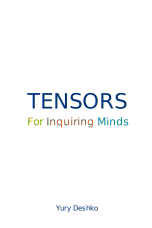
\includegraphics[width=\paperwidth]{pics/bookCoverInner_Var1}}; % Background image
%\draw[anchor=north] (midpoint) node [fill=ocre!30!white,fill opacity=0.6,text opacity=1,inner sep=1cm]{\Huge\centering\bfseries\sffamily\parbox[c][][t]{\paperwidth}{\centering Relativity\\[15pt] % Book title
%{\Large For the Inquiring Mind}\\[20pt] % Subtitle
%{\huge Dr. Yury Deshko}}}; % Author name
\end{tikzpicture}};
\end{tikzpicture}
\vfill
\endgroup
\newpage

%----------------------------------------------------------------------------------------
%	COPYRIGHT PAGE
%----------------------------------------------------------------------------------------

~\vfill
\thispagestyle{empty}
\phantom{x}\\
Quantum Physics At Any Cost\\
Yury Deshko \textsc{www.srelim.com}\\
ISBN 978-1-7948-2018-0\\
\begin{figure}[htbp]
  %\centering
  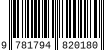
\includegraphics[scale=1.0]{pics/ISBN_978_1_7948_2018_0}
\end{figure}
\noindent Copyright \copyright\ \the\year{}  \noindent\\ % Copyright
All rights reserved.\\
Imprint: Lulu.com


%\noindent Licensed under the Creative Commons
%Attribution-NonCommercial 3.0 Unported License (the ``License''). You
%may not use this file except in compliance with the License. You may
%obtain a copy of the License at
%\url{http://creativecommons.org/licenses/by-nc/3.0}. Unless required
%by applicable law or agreed to in writing, software distributed under
%the License is distributed on an \textsc{``as is'' basis, without
%  warranties or conditions of any kind}, either express or
%implied. See the License for the specific language governing
%permissions and limitations under the License.\\ % License information
%
%\noindent \textit{First printing, March 2017} % Printing/edition date
\newpage
%----------------------------------------------------------------------------------------
%	DEDICATION PAGE
%----------------------------------------------------------------------------------------

\begingroup
\thispagestyle{empty}
\begin{tikzpicture}[remember picture,overlay]
\coordinate [below=12cm] (midpoint) at (current page.north);
\node at (current page.north west)
{\begin{tikzpicture}[remember picture,overlay]
\node[anchor=north west,inner sep=0pt] at (0,0) {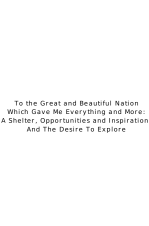
\includegraphics[width=\paperwidth]{pics/dedication}}; % Background image
%\draw[anchor=north] (midpoint) node [fill=ocre!30!white,fill opacity=0.6,text opacity=1,inner sep=1cm]{\Huge\centering\bfseries\sffamily\parbox[c][][t]{\paperwidth}{\centering Relativity\\[15pt] % Book title
%{\Large For the Inquiring Mind}\\[20pt] % Subtitle
%{\huge Dr. Yury Deshko}}}; % Author name
\end{tikzpicture}};
\end{tikzpicture}
\vfill
\endgroup
\newpage



%----------------------------------------------------------------------------------------
%	TABLE OF CONTENTS
%----------------------------------------------------------------------------------------

%\usechapterimagefalse % If you don't want to include a chapter image, use this to toggle images off - it can be enabled later with \usechapterimagetrue

\chapterimage{pics/chapterImageDefault.pdf} % Table of contents heading image

\pagestyle{empty} % No headers

\tableofcontents % Print the table of contents itself

\cleardoublepage % Forces the first chapter to start on an odd page so it's on the right

\pagestyle{fancy} % Print headers again



%----------------------------------------------------------------------------------------
%	PART
%----------------------------------------------------------------------------------------
\section*{Acknowledgment}
My sincere gratitude goes to all reviewers of the early drafts of
the book for their valuable feedback. In particular, I want to thank Dr. Alex
Rylyakov, Dr. Mikhail Makouski, Prof. Anton Kananovich,
and Dr. Mohammad Teimourpour. To Dr. Teimourpour I must give separate
thanks for numerous discussions, helpful suggestions on material
presentation, and hospitality.

\emph{My friends, discussing the book with you was both illuminating
and fun.}

Finally, special acknowledgment must be given to my son, Daniel, for
his help with fixing colors in many figures.

\begin{flushright}
  \begin{tabular}{@{}l@{}}
    Yury Deshko\\
    Weehawken, New Jersey\\
    2024
  \end{tabular}
\end{flushright}


\chapter*{Preface}
\chapterimage{pics/chapterImageDefault.pdf}
This book is the result of lectures delivered to curious, motivated, and studious high schoolers. The lectures ran  during the years 2019-2024 in various formats, but mostly in class during a three week summer school organized by Columbia University Pre-College Programs. Additionally, the same lectures were taught remotely to selected students of Ukrainian Physics and Mathematics Lyceum. 

The material has been designed to be accessible to people with solid background in high-school algebra and physics (mostly mechanics). Several years of teaching to a relatively diverse set of students proved that nearly all material can be efficiently absorbed by most, provided diligent work is done on exercises and problem. The last fact confirms a well-known truism: \emph{No real learning occurs without practice.}

Exercises are essential part of this book.  They are carefully selected to help readers get better understanding of the material and they are also fully solved. The difficulty of the exercises varies from simple to quite challenging.

This book \emph{is not a standard textbook}. It lacks the breadth and rigor present in many excellent introductions into Quantum Physics. The best way to view this book is as a \emph{bridge} between  elementary and popular books and the more challenging college-level textbooks. 

Although the topic of the book is mathematical, the exploration will
lack proper mathematical rigor, aiming instead at simplicity, clarity,
and the use of helpful analogies.

This book is {\bf not intended} to substitute more serious textbooks on linear
algebra or tensor algebra. Hopefully, the main benefit of
reading this book -- either before, or after, or in addition to other
books on the subject -- is that it should help lower the
\emph{``mental barrier''}\index{Barrier!mental} we all encounter when
learning new concepts, especially abstract mathematical concepts.

To comprehend and enjoy the material of this book the reader should
have a solid knowledge of basic high-school algebra and an open and
inquiring mind. The book is a bit longer that it could have been
because all derivations are detailed and all exercises are fully
solved.

Some sections are marked with an asterisk, for example
{\bf Transposition*}. Those sections contain material that is either
optional or a bit more advanced that usual. These sections can be
skipped without significant impact on the main message of the book.


\section*{At Any Cost}
The subtitle of this book has been inspired by the letter written by Max Karl Ernst Ludwig Planck to an American physicist



%\part{Part 1: Fun}
%
\chapterimage{pics/chapterImageIntroduction.pdf}
%\chapterimage{introduction.pdf}
\graphicspath{{../01Introduction/pics/}}

\chapter{Introduction}\label{ch:Introduction}

\begin{quoting}
	This quantum business is so incredibly important and difficult that everyone should busy himself with it. 
	
	
	A. Einstein in a letter to his friend Jakob Laub in 1908, as quoted by A. Wheeler in “The Mystery and The Message Of The Quantum”
\end{quoting}

{\bf Abstract}\hspace{0.2cm} In this chapter.


\lettrine[lines=2]{\color{darkocre}Q}{uantum physics is a century-old branch of physics. Its success} is unparalleled and yet quantum physics is unfinished in one sense: There is no clear and widely adopted consensus on what some of quantum ideas "really mean."

\section{What Is Quantum Physics?}
There are many characterizations of quantum physics.  In essence, quantum physics is the part of physics which focuses on \emph{quantum systems} -- physical systems showing \emph{quantum behavior}. So, what effects or phenomena are quantum?


\section{Brief Historical Context}
The year 1900 is usually considered the birth year of quantum physics. On December 14 of 1900, at the meeting ????, the German physicist Max Karl Ernst Ludwig Planck presented his theoretical explanation of the \emph{spectrum} of electromagnetic radiation emitted by hot bodies. In his work he introduced what is now known as \emph{Planck's constant}  $h$, which has a physical meaning of \emph{elementary quantum of action}.
\begin{mybio}{Niels Bohr On $h$}
	The Danish physicist Niels Bohr, one of the founders of quantum physics, wrote: 
	
	\emph{
	"A new epoch in physical science was inaugurated, however, by Planck’s discovery of the elementary quantum of action, which revealed a feature of wholeness inherent in atomic processes, going far beyond the ancient idea of the limited divisibility of matter."
}
	
	(Atomics Physics and Human Knowledge, Quantum Physics and Philosopy, Complimentarity and Causality.)
\end{mybio}
Let's take a look at what happened before and after Planck's discovery.

\subsubsection*{Pre-History: Spectroscopy and Molecular Theory}
The evolution of physics in the century preceding quantum era is fascinating. It is important to know some of pre-history in order to appreciate the context in which quantum physics was born. We will highlight two big advancements, one in experimental, and the other in theoretical departments. 

\subsubsection*{Spectroscopy}
First, the methods of \emph{spectroscopy}--study of energy distribution across various wavelengths of visible and invisible light--experienced significant development. Already in 1802 an English chemist and physicist William Hyde Wollaston observed that\footnote{Wollaston William Hyde 1802 XII. \emph{A method of examining refractive and dispersive powers, by prismatic reflection}, Phil. Trans. R. Soc. {\bf 92}: 365–380 } "If a beam of day-light be admitted into a dark room by a crevice 1/20 of inch broad\footnote{1/20 in = 1.27 mm.}, and received by the eye at the distance of 10 or 12 feet\footnote{10-12 feet = 3-3.7 m.}, through a prism of flint glass" one can see four colors (red, yellowish green, blue, and violet) separated by \emph{dark lines}. Soon many more dark lines in the optical spectrum of the Sun were discovered and systematically studied by a German physicist Joseph Ritter von Fraunhofer. Today these \emph{Fraunhofer lines} are understood to result from the \emph{absorption} of radiation by different atoms in the atmospheres of the Sun and earth.
\begin{figure}[htbp]
	\centering
	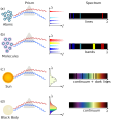
\includegraphics[scale=1.0]{spectraTypes}
	\caption{Various types of spectra observed from different substances. (a); (b); (c); (d). See text for explanation.}
	\label{fig:spectraTypes}
\end{figure}


The energy absorbed by a substance can be \emph{emitted}. The study of \emph{emission spectra} from various bodies revealed a great deal of complexity and provided a lot of information about bodies' material composition and state. 

There are four basic types of spectra one can observe, as illustrated in Figure \ref{fig:spectraTypes}. In a typical spectroscopic observation radiation from an excited object is sent through a \emph{dispersive} component, such as a prism or a diffraction grating\footnote{See Visual Glossary}. A beam of radiation is spread out according to colors and light of different color falls at different place of a detector (eye, photographic plate, or an electronic camera).

Light emitted by atoms consists of very definite colors which show up as \emph{emission lines} in spectra, as shown in Figure \ref{fig:spectraTypes}(a). Exact locations of such lines tell which atom emits the radiation. Simpler atoms, such as hydrogen or helium, have simpler spectra.

Spectra of excited molecules contain many closely placed lines. Sometimes multiple lines coalesce into a \emph{band}, as in Figure \ref{fig:spectraTypes}(b).

Radiation from large hot bodies, like Sun, reveals both discrete and continuous color distribution; see Figure \ref{fig:spectraTypes}(c). All colors are present in the spectrum, and dark Fraunhofer lines indicate that some of the radiation has been absorbed on its way to the detector by atoms and molecules.

Finally, an important radiation type corresponds to an \emph{idealized} object, called \emph{black body} -- a theoretical material which does not relfect any incident radiation. In other words, \emph{black body absorbs all incoming radiation}. Of course, black body also emits radiation, otherwise it would never stop accumulating energy from incident light. Therefore, black body \emph{is not truly black}, its perceived color depends on the temperature of the body. Emission spectrum of black-body, called \emph{black body radiation} or \emph{normal spectrum}, is of great interest, because it approximates emission spectrum from \emph{any material} kept at a constant temperature.
At the end of the 19th century, black body radiation was actively studied both experimentally and theoretically. 

\begin{mybio}{Max Planck And Black Body Radiation}
	Since black-body radiation spectrum does not depend on particular material, it has a universal nature. This fascinated Max Planck, as he wrote in his Scientific Autobiography\footnote{Max Planck, \emph{Scientific Autobiography and Other Papers}, Williams \& Norgate, 1950, pp. 34-35.}:
	
	\emph{"Thus, this so-called Normal Spectral Energy Distribution represents something absolute, and since I had always regarded the search for the absolute as the lofties goal of all scientific activity, I eagerly set to work."}
	
	\[
	\delta E = \rho\delta \nu = \frac{8\pi h\nu^3\delta\nu}{c^3}\frac{1}{e^{h\nu/kT}-1}\,.
	\]
\end{mybio}

The spectrum of black body radiation was the first type of spectrum to receive a theoretical explanation and an explicit formula. Spectra of atoms and molecules were properly studied only after the development of quantum mechanics.

Spectroscopy of the 19th century\footnote{William McGucken, \emph{Nineteenth-Century Spectroscopy}, The Johns Hopkins Press, 1969.}

\subsubsection*{Molecular Theory}
Second advancement of pre-quantum physics was connected with the hypothesis of atoms and molecules. Although atomistic ideas had been known for about two millenia, even in the 19th century far from every physicist was convinced that atoms and molecules were objects just as real as everyday things. There was no \emph{direct evidence} for the existence of atoms and molecules, and the main support for the atomistic views came from \emph{indirect evidence}, like the many useful results that followed from molecular theory. For example, the behavior of gases (diffusion, viscosity, laws connecting pressure and temperature, heat capacity, etc.) was especially well explained. Two major figures in this field were the Scottish physicis James Clerk Maxwell and the German physicist Ludwig Boltzmann.

In September of 1899, at the congress of the German Society of Natural Scientists and Physicians,  Ludwig Boltzmann presented a review titled \emph{"The Recent Development of Method In Theoretical Physics."}\footnote{\emph{The Monist}, January, 1901, Vol. {\bf 11}, No. 2, pp. 226-257.} He highlighted the rapid development of physics in the 19th century and discussed major experimental and theoretical results.

\begin{mybio}{Boltzmann's Prediction}
	\emph{"I have to mention finally the relations which obtain according to the molecular theory between the principle of entropy and the calculus of probabilies, concerning the real significance of which there may be some difference of opinion, but which, no unprejudiced person will deny, are eminently qualify to extend our intellectual horizon and to suggest new combinations both of ideas and experiments."}
\end{mybio}
Boltzmann's anticipation that "the principle of entropy and the calculus of probabilities" will lead to "new combinations both of ideas and experiments" was fully confirmed by Max Planck in about a year!

As explained in the Section XX, Max Planck used nearly the same approach as Boltzmann to calculate entropy of a thermodynamic system. Only in his case, the system was not an ideal gas of molecules, but a collection of oscillating molecules that interact with electromagnetic radiation (in the form of heat).


\subsection{Three Ages of Quantum}
The evolution of quantum science and technology can be roughly divided into three stages: (a) "Old quantum physics" (b) modern quantum physics, and (c) information-age quantum physics (see Figure \ref{fig:quantumTechnologyEvolution}).
\begin{figure}[htbp]
	\centering
	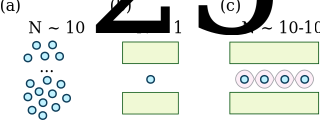
\includegraphics[scale=1.0]{quantumTechnologyEvolution}
	\caption{Three stages of quantum science and technology: (a) Observation of large groups of objects (atoms, molecules); (b) Study of interaction between single particles (one atom + one photon); (c) Connecting tens and hundreds of quantum systems using \emph{entanglement}.}
	\label{fig:quantumTechnologyEvolution}
\end{figure}



\subsubsection*{Old Quantum Physics}

\subsubsection*{Modern Quantum Physics}

\subsubsection*{Information Age}


\section{Who Needs Quantum Physics?}

In October of 1912, Albert Einstein\index{Einstein} wrote in a letter to his physicist
friend Arnold Sommerfeld:
\begin{mybio}{Example of mybio environment}
  I am now exclusively occupied with the problem of gravitation theory
and hope, with the help of a local mathematician friend, to overcome
all the difficulties. One thing is certain, however, that never in my
life have I been quite so tormented. A great respect for mathematics
has been instilled within me, the subtler aspects of which, in my stupidity,
I regarded until now as a pure luxury. Against this problem [of
  gravitation] the original problem of the theory of relativity is
child’s play.
\end{mybio}
In the period from 1905 to 1916 Einstein was feverishly working on the
General Theory of Relativity\index{General relativity} -- the next
best theory of gravity since
Newton. The mathematics of general relativity is based on the calculus
of tensors, created by Italian mathematicians Ricci-Curbastro and
Levi-Civita roughly a decade before Einstein started working on the
problem of gravity.


\section{Why is Quantum Physics Hard?}\label{sec:WhyQuantumHard}
Quantum physics is not an easy subject.  Mastering it requires learning new physical concepts and advanced mathematical tools. Additionally, it is necessary to examine critically some basic intuitive notions of classical physics and everyday experience.  All this takes time and effort.

\begin{mybio}{Feynman on Quantum Physics}
	In his book {\it The Meaning of It All}, Richard Feynman -- an American theoretical physicist and Nobel laureate -- wrote:
	
	
	"Trying to understand the way nature works involves a most terrible test of human
	reasoning ability. It involves subtle trickery, beautiful tightropes of logic on which one
	has to walk in order not to make a mistake in predicting what will happen. The quantum
	mechanical and the relativity ideas are examples of this."
	
	
	{\it The Meaning of It All, Section I: The Uncertainty of Science.}
\end{mybio}

Let us examine those features of quantum physics that make it particularly challenging and discuss what can be done to make the learning easier.

\subsection{Indirect Experience}
Concepts of classical physics, especially when applied to macroscopic objects, can often be connected to our experiences. Velocity, heat, force, pressure, motion of projectiles, currents of fluids, propagation of sound and so on -- all can be felt, seen, or otherwise perceived by humans. In contast, \emph{we do not have a direct access to the quantum side of the world.}  There are no experiments where one can say "Here, look at this entanglement!" or "Hey, touch this quantum of action!", or "Listen carefully, that is the decoherence!"

\begin{analogy}
	Imagine you want to understand the life of inhabitants of extremely distant land. The environment and climate of that land makes it impossible for you to travel there and see everything with your own eyes. 
	
	Who knows, maybe they do not have such notions as "home", "road", "tomorrow", "force", and so on.
	
	Now, if by "understand" we mean "explain and predict the behavior of aliens in our own terms", then the task might be hopeless. However, if by "understand" we mean "develop new concepts that describe and predict the behavior of aliens" then we might have a chance. Of course, the new concepts might be very foreign to us, at first. But the more we use them -- the less our mind struggles.
\end{analogy}


The problem then becomes two-fold. First, we need give up our non-quantum intution. Remember, our intution and conceptual pictures are rooted in macroscopic reality. We interact with the latter using our macroscopic organs and instruments which are unable to capture subtle non-classical features of the world. 

Second, we need to develop new intution and set of "pictures"/models which would be adequate for quantum world. While doing so, we must be careful not to "contaminate" this new way of thinking with old concepts. 

\subsection{Abstract Mathematics}
The mathematics used in modern physics is becoming increasingly more abstract. It is the price to pay for the powerful and general tools which are indespensible for expressing most advanced results of physics, either  classical or quantum.

Quantum physics does not use any special mathematical methods which would make it more challenging than classical physics. Of course, a student learning quantum theory might struggle with the heavy use of operators, complex vectors,  Hilbert spaces, commutators, matrices and so on. The difficulty, however, is not due to the quantum nature of the subject, since nearly all these mathematical concepts and tools could be found in other -- non-quantum -- areas of mathematical physics.

\begin{mybio}{Alfred Whitehead on Abstract Mathematics}
	Nothing is more impressive than the fact that as mathematics withdrew increasingly into the upper regions of ever greater extremes of abstract thought, it returned back to earth with a corresponding growth of importance for the analysis of concrete fact. ...The paradox is now fully established that the utmost abstractions are the true weapons with which to control our thought of concrete fact
	
	{\it Mathematics as an Element in the History of Thought, Ch. 2, p. 46}
\end{mybio}

Surprisingly, current mathematical framework of quantum physics is the simplest possible. Quantum theory is \emph{linear}, meaning that it is based on the \emph{superposition principle} and uses the \emph{simplest} kinds of operators -- \emph{linear operators}. It must be noted that the linearity is not exclusive to quantum theory, as, for example,  classical electrodynamics is also a linear theory.


\subsection{Inadequate Language}
Perhaps the biggest barrier on the path to mastering quantum physics is... \emph{ordinary language}. It has developed to communicate everyday experiences and emotions, but subtle natural phenomena are far removed from either of those.

\begin{mybio}{Bertrand Russell On Ordinary Language}
Ordinary language is totally unsuited for expressing what physics really asserts, since the words of everyday life are not sufficiently abstract. Only mathematics and mathematical logic can say as little as the physicist means to say.

{\it The Scientific Outlook (1931)}
\end{mybio}

\begin{mybio}{Werner Heisenberg On Ordinary Language}
	It is not surprising that our language should be incapable of describing the processes occurring within the atoms, for, as has been remarked, it was invented to describe the experiences of daily life, and these consist only of processes involving exceedingly large numbers of atoms. Furthermore, it is very difficult to modify our language so that it will be able to describe these atomic processes, for words can only describe things of which we can form mental pictures, and this ability, too, is a result of daily experience.
	
	{\it Principle of Quantum Theory (1930), Introductory, p. 11}
\end{mybio}
 
To capture deep and nuanced laws of nature, we must use a language of adequate power, built with new words and symbols completely foreign to common intuition and simple mental pictures. In other words, the adequate language has to be \emph{abstract}, \emph{purposefully developed}, and most likely \emph{unintuitive} to an untrained mind.
 
\begin{remark}
	Constructing new languages is a standard task in the field of computer science. New languages are regularly proposed to better describe computational tasks in a specific domain. For example, a separate language exists for working with database requests.
	
	In this field, a \emph{domain specific language} is usually developed to address problems 
	
	A language is considered good if it does not allow constructing meaningless or harmful statements. For example, if a language allows definition of a set of sets which are not elements of themselves, the this language will be plagued with the famous Russell paradox.  
	
	Natural human language is notoriously bad for formulating precise and abstract results of science.
\end{remark}

\begin{myrem}{Particles}
	Particles are excitations of quantum fields. They correspond to irreducible unitary representations of Lorentz group. Fields are operator-valued vector functions defined over Minkowski space and transformed simply under the action of the Poincare group.
\end{myrem}
Learning this language is the key to success. 

\section{Quantum Versus Classical}
When do we have to use quantum physics? Where is the border between quantum and classical phenomena?

\begin{figure}[htbp]
  \centering
  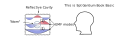
\includegraphics[scale=1.0]{defaultFigureTemplate}
  \caption{Diagrams are used to graphically represent sets of objects
    and relationships between them. Arrows can connect (map) elements
    of one set with another. Such mappings may have names: {\bf mlg}
    returns mileage for a given car, {\bf clr} -- color, and {\bf smk}
  determines whether two cars are of the same make.}
  \label{fig:diagrams}
\end{figure}


\section{Quantum Enigma}
There are many adjectives that can be applied to quantum physics. It is tremendously successful, impactful,  fascinating, and intellectually rewarding. It also appears to be the "least understood" part of physics.

\begin{mybio}{What is Quantum Mechanics?}
	In 1968 in a German town Lindau, 480 young scientists met with 20 Nobel Laureates in Physics  -- the founders and major contributors to quantum physics. By this time the theory of quantum physics was fully formulated and applied to many important problems. One of the paticipating Nobel Laureates -- Willis E. Lamb Jr -- wrote:
	
	"A remarkable feature of the 1968 conference of Nobel prize winners in physics at Lindau is that it was possible for me to ask such question in the presence of two of the founders of quantuam mechancis, Werner Heisenberg and P. A. M. Dirac, more than 30 years after the discovery, in a lecture attended by 400 students who had recently begun their study of the subject." 
\end{mybio}

By 1968 nearly all fundamental papers and  many great textbooks on quantum physics had been written, including the books by the founders of quantum mechanics. Didn't those works define what quantum mechanics was?

By now quantum physics has demonstrated even greater success. And yet the question "What is Quantum Mechanics?" is still routinely asked in many books and articles. We are still puzzled by this enigmatic omni-tool that we discovered.


There are many challenges still.

"In summary, in the span of less than two decades, photonic quantum information science has matured immensely. [...]. The number of photons simultaneously used in experiments has grown, from 2 to 4 up to 12"
(Appl. Phys. Rev. 6, 041303 (2019); doi: 10.1063/1.5115814)


\begin{figure}[htbp]
  \centering
  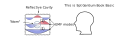
\includegraphics[scale=1.0]{defaultFigureTemplate}
  \caption{Schematics can be used to represent functions, operators,
    their compositions and structure.}
  \label{fig:schematicExample}
\end{figure}


\

\vspace{1cm}
\section*{Chapter Highlights}
{\setstretch{1.5}\chhc
  \it
\begin{itemize}
\item Natural evolution of mathematical objects from numbers, through
  vectors, leads to tensors.
\item Each successive tier of mathematical object in the progression
  ``numbers, vectors, tensors''  is more abstract and more powerful.
\item Numbers, vectors, and tensors are all conceptually connected.
\end{itemize}
}

%
%
%
\chapterimage{pics/chapterImageNumbers.pdf}
%\chapterimage{geometry.pdf}
\graphicspath{{../02Physics/pics/}}
	
\chapter[Physics]{Physics}\label{ch:Physics}

\lettrine[lines=2]{\color{darkocre}N}{umbers} are powerful
mathematical objects. They are used to solve
an endless list of problems that involve \emph{quantities}. As
mathematics
and sciences progressed, natural numbers evolved into whole
numbers, then into rational numbers and beyond.\footnote{A superb account of
this process is given in the book \emph{``Number: The Language of
Science''} by Tobias Dantzig.}

\begin{myprereq}{Prerequisite Knowledge}
	To fully understand the material of this chapter, readers should be comfortable with the following concepts:
	
	\begin{itemize}
		\item \phantom{phantom}
		\vspace{-0.5cm}
		\item State
		\item Dynamical equations
	\end{itemize}	
\end{myprereq}

\section{Goals and Methods}
Physics is a \emph{human} activity pursuing the following major goals: \emph{Describe}, \emph{explain}, and \emph{predict} phenomena comprising the observed world.

results can be applied in a wide range of fields. In part, the universality of mathematics
stems from the \emph{general} and \emph{abstract} nature of mathematical
concepts. Let us illustrate this using an example.

\begin{SCfigure}%[htbp]
  %\centering
  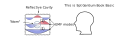
\includegraphics[scale=1.0]{defaultFigureTemplate}
  \caption{49 objects can be arranged in a square 7x7. 48 objects can
    be arranged as a rectangle of 6x8.}
  \label{fig:numbersExampleGenerality}
\end{SCfigure}

An astute farmer notices that 49 sacks of grains can be arranged
in a square with each side having 7 sacks (see the Figure
\ref{fig:numbersExampleGenerality}). When one sack is used up, the
remaining 48 sacks can be arranged as a rectangle 6 by 8 sacks.


\begin{exercise}\label{exe:relationsGeneral}
Think how you would represent the generalized relations of the types
given in the Figure \ref{fig:schematicRelationNtoN} at the level of
sets? What kind of diagrams would you draw?
\end{exercise}

\section{Common Sense}
Mathematics is a remarkably effective and universal discipline, its
methods and
results can be applied in a wide range of fields.
\subsection{Detached Observer}
\begin{figure}[htbp]
	\centering
	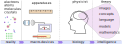
\includegraphics[scale=1.0]{commonSensePerception}
	\caption{Observer in classical view of the world is detached, separated from the "true" reality.}
	\label{fig:commonSensePerception}
\end{figure}


\section{Deterministic Evolution}
The completeness of a state is a very strong constraint. Not only it means "everything there is to know at a given moment", but also "know state now -- know state always." The latter is an expression of \emph{determinism}: the knowledge of a system is completely determined once the state and its law of evolution are known.

  However, state by itself  is not sufficient to satisfy the latter requirement, it must be supplemented by the so called \emph{dynamical equations}. These equations are specific to a physical system and encapsulate the laws that govern internal interactions. EXAMPLE?

Denoting the mathematical representation of the state as $\xi$, the evolution of the state between the moments of time $T=t$ and $T=\tau$ may be written as a functional dependence:
\[
\xi_\tau = U_{\tau, t}\,\xi_t\,.
\]
For $\tau > t$ we determine the future state, while for $\tau < t$ we determine the state in the past (relative to the moment $t$).
\begin{myExample}
	For circular motion the state is the angle $\xi=\phi$, and the evolution is given by a simple formula
	\[
	\phi_\tau = U_{\tau, t}\,\phi_t=\omega (\tau - t) + \phi_t\,.	
	\]
	Notice that in this case the evolution function depends on the time \emph{difference} $\tau-t$ and not on each moment of time separately:
	\[
	U_{\tau, t} = U_{\tau-t}\,.
	\]
\end{myExample}
It must be emphasized again, that the final state $\xi_f=\xi_\tau$ is determined by two factors: the initial state $\xi_i=\xi_t$ and the laws of physics encoded in the evolution function $U_{\tau, t}$. 

\begin{figure}[htbp]
	\centering
	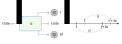
\includegraphics[scale=1.0]{evolutionOperatorBox}
	\caption{Evolution operator transforms an initial state into the final state in time $\Delta t$.}
	\label{fig:evolutionOperatorBox}
\end{figure}

The laws of physics are timeless\footnote{Technical term is \emph{time-translation invariant.}}, as illustrated by the Coulomb's law of interaction between charges $q$ and $Q$ at a distance $r$ apart: $F_C=k qQ/r^2$. The timeless nature of the physical laws requires that the same initial state $\xi_i$ evolves into the same final state $\xi_f$ regardless of when the evolution starts and as long as the time interval between the beginning and the end of evolution is the same. Mathematically this is expressed as follows:
\[
U_{\tau, t}\,\xi_i  = U_{\tau', t'}\,\xi_i
\]
for \emph{any} initial state $\xi_i$, as long as $\tau'-t'=\tau-t=\Delta t$.

Thus, for \emph{any} values of $t$ and $t'$, we have
\[
U_{t+\Delta t, t}  = U_{t'+\Delta t, t'}\,.
\]
This equation says that the evolution function $U$ becomes insensitive to the values $t$ and $t'$, and only depends on $\Delta t$ -- the time interval between the beginning and the end of evolution. Therefore, we can write the following connection between the states at different moments:
\[
\xi_{t+\Delta t} = U_{\Delta t}\,\xi_t\,.
\]
This connection holds \emph{for any moment of time} $t$ and time interval $\Delta t$.

In physics the states are represented using numbers, vectors, functions, and similar mathematical objects. Common to all of these types of objects is a very basic property of "additivity" and "scalability". That is, one can -- at least formally -- add and subtract states, as well as multiply them by numbers. For example, for any two states $\xi_1$ and $\xi_2$, one can write  equations like
\[
\xi_3 = 2\xi_1 + 3\xi_2\qquad\textrm{ or }\qquad \Delta \xi = \xi_2 - \xi_1\,.
\]

Depending on a particular representation of the state, the evolution function $U$ might be a "usual" function, an operator, or something else entirely. Regardless of what the exact \emph{type} of $U$ is, its job is always the same -- map initial state $\xi_i$ at time $t$ into the final state $\xi_f$ at time $t+\Delta t$.
 
For $\Delta t = 0$ the evolution function $U$ must be a simple \emph{identity} function:
\[
U_0 = I\,.
\]
Furthermore, for a continuous evolution, it is necessary for small changes in time $\delta t$ to produce small changes in the state $\delta \xi$:
\[
\xi_{t+\delta t} = U_{\delta t} \xi_t = \xi_t + \delta \xi\,.
\] 
For a continuous evolution of the state, the evolution function $U$ must be continuous. This implies that for small time intervals it produces small changes:
\[
U_{\delta t} \approx I + \delta U = I + G\delta t\,,
\]
where $G$ is called the \emph{generator} of state evolution. The meaning of the generator is clear from its definition -- it specifies how fast the state evolution happens: $G=\partial_t U$.

In terms of the generator, the evolution equation can be written using the relations 
\[
\delta \xi = \xi_{t+\delta t} - \xi_t = \left(I + G\delta t\right)\xi_t - \xi_t = G\delta t\xi_t\,.
\]
Finally, dividing both sides by $\delta t$ and using the $\partial$-notation, we arrive at the Schrodinger-type of equation for the \emph{continuous} state evolution:
\begin{equation}
	\partial_t \xi = G\,\xi_t\,.
	\label{eq:SchrodingerTypeEq}
\end{equation}
The equation (\ref{eq:SchrodingerTypeEq}) is a general form of state evolution equations used in physics. It appears in many cases where the dynamics of a system is described as a \emph{continuous deterministic evolution}. 
\begin{mybio}{Deterministic Evolution Equations}
	Equations similar to (\ref{eq:SchrodingerTypeEq}) can be found in many physical theories. In quantum theory it is Schrodinger equation, which can be written as follows:
	\[
	\partial_t\ket{\Psi} = -i\hat{H}\,\ket{\Psi}\,.
	\]
\end{mybio}


\section{Classical and Quantum}
Mathematics is a remarkably effective and universal discipline, its
methods and
results can be applied in a wide range of fields.

\section{State}
State is a very important concept in physics. It means \emph{complete} but \emph{minimal} knowledge about  possible behavior of a given system.
\begin{figure}[htbp]
	\centering
	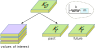
\includegraphics[scale=1.0]{stateAsKnowledge}
	\caption{State is a minimal and complete knowledge about a physical system.}
	\label{fig:stateAsKnowledge}
\end{figure}
By \emph{minimal} knowledge we mean that if position of particle $x$ is known, there is no need to know $x^3$ or any other one-to-one function of position. We only need to know and keep track of the \emph{essential} information.


\section{Measurement}
Measurement is the source of our knowledge about the world. This is true for both classical and quantum physics. 
\begin{figure}[htbp]
	\centering
	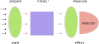
\includegraphics[scale=1.0]{measurementStages}
	\caption{Three stages of measurement process: Preparation of a system in a certain state, followed by the interaction of the system with external system, ending with the measurement which extract the information.}
	\label{fig:measurementStages}
\end{figure}

\section{Atoms}
Classical physics predicts a continuous decay of unstable configuration of charges. What is observed is a spontaneous decay of stable configuration of charges. Quantum physics elegantly explains the latter.  

\section{Particles}
Classical physics predicts a continuous decay of unstable configuration of charges. What is observed is a spontaneous decay of stable configuration of charges. Quantum physics elegantly explains the latter.  

\section{Polarization and Spin}
Mathematics is a remarkably effective and universal discipline, its
methods and
results can be applied in a wide range of fields.

% ---------------------- Chapter Highlights -------------------------------
\section*{Chapter Highlights}
{\setstretch{1.5}\chhc
  \it  
\begin{itemize}
\item The power of mathematical concepts and methods increases with
  the level of abstraction.
\item Learning new concepts often involves learning new
  terminology. The latter can create an artificial mental barrier.
\item ``Usual'' numbers form a mathematical structure. The structure
  is revealed through various relations that exist between numbers.
\item Relations between numbers are expressed using the concept of
  functions and operations (e.g., addition). Each operation is
  characterized by its arity -- the number of arguments it accepts as
  an input.
\end{itemize}


}

%
%
%
\chapterimage{pics/chapterImageArrows.pdf}
%\chapterimage{spacetime.pdf}
\graphicspath{{../03Mathematics/pics/}}

\chapter{Mathematics}\label{ch:Mathematics}

\lettrine[lines=2]{\color{darkocre}M}{athematical concepts and tools used in quantum theory are} not significantly different from the ones used in classical physics. This fact, of course, does not make them any easier, but it is important to remember that there is no special mathematics that makes quantum physics extra challenging.

In this chapter we develop mathematical tools needed for quantum theory. This is an essential investment that will pay off when we start discussing quantum phenomena. Mathematics plays a vital role in quantum physics since it becomes the only guide in the field where intuition and simple mental pictures fail.

\begin{myprereq}{Prerequisite Knowledge}
	To fully understand the material of this chapter, readers should be comfortable with the following concepts:
	
	\begin{itemize}
		\item \phantom{phantom}
		\vspace{-0.5cm}
		\item State
		\item Dynamical equations
	\end{itemize}	
\end{myprereq}


\section{Randomness}
Randomness is the opposite of certainty, \emph{determinism}, and complete predictability. Randomness (or \emph{indeterminism}) plays an essential part in quantum physics.

Mathematical description of randomness is based on the idea of \emph{probability}. Probability quantifies (measures) the qualitative notion of \emph{likelyhood} of certain outcomes. A common example is the toss of a coin where the probability of tail is $1/2$, or the throw of a dice, where the probability of getting a face value divisable by 3 is $1/3$.

In quantum physics probability of an event $E$ happening is understood as the \emph{relative frequency} or ratio of the number of occurences of the given event in $N$ trials:
\[
P_E = \frac{N_E}{N}\,,
\]
where $P_E$ is the probability of the event $E$, and $N_E$ is the number of times the event happens during an experiment.

For example, suppose  we are measuring a week light with a detector capable of detecting  single photons. An arriving photon triggers the detector which produces a pulsed electronic signal, like a spike in the output voltage.

Denoting $N$ the number of times the detector is triggered during an experiment. If $N_A$ is the number the detector $A$ is fired, then the probability of detecting a signal there is 
\[
P_A = \frac{N_A}{N}\,.
\]
?$N_A + N_B$ if both are working?


\subsection{Schrodinger Student}
In 1935 paper discussing quantum features, such as \emph{entanglement}, Erwin Schrodinger introduced his famous cat. He also discussed an example of students.


\section{Functions}

The idea of a function is a very basic one. Essentially, function is an unambiguous \emph{rule}, an \emph{algorithm}, which associates a certain value $y$ (\emph{result} or \emph{output} of a function) with every meaningful \emph{input} value $x$ (\emph{argument} of a function). As an example, consider the following  function:
\[
y=\frac{1}{2x^2+5}\,.
\]
For any real number $x$ we can compute the value $y$ using only basic arithmetic operations. 

Next consider a function $\btc{sqrt}$ which computes a square root of a number: $y=\btc{sqrt}\,x$. If we only work with real numbers, the range of meaningful inputs is reduced -- only non-negative input values $x$ are allowed. Another thing to notice is that now the function is simply given a name  $\btc{sqrt}$  and shows no structure -- it is not expressed in terms of other more basic operations. A few important functions are given names: 
$\sin\,,\cos\,,\exp\,,\log\,,\btc{abs}$\footnote{Absolute value of a number -- its positive magnitude.} and several more. Of course, the square root of a number is traditionally written with a special sign -- called a \emph{surd}: $\btc{sqrt}\,x=\sqrt{x}$.

\subsection{Function Boxes}
The input-output view of functions leads to a helpful picture where a given function is represented as a box with an input and an output (or multiple inputs and even multiple outputs), as illustrated in Figure \ref{fig:functionAsBox}.
\begin{figure}[htbp]
	\centering
	\includegraphics[scale=1.0]{functionAsBox}
	\caption{A function can be viewed as a box with input(s) and output(s).}
	\label{fig:functionAsBox}
\end{figure}


\begin{figure}[htbp]
	\centering
	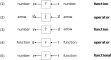
\includegraphics[scale=1.0]{functionTypes}
	\caption{Several types of functions: (1); (2); (3); (4); (5).}
	\label{fig:functionTypes}
\end{figure}

\subsection{Application Notation}
The dominant rule for writing function $f$ applied to an argument $x$ uses parentheses around the argument, like so: $f(x)$. This rule, however, is \emph{not absolute} and is abandoned as soon as one uses functions in linear algebra. For example, when an operator $\op{f}$ is applied to a vector $\ket{x}$, we would write $\op{f}\,\ket{x}$, without the parentheses. 

In this book we will use a uniform rule for function application: \emph{Function and its argument are separated by a space. Only structured arguments are surrounded by parentheses. Simple arguments are written without parentheses.} Thus, we will always write
\[
\sin\,x\,,\quad \exp\, x\,,\quad \textrm{abs}\,x\,, 
\]
and so on. We can even write -- without any confusion -- expressions like
\[
\cos\frac{\phi}{3}\,,\quad\log\sqrt{y}\,.
\]
However, we will always use parentheses in the expressions similar to
\[
	\tan (\alpha+\beta)\,,
\]
to avoid confusion with another valid expression: $\tan \alpha+\beta=(\tan \alpha)+\beta$.

\subsection{Multi-Input Functions}
Function of a single argument are the most familiar kind. However, functions with two inputs are also widely used. The simplest example is the function of two arguments (\emph{binary function}):
\[
\btc{add}\,x\,y = x + y\,.
\]
On the left-hand side the function is written using so-called \emph{prefix notation}, where the name precedes the arguments. On the right-hand side the same function is written using a more conventional \emph{infix notation}, in which a special symbol is placed between two arguments. Other examples if binary functions can be given:
\[
\btc{mul}\,x\,y = x * y=xy\,,
\]
\[
\btc{pow}\,x\,n = x^\wedge n =x^n\,,
\]
\[
\btc{max}\,x\,y = x\,\textrm{if}\,x>y,\,\textrm{otherwise}\,y\,.
\]
Note that the infix notation works only for binary functions and special symbols (like "$+$") exist only for small number of them. In short, infix notation, although convenient, lacks generality needed for more powerful and abstract mathematics.

Any formula expressing a physical quantity can be viewed as a function with multiple inputs. Consider Newton's law for gravitational attraction between two point-like bodies. The force is given by
\[
F = G\frac{Mm}{r^2}\,.
\]
Assuming that the gravitational constant $G$ is a fixed number, the expression for the force depends on three arguments -- two masses and the distance between them. 
\begin{exercise}
	Consider a \emph{ternary function} (function of three arguments):
	\[
	f\,M\,m\,r=Mm/r^2\,.
	\]
	Express it purely in terms of the binary function \btc{mul} and the unary function \btc{inv}.
	\label{exe:ternaryFunction}
\end{exercise}

\subsection{Partial Application}
The box-view of functions leads to a simple, yet powerful, concept of a \emph{partially applied} function. A function of multiple arguments is called partially applied if not all its "inputs" are "filled" (i.e. assigned fixed values). 

Consider, for instance, the ternary function from the Exercsie \ref{exe:ternaryFunction}. Suppose we study how two specific bodies,with masses $M=10$ and $m=1$, interact gravitationally . Then the force $F$ between these bodies is a unary function $F_r$ of the distance $r$:
\[
F_r = G*(f\,10\,1\,r) = 10G/r^2\,.
\]
Here we partially applied the ternary function $f$ to only two arguments, leaving the third argument $r$ a free parameter. As the result of such partial application we obtained a unary function of the distance $r$ between two boides.

Let's consider another example of partial application. This illustration might seem trivial, but it will help understand the role of partial application in the case of \emph{dual} objects, such as ket and bra vectors of quantum theory. First, we write a product of two numbers using prefix notation: $\btc{mul}\,x\,y$. Then, partially apply the binary function \btc{mul} to some number, say $3$. This results in a unary function \btc{trp} which simply triples the value of its argument:
\[
f_y = \btc{trp}\,y=3y\,.
\] 

\subsection{Linearity}
Some functions are simpler than others. For example, a \emph{symmetric} function has the same value for $x$ and $-x$: $f\,x=f\,(-x)$. A general function does not have such a property, and in this sense symmetric functions are simpler than a general function.

Among the simplest kinds of functions, \emph{linear functions} are of special importance. Such functions have the following properties:
\[
f\,(x+y) = (f\, x)+(f\,y)\quad\textrm{and}\quad f\,(ax)=a(f\, x)\,.
\]
These requirements are called \emph{linearity conditions}.

\begin{exercise}
	Check whether the function \btc{trp} is a linear function.
\end{exercise}

For numeric functions, the linearity conditions are very restricting. Linear numeric functions all have the same form:
\[
f_a\,x=a*x\,,
\]
for some number $a$. Thus, for each number $a$ there corresponds a linear numeric function $f_a$ and its action on any argument $x$ is a simple multiplication by the number $a$.

The simuation becomes less trivial when we consider linear functions whose arguments are not simple numbers (e.g. vectors, operators, or even functions).


\section{Numberlikes}
Physics without numbers is unimaginable. But simple numbers, like \emph{natural numbers} 1, 2, 3, and so on are very limiting.  As the range of application of mathematics increased, numbers evolved from natural numbers, to \emph{whole} numbers, to \emph{fractions}, to \emph{real} numbers, and then to \emph{complex} numbers and to \emph{quaternions}\footnote{Octanions are not used in physics widely enough to be discussed here.}. The concept of a number became increasingly less intuitive, more abstract and powerful.

Today mathematics offers several \emph{mathematical objects} which behave essentially like numbers, but which also allow more powerful manipulations and thus can be used in wider range of problems. Examples of such \emph{numberlikes} are \emph{vectors}, \emph{tensors}, and \emph{operators}. We will explore all these objects in this chapter and will see that these three concepts are actually closely related to each other (e.g. vectors are tensors, and tensors are operators!)


\begin{flushleft}
	{\it Addition}
\end{flushleft}
The essential characteristic of numbers is the ability to \emph{add} two of them to get another number:
\[
x\,\boxplus\, y = z\,.
\]
The addition operation satisfies two simple requirements
\[
x\,\boxplus\, y = y\,\boxplus\, x\quad\textrm{ -- commutativity}\,,
\]
and
\[
(x\,\boxplus\, y)\,\boxplus\, z = x\,\boxplus\, (y\,\boxplus\, z) \quad\textrm{ -- associativity}\,.
\]


Additivity is "contagious" -- it propagates to other mathematical objects which operate on "usual" numbers. For example, it is easy to give a constructive meaning to the following expression:
\[
f = \sin\boxplus\exp\,.
\]
Here we add two numeric functions to create a new function $f$. To describe this function we must specify what it does to all possible arguments. In this case it is simply
\[
f\,x=(\sin\, x)+(\exp\, x)\,.
\]
Thus, the ability to add numbers leads to the ability to \emph{add functions}. It must be emphasized, that in the expressions like $\sin\boxplus\exp$ we are not adding numerical values of the functions, we are adding functions -- completely different mathematical objects. Adding functions becomes very useful for certain function types called \emph{operators}, as explained in section \ref{sec:operators}.

\begin{flushleft}
	{\it Multiplication}
\end{flushleft}
Repeated addition of numbers leads to the idea of multiplication. For "normal" numbers mutiplication has two properties analogous to addition:
\[
x\,*\, y = y\,*\, x\quad\textrm{ -- commutativity}\,,
\]
and
\[
(x\,*\, y)\,*\, z = x\,*\, (y\,*\, z) \quad\textrm{ -- associativity}\,.
\]
Furthermore, mutiplication and addition possess \emph{distributivity}:
\[
x\,*\, (y\,+\,z)=x\,*\, y\,+x\,*\, z\,.
\]

The ability to add "normal" numbers allows one to introduce \emph{multiplication of functions}. Indeed, we can give a constructive meaning to an expression 
\[
f = \sin\boxtimes\exp\,.
\]
It must be emphasized again: this is not a multiplication of the numeric values of the functions $\sin$ and $\exp$, it is the mutliplication of the functions themselves. 
To find the value of a unary function $f$, we simply write
\[
f\,x=(\sin\,x)*(\exp\,x)=y\,*\, z\,.
\]
Now on both sides of this equality we have "normal" numbers: On the left-hand side we have the value $f\,x$ of a unary function $f$ applied to the numeric argument $x$, on the right-hand side we have to numeric values $y=\sin\,x$ and $z=\exp\,x$ multiplied in a "usual" way.

The example given above can be generalized to an arbitrary pair of unary numeric functions $f$ and $h$. It is not difficult to convince yourself that the "product" $f\,\boxtimes\, h$ is commutative, associative, and is also distributive with respect to the "addition":
\[
f\,\boxtimes\, (h\,\boxplus\, g) = (f\,\boxtimes\, h)\,\boxplus\,(f\,\boxtimes\, g)
\]
for three unary numeric functions $f$, $h$, and $g$. In other words, unary numeric functions can be made to behave like numbers. One can view functions and manipulate them as objects on their own, without referring to their arguments.
\begin{mybio}{Point-free Notation}
	Manipulating functions without explicitely writing their arguments is known as \emph{argument-free notation} or \emph{point-free notation}. It is a useful practice and is common in quantum theory.
\end{mybio}

\begin{flushleft}
	{\it Composition}
\end{flushleft}
Functions, and their "brothers" operators, allow an additional way to combine two function in order to create another one. It is called \emph{composition} or, sometimes, \emph{sequencing} of two functions. Let's illustrate the idea using the familiar functions $\sin$ and $\exp$. We can "create" (define) a function 
$f$ which acts on its input argument in the following way:
\[
f\,x=\sin\,(\exp\, x)\,.
\]
We first apply the function $\exp$ to the input argument $x$ to obtain a numeric value $y=\exp\, x$, and then apply the function $\sin$ to $y$. We applied two functions in sequence. A special notation exists for composition. We write $f = \sin\circ\exp$. Here is used an argument free notation, writing simply $f$ instead of "$f$ of $x$", similar how we write numbers simply as $n$ instread of "$n$ apples".

Unlike addition and multiplication, \emph{composition is not commutative}:
\[
\sin\circ\exp\ne\exp\circ\sin\quad\textrm{because}\quad\sin\,(\exp\, x) \ne \exp\,(\sin\, x)\,.
\]
However, \emph{composition is associative.} Given three functions $f$, $h$, and $g$ we can combined them in two different orders, specified by the parentheses:
\[
(f\circ h)\circ g = f\circ(h\circ g)\,.
\]
Both sides of this equality represent the same value $f\,(h\, (g\, x))$: We first evaluate $y=g\, x$, then feed it into $h$ to find $z=h\,y$, and finally input it as the argument to $f$.

\begin{exercise}
	Check whether composition is distributive with respect to an "addition" of functions.
\end{exercise}

\begin{mybio}{Composition In Quantum Physics}
	Composition is an very powerful way of creating new functions by combining a given pair of functions. Composition has special significance for \emph{linear operators} -- linear functions operating on non-numeric arguments (e.g. on vectors). 
	
	In quantum theory different operators represent different measurement operations, such as  measurement of position, momentum, energy, angular momentum, spin, and so on. Only \emph{linear operators} are used in quantum theory. These operators act on special vectors, as we will later learn.
	
	Like any two functions, two quantum operators $\op{A}$ and $\op{B}$ can be composed:
	\[
	\op{C} = \op{A}\circ\op{B}\,.
	\]
	It is customary to drop the infix composition sign and simply write $\op{C} = \op{A}\op{B}$.
	
	An operator can be composed with itself. In this case a special notation exists to avoid long and clumsy expressions:
	\[
		\op{A}\circ\op{A}=\op{A}\op{A}=\op{A}^2\,.
	\]
	In general, the expression $\op{A}^n$ represents the operator $\op{A}$ composed with itself $n$ times.
	
\end{mybio}

\section{Kalcoolus}
Quantum theory uses many mathematical tools, including linear algebra and calculus. In this book the full power of the latter won't be need. Instead, we will use "kids menu calculus" or "kalcoolus" -- a small set of simple calculus-related tools sufficient to express most of the equations of quantum theory. We will begin by discussing kalcoolus variants of \emph{derivative} and \emph{integral}.

\subsection{$\Delta-\delta-\partial$ Notation}
Imagine we are tracking time from the moment we wake up at 6 a.m. to the moment we go to bed 16 hours later. Every event $E$ during the day is assigned a certain time $t_E$. We can ask how much time elapsed between two events. If the first event happens right after we wake up and the second at noon, then we write the time interval as
\[
\Delta\, t = t_2 - t_1\,.
\]
This is an example of $\Delta$-notation for \emph{sizable change} of any variable, in this case it is time.

Now consider an eye-blink, where we close the eyes at $t_1$ and open them at $t_2$. In this case we write
\[
\delta\, t = t_2 - t_1\,,
\]
using $\delta$-notation to emphasize that the time interval is \emph{tiny}.

Suppose we are monitoring the temperature outside by looking at a thermometer. For each moment of time $t$ we can specify the measured temperature $f_t$. The temperature in the morning and the temperature at noon can be quite different, so we use $\Delta$-notation:
\[
\Delta f=f_{t_2} - f_{t_1}=f(t_2)-f(t_1)=f(t_1+\Delta t)-f(t_1)\,.
\]
For the tiny time interval the change of temperature is also expected to be tiny. Physically this means that there are no extreme events causing rapid jumps in temperature. Mathematically, this means that the function $f$ is \emph{continuous}. In such cases we use $\delta$-notation:
\[
\delta f=f(t_1+\delta t)-f(t_1)\,.
\]
Such relation can be written for any moment of time $t$:
\[
\delta f=f(t+\delta t)-f(t)\,.
\]

Often it is important to know \emph{how quickly} a value is changing. For example, we can speak of the  \emph{rate of change} of temperature with respect to time:
\[
\frac{\delta f}{\delta t} = \frac{f(t+\delta t)-f(t)}{\delta t}\,.
\]
Instead of the fractions, we will use $\partial$-notation:
\[
\partial_t\,f=\frac{\delta f}{\delta t}\,.
\]

The notation just introduced can be applied to \emph{any} function of \emph{any} variable or \emph{any} number of variables. It is general, relatively simple, and efficient.
\begin{exercise}
	Given the kinetic energy of a moving body is $E = mv^2/2$, write out fully the meaning of the following expressions: $\partial_m\, E$ and $\partial_v\, E$.
\end{exercise}

\begin{mybio}{Derivative}
	The rigorous mathematical notion of derivative is used when we want to be absolutely sure that we are dealing with a unique value for the rate of change. To arrive at this unique value, one would analyze the result of making the change $\delta x$ of the variable $x$ gradually ever smaller, and prove that the ratio
	\[
		\frac{f(x+\delta x)-f(x)}{\delta x}
	\] 
	is approaching a unique value.
	
	For simplicity and practical purposes, we will use the rate of change $\partial_x f$, remembering that
	\[
	\textrm{derivative} = \partial_x f + \textrm{small error}\,.
	\]
\end{mybio}

\begin{mybio}{Full Differential}
	Readers familiar with calculus might be wondering why don't we write $df$ instead of $\delta f$.
\end{mybio}

\subsection{Bernoulli Sums}
A Swiss mathematician Jacob Bernoulli, who worked at the end of the 17th century, made many  important contributions to mathematics. In his 1713 book "The Art of Conjecturing" he presented formulas for the "sum of powers":
\[
\int n = \frac{1}{2}nn+\frac{1}{2}n\,,
\]
\[
\int nn = \frac{1}{3}n^3+\frac{1}{2}nn+\frac{1}{6}n\,,
\]
and so on up to the power of $n^{10}$, and gave a general expression for $\int n^c$.  

The summation sign used by Bernoulli was introduced by his contemporary --  a German mathematician Gottfried Leibniz. The sign is just the first letter of the word \emph{'Sum'}, written in accordance with the rules of that time. For example, a 1661 astronomy reference book {\it "Astronomia Carolina"}, contains a section titled {\it Of the $\int\textrm{\!\!\!econd}$ Inequality of the Moon}.

History aside, notation is a matter of convention. In this book we will use Leibniz summation sign for "regular" sums, like Bernoulli, as well as for "special" sums used to express \emph{integrals}.

\begin{myExample}
	Using Leibniz summation sign, we can say that "sizable change is the sum of many tiny changes" by writing the following expression:
	\[
	\Delta x = \int \delta x
	\]
	The right-hand side stands for a long expression $\delta x + \delta x + \ldots + \delta x$.
	
\end{myExample}

\section{Arrows}
Before we introduce the concepts of \emph{vectors}, \emph{vector spaces}, and \emph{operators} acting on vectors, we will examine an introductory model for vectors based on \emph{arrows} -- directed line segments, as illustrated in Figure \ref{fig:arrowsAndVectors}.


\begin{figure}[htbp]
  \centering
  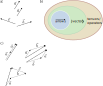
\includegraphics[scale=1.0]{arrowsAndVectors}
  \caption{Arrows provide a simple geometric example of vector quantities. The idea of vectors, however, is more powerful and extends beyond this simple representation as directed line segments.}
  \label{fig:arrowsAndVectors}
\end{figure}

Symbolically, we will denote vectors by placing an arrow over letters:
\[
\vec{a}\,,\vec{b}\,,\vec{c}\,,\ldots\,,\vec{\alpha}\,,\vec{\beta}\,.
\]
However, not all vectors behave like arrows. Futhermore, to introduce the basic notation of quantum theory as early as possible, we will switch to what is known as \emph{Dirac notation} for vectors.

\subsection{Dirac Notation}
Instead of placing an arrow on top of a letter, we enclose the letter between a pair of symbols as follows:
\[
\vec{a}\to\ket{a}\,.
\]
The advantages of this notation accumulate and become more apparent the longer we study quantum physics.

\subsection{Arrow Algebra}
Arrows are \emph{numberlike} -- they can be added and multiplied, and the rules for addition and multiplication resemble those of regular numbers. However, arrows allow a richer set of operations compared to numbers. For example, there are three different types of multiplication for any pair of arrows, depending on the type of the final result: 1) a number; 2) another arrow; 3) more complex geometric figures like a piece of a plane. We will mainly focus on the first type, called \emph{scalar product}, and the thrid one, called \emph{tensor product}.

\subsection{Bases}
Consider a pair of non-parallel arrows $\ket{a}$ and $\ket{b}$, arranged for convenience tail-to-tail. Their sum yields the third arrow $\ket{c}$:
\[
\ket{c} = \ket{a} + \ket{b} = 1\ket{a}+1\ket{b}\,.
\]
The numbers in front of $\ket{a}$ and $\ket{b}$ are called \emph{components} of the arrow $\ket{c}$ \emph{relative} to $\ket{a}$ and $\ket{b}$. By varying these numbers, while keeping the arrows $\ket{a}$ and $\ket{b}$ fixed, we can \emph{obtain any arrow in a plane}. In other words, any arrow $\ket{v}$ can be written as
\[
\ket{v} = v_a\ket{a}+v_b\ket{b}\,.
\]
Here, again, the pair of numbers $(v_a, v_b)$ represent components of $\ket{v}$ relative to $\ket{a}$ and $\ket{b}$. 

Non-parallel arrows $\ket{a}$ and $\ket{b}$ are \emph{independent}, in the sense that neither can be expressed in terms of the other. In contrast, the arrow $\ket{v} = v_a\ket{a}+v_b\ket{b}$ is not independent from $\ket{a}$ and $\ket{b}$. Thus, the set of arrows $\lbrace \ket{a}, \ket{b}, \ket{v} \rbrace$ is not independent. For arrows in a plane, the number of independent arrows can not be more than two -- matching the dimensionality of the plane.

The set of $n$ independent arrows is called \emph{basis} for the $n$-dimensional space in consideration. Any set of $m < n$ independent arrows will be \emph{incomplete} and insufficient to serve as a basis. In essense, basis is a set of "building blocks" for all possible arrows. The set of "building blocks" must be rich enough to build up anything else (\emph{complete set}), and it does not need any redundant elements (\emph{independent set}).

Basis in not unique, as we can easily show. Given basis $\ket{a}$ and $\ket{b}$, we can  rotate and scale each arrow separately, to obtain arrows $\ket{\alpha}$ and $\ket{\beta}$:
\[
\ket{a}\to\ket{\alpha}\,\textrm{ and }\,\ket{b}\to\ket{\beta}\,.
\]
As long as $\ket{\alpha}\nparallel\ket{\beta}$, they can be used as basis.
\begin{exercise}
	Consider $\ket{+} = \ket{a} + \ket{b}\,\textrm{ and }\,\ket{-}=\ket{a}-\ket{b}\,.$
	Prove that if $\ket{+}=\lambda\ket{-}$ then $\ket{b}=\mu\ket{a}$. Find $\mu$.
\end{exercise}
As the previous exercise shows, the arrows $\ket{+}$ and $\ket{-}$ are independent and can be used as basis.
\begin{exercise}
	Given $\ket{v}=\ket{a}+2\ket{b}$, express it in the $\lbrace \ket{+},\ket{-}\rbrace$ basis:
	\[
		\ket{v}=v_{+}\ket{+}+v_{-}\ket{-}\,.
	\]
	Find $v_{+}$ and $v_{-}$.
\end{exercise}

\subsection{Normalized Bases}
Vectors are sometimes defined as mathematical quantities with \emph{magnitude} and \emph{direction}. This implies that a meaningful notion of \emph{length} (magnitude) can be assinged to vectors. For arrows this is obvious, while for other types of vector-like quantities might be not so. 

The length of a vector is called its \emph{norm}. Vectors with unit length are called \emph{normalized}. Any vector can be "scaled" to have a unit length. Indeed, given a vector $\ket{a}$ with length $a$, we get a normalized vector as follows:
\[
\ket{u} = \frac{\ket{a}}{a}\,.
\]
When doing calculations, it is convenient to normalize all basis vectors. This results in \emph{normalized basis}.

\section{Scalar Product}
The first way to multiply two vectors that we will study is called \emph{scalar product}. In this operation two vectors are combined to yield a number (a.k.a \emph{scalar}):
\[
\ket{a}\cdot\ket{b} = x\,.
\]
Here we followed traditional \emph{infix notation} using "$\cdot$" as an analogue of "$*$" for numbers. Soon we will learn the usefulness of \emph{prefix notation} for scalar product and its relation to operators, but for now we will keep writing scalar product of vectors similar to numbers.

Guided by simplicity, we expect scalar product to satisfy two basic algebraic laws:
\[
\ket{a}\cdot\ket{b}  = \ket{b}\cdot\ket{a}\,\textrm{  -- commutativity}\,. 
\]
\[
(\ket{a}+\ket{b})\cdot\ket{c}=\ket{a}\cdot\ket{c}+\ket{b}\cdot\ket{c}\,\textrm{ -- distributivity }.
\]
Let's apply the last requirement to a vector $2\ket{a}$, representing it as $\ket{a}+\ket{a}$:
\[
(2\ket{a})\cdot\ket{b}=(\ket{a}+\ket{a})\cdot\ket{b}=\ket{a}\cdot\ket{b}+\ket{a}\cdot\ket{b}=2(\ket{a}\cdot\ket{b})\,.
\]
Thus, we see that one more requirement is both natural and helpful:
\[
(x\ket{a})\cdot\ket{b}=x(\ket{a}\cdot\ket{b})\,.
\]
We can formulate this last result as a rule: "scalars can be pulled outside."

\subsection{Products of Basis Vectors}
Combining scalar product with the representation of vectors in a \emph{normalized} basis $\lbrace 
\ket{u_1}, \ket{u_2}\rbrace$ leads to important insights. Consider two vectors:
\[
\ket{a}=a_1\ket{u_1}+a_2\ket{u_2}\,\textrm{ and }\,\ket{b}=b_1\ket{u_1}+b_2\ket{u_2}\,.
\]
Scalar product $\ket{a}\cdot\ket{b}$ can be calculated step-by-step, first expanding $\ket{a}$:
\[
\ket{a}\cdot\ket{b} = a_1\ket{u_1}\cdot\ket{b}+a_2\ket{u_2}\cdot\ket{b}\,.
\]
Then, expanding $\ket{b}$, we obtain:
\[
\ket{a}\cdot\ket{b}=a_1b_1\ket{u_1}\cdot\ket{u_1}+a_1b_2\ket{u_1}\cdot\ket{u_2}+a_2b_1\ket{u_2}\cdot\ket{u_1}+a_2b_2\ket{u_2}\cdot\ket{u_2}\,.
\]
Using the commutativity $\ket{u_1}\cdot\ket{u_2}=\ket{u_2}\cdot\ket{u_1}$, we can slightly simplify the last expression:
\[
\ket{a}\cdot\ket{b}=a_1b_1\ket{u_1}\cdot\ket{u_1}+(a_1b_2+a_2b_1)\ket{u_1}\cdot\ket{u_2}+a_2b_2\ket{u_2}\cdot\ket{u_2}\,.
\]
If the scalar products of all basis vectors are known, we can calculate scalar product of any pair of vectors. We reduced the problem to defining the scalar product of a pair of unit-length vectors:
\[
\ket{u_1}\cdot\ket{u_1}\,,\ket{u_2}\cdot\ket{u_2}\,,\textrm{ and }\ket{u_1}\cdot\ket{u_2}\,.
\]

The only difference between two unit-length vectors $\ket{u_1}$ and $\ket{u_2}$ is their orientation. Since there is no preferred direction in the plane, we can only speak of the \emph{mutual orientation} of the pair of vectors. A convenient measure of the mutual orientation is the \emph{angle between} corresponding arrows. We are, therefore, led to the following candidate for the scalar product:
\[
\ket{u_1}\cdot\ket{u_2} = f_\theta\,,
\]
where $\theta$ is the angle between $\ket{u_1}$ and $\ket{u_2}$, measured counterclockwise from $\ket{u_1}$ to $\ket{u_2}$. At this point, the only thing we can say about the function $f$ is that it is  continuous and periodic in its argument $\theta$. Let's examine two simple candidates -- trigonometric functions $\cos\theta$ and $\sin\theta$.

\subsection{Scalar Product Meaning}
Once the scalar product of two unit vectors is defined, we can ask what intuitive interpretation can be given to a scalar product in general. To this end, let's take a pair of normalized vectors $\ket{u_1}$ and $\ket{u_2}$ and scale them to an arbitrary lengths:
\[
\ket{u_1}\,\to\,\ket{a}=a\ket{u_1}\,\textrm{ and }\,\ket{u_2}\,\to\,\ket{b}=b\ket{u_2}\,.
\]
Scalar product of $\ket{a}$ and $\ket{b}$ is then simply
\[
\ket{a}\cdot\ket{b} = abf_\theta\,.
\]
The factor $ab$ -- the product of two lengths -- suggests that the scalar product is related to area, as illustrated in Figure \ref{fig:scalarProductMeaning}. 
\begin{figure}[htbp]
	\centering
	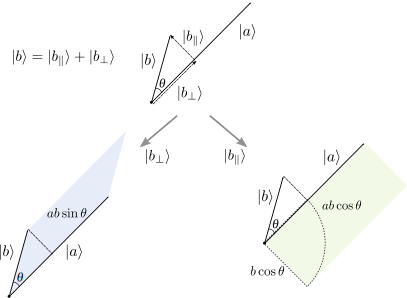
\includegraphics[scale=1.0]{scalarProductMeaning}
	\caption{Two way to interpret scalar product of two vectors.}
	\label{fig:scalarProductMeaning}
\end{figure}

If we note that the vector $\ket{b}$ can be written as the sum of two parts:
\[
\ket{b}=\ket{b_\parallel}+\ket{b_\perp}\,,
\]
 one parallel to the vector $\ket{a}$ and the other perpendicular to it, then two different interpretations can be given. First, if $f=\sin$, then the scalar product
\[
\ket{a}\cdot\ket{b} = ab\sin\theta
\]
would correspond to the area of a parallelogram built on two vectors $\ket{a}$ and $\ket{b}$ or the area of a rectangle built on two vectors $\ket{a}$ and $\ket{b_\perp}$. This approach is fruitful and it is used in a more advanced version of the product of two vectors, related to \emph{tensor product} as discussed later.

The second simple option corresponds to $f=\cos$ and the scalar product
\[
\ket{a}\cdot\ket{b} = ab\sin\theta\,.
\]
It is the area of the rectangle built on two vectors $\ket{a}$ and $\ket{b_\parallel}$. 

\begin{mybio}{Fidelity, Alignment, and Overlap}
	Scalar product of unit vectors can be viewed as the measure of their "alignment" or "overlap". This interpretation is useful in quantum theory, where vectors are used to represent states of quantum systems. 
\end{mybio}

\subsection{Orthonormal Bases}
The choice of basis vectors is dictated by their usefulness in a given problem. In many cases it is convenient to use basis vectors which have unit length and which are \emph{mutually orthogonal}:
\[
\ket{u_1}\cdot\ket{u_1}=1=\ket{u_2}\cdot\ket{u_2}\,\textrm{ and }\,\ket{u_1}\cdot\ket{u_2}=0\,.
\]
In this case scalar product of any two vectors 
\[
\ket{a}=a_1\ket{u_1}+a_2\ket{u_2}\,\textrm{ and }\,\ket{b}=b_1\ket{u_1}+b_2\ket{u_2}\,.
\]
takes on a very simple form:
\[
\ket{a}\cdot\ket{b}=a_1b_1+a_2b_2\,.
\]
Although we arrived at this result analysing only two-dimensional case, it is easily generalized to any number of dimensions. For an $n$-dimensional case we would have the following expression for the scalar product
\[
\ket{a}\cdot\ket{b}=\int a_ib_i\,,\quad  i=\overline{1,n}\,.
\]


\section{Operators}\label{sec:operators}
Operators are functions of a particular kind. A "usual" function, like $\cos$, \emph{transforms} a number into another number, while an operator $\op{T}$ transforms a vector into another vector:
\[
\op{T}\,\ket{a} = \ket{b}\,.
\]
It is better to consider examples.
\begin{mybio}{Example Operators}\\
	It is easy to come up with examples of operators:
	
	\begin{itemize}
		\item\phantom{x}
		
		\item Unit operator (or \emph{identity} operator), such that
		\[
		\op{I}\,\ket{a}=\ket{a}\,.
		\]
		
		\item ``Zeroing'' operator that maps every vector into a zero
		vector:
		\[
		\op{0}\, \ket{a} = \ket{0}\,.
		\]
		
		\item ``Flipping'' operator that changes a vector into its opposite:
		vector:
		\[
		\op{F}\, \ket{a} = -\ket{a}\,.
		\]
		
		\item ``Orthogonal'' operator that makes any vector perpendicular to its original direction. In other words, it rotates the original vector by $90$ degrees counter-clockwise, leaving the length the same:
		\[
		\op{J}\, \ket{a} = \ket{b}\,,\textrm{ such that }\, b=a\,\textrm{ and }\,\ket{a}\cdot\ket{b}=0\,.
		\]
		Here $a$ and $b$ are the lengths of the vectors.
		
		\item ``Normalizing'' operator that turns an arbitrary vector into a normalized vector with the same direction:
		\[
		\op{N}\, \ket{a} = \ket{a}/a\,.
		\]
		
		\item Rotation operators that perform a rotation of a vector by a specified angle $\theta$:
		\[
		\op{R}_\theta\, \ket{a} = \ket{b}\,,\textrm{ such that }\, a=b\,,\textrm{ and } \,\ket{a}\cdot\ket{b}=a^2\cos\theta\,.
		\]
		Special cases of these operators are $\op{F}=\op{R}_\pi$, $\op{J}=\op{R}_{\pi/2}$ and $\op{I}=\op{R}_0$.
		
		\item Scaling operators that change the length of a given vector by a specified factor:
		\[
		\op{S}_x\, \ket{a} = x\ket{a}\,.
		\]
		Special cases of these operators are $\op{F}=\op{S}_{-1}$, $\op{I}=\op{S}_1$, and $\op{0}=\op{S}_0$.
		
	\end{itemize}
\end{mybio}

\subsection{Operator Algebra}
Since operators are functions, we can manipulate them like functions. In particular, we can use them as objects in their own right, which can be added or composed. Indeed, if we can add vectors, we can give useful meaning to the sum of operators:
\[
\op{T} = \op{I} + \op{J} + \op{S}_2\,.
\]
To fully describe an operator, we must find how it acts \emph{on any} vector. In this example we get
\[
\op{T}\,\ket{a} = \op{I}\,\ket{a} + \op{J}\,\ket{a} + \op{S}_2\,\ket{a}=\ket{a}+\ket{b}+2\ket{a}=3\ket{a}+\ket{b}\,,
\]
where the vector $\ket{b}$ is orthogonal to $\ket{a}$, while having the same length.

Operators can be multiplied by "usual" numbers, and they can be composed.


\subsection{Linear Operators}
Among the simplest non-trivial operators are \emph{linear operators}. As mentioned earlier, linear functions satisfy two conditions:
\[
\op{T}\,(\ket{a}+\ket{b}) = \op{T}\,\ket{a}+\op{T}\,\ket{b}\,,
\]
and
\[
\op{T}\,(x\ket{a}) = x\op{T}\,\ket{a}\,.
\]
Thus, operator action distributes over a sum, and numbers can be pulled outside.

To define a linear operator, we need only to describe how it affects basis vectors. Indeed, if an arbitrary vector $\ket{a}$ is represented in some basis, we can write
\[
\op{T}\,\ket{a} = \op{T}\,(a_1\ket{u_1}+a_2\ket{u_2}) = \op{T}\,(a_1\ket{u_1})+\op{T}\,(a_2\ket{u_2})\,,
\]
and then pull numbers outside to obtain:
\[
\op{T}\,\ket{a} = a_1\op{T}\,\ket{u_1}+a_2\op{T}\ket{u_2}\,.
\]
We only need to know $\ket{t_1}=\op{T}\,\ket{u_1}$ and $\ket{t_2}=\op{T}\ket{u_2}$, so that 
\[
\op{T}\,\ket{a}=a_1\ket{t_1}+a_2\ket{t_2}\,,\quad \op{T}\,\ket{b}=b_1\ket{t_1}+b_2\ket{t_2}\,,\textrm{ and so on}.
\]
Now both $\ket{t_1}$ and $\ket{t_2}$ are vectors and can be represented in the same basis as $\ket{a}$:
\[
\ket{t_1}=T_{11}\ket{u_1}+T_{12}\ket{u_2}\,,
\]
and
\[
\ket{t_2}=T_{21}\ket{u_1}+T_{22}\ket{u_2}\,.
\]
The four numbers $T_{11},\,T_{12},\,T_{21}$, and $T_{22}$ are called \emph{components of an operator} in a given basis. It is crucial to remember that these components are specific to a basis. If we decide to change to a different basis, components of all vectors and operators will change.

\begin{mybio}{Matrix}
	Components of a linear operator in a given basis are often written as square table, called \emph{matrix}:
	\[
	\op{T} =
	\begin{pmatrix}
		T_{11} & T_{12}\\
		T_{21} & T_{22}
	\end{pmatrix}\,.
	\]
	We emphasize again: If we change to a different basis, components of the operators will change, and the matrix will look different. Sometimes matrices are convenient for computations, but they are rarely used in this book.
\end{mybio}

\begin{example}
	Consider an operator that transforms the state $\ket{0}$ into a linear combination $\ket{+}=(\ket{0}+\ket{1})/\sqrt{2})$ and the state $\ket{1}$ into a linear combination $\ket{-}=(\ket{0}-\ket{1})/\sqrt{2})$.
	
	It is called \emph{Hadamard} operator and has the following matrix representation.
\end{example}

\begin{mybio}{Numbers On Steroids}
	Operators can be used to solve problems that do not have solutions in terms of real numbers. For example:
	\[
	\op{A}+\op{B} = 6\op{I}\,\textrm{ and }\, \op{A}\op{B}=36\op{I}\,.
	\]
	To simplify this problem we can first rescale the operators, introducing
	\[
	\op{a} = \op{A} / 6\,\textrm{ and }\, \op{b} = \op{B}/6\,.
	\]
	\[
	\op{a}+\op{b} = \op{I}\,\textrm{ and }\, \op{a}\op{b}=\op{I}\,.
	\]
	
\end{mybio}

\subsection{Super-operators*}
An idea of a function is quite general, it implies mapping one value to another, or calculting result given a certain input. Given a number, a function can yield another number, or given a vector a function can produce another vector. In the latter case we call the function an \emph{operator}.  

In the mathematical toolset of both classical and quantum physics there are functions of \emph{higher order} in the sense that they can act on functions or operators. For example,  a \emph{super-operator} is a mapping from any operator $\op{T}$ into another operator. Although it sounds abstract, it is not a complicated idea. Indeed, all we need is a rule that finds some operator $\op{B}$ given an operator $\op{A}$. One non-trivial rule can be stated as follows: Given an operator $\op{A}$, apply it twice:
\[
\op{A}\quad\overset{\mathcal{F}}{\longrightarrow}\quad\op{B}=\op{A}\circ\op{A}\,.
\]
Since the composition of two operators is again an operator, this is a satisfactory definition.


\section{Functionals}
Another important type of function is called \emph{functional}. A functional maps a function into a number. Let's consider several examples.

\begin{flushleft}
	{\it Total Mass}
\end{flushleft}
Suppose an astrophysicist is trying to model a spherically symmetric star and calculates \emph{density} of the star as the function of distance from its center: $r\rightarrow\rho_r$. The total mass of the star can then be evaluated as the sum of masses of all spherical shells with thickness $\delta r$:
\[
M = \int \delta V\rho_r=\int 4\pi r^2\delta r\rho_r\,.
\]
For a given function $\rho_r$ this summation will result in a number -- star's total mass. Such mapping $\rho_r\rightarrow M$ is an example of a functional.

\begin{flushleft}
	{\it Total Fuel}
\end{flushleft}
Consider a car moving on a straight highway between two points $A$ and $B$. The amount of fuel the engine consumes at a given moment depends on the speed of the car at that moment and can be described by the function $\mu_v$. Suppose the position of the car as the function of time $x_t$ is known and are looking for the total fuel consumed during the travel. This can be done in three steps. 

First, we find the speed of the car as the function of time by applying the operator $\partial_t$ to $x_t$: $v_t=\partial_{t}x$. Second, we find the fuel consuption rate $\mu$  as the function of time by plugging $v_t$ into $\mu_v$: $f_t = \mu(v_t)$. Finally, we can find the total amount of consumed fuel as the sum
\[
F = \int f_t\delta t\,.
\]
Combining all three steps into a single mathematical expression will result in a more cumbersome formula:
\[
F = \int \delta t\mu(\partial_t x)\,.
\]
This formula encodes a recipe for mapping any function $x_t$ into a number $F$ -- an example of a functional.

\begin{flushleft}
	{\it Total Action}
\end{flushleft}
A body in a "free fall" is moving with constant acceleration due to the force of gravity. Its speed increases as the body approaches the ground. If the body starts at rest at height $H$, its position along the vertical $y$ axis depends on time as $y_t=H-gt^2/2$ and the velocity changes according to the equation $v=-gt$.

The potenital energy $E_p=mgy$ of the body decreases, while its kinetic energy $E_k=mv^2/2$ grows. The total mechanical energy $E=E_p+E_k$ remains fixed according to the law of energy conservation. Thus, the potential energy of the body is transformed into the kinetic energy.

Another physical quantity is often important -- the \emph{imbalance} of kinetic energy over the potential energy:
\[
L = E_k - E_p\,.
\]
It does not remain constant, and for the case of a free fall we can easily find its time dependence:
\[
L_t = mg^2t^2 - mgH\,.
\]
Given $L_t$, we can calculate a fundamental physical quantity -- total \emph{action} of the process:
\[
A = \int\delta t L_t\,.
\]
The summation extends to the moment $t=T$ when the body reaches the ground ($y=0$). This happens at $T=\sqrt{2H/g}$.

Performing the summation requires evaluation of two familiar sums:
\[
\int t^2\delta t =\frac{T^3}{3}\quad\textrm{ and }\quad \int \delta t=T\,.
\]
Substituting the values of $T$ and simplifying, the expression for the total action takes the form
\[
A = mgT(\frac{gT^2}{3}-H)=-\frac{mH}{3}\sqrt{2gH}=-\frac{mv_{m}H}{3}\,.
\]
Here we used $v_m=gT=\sqrt{2Hg}$ -- the maximal speed of the body at the end of the free fall process. Finally, denoting the maximum momentum of the body as $p_m=mv_m$, we obtain $A=-p_m H/3$. Note that the action can be expressed as the product of momentum and distance.

\emph{Action} is a physical quantit of fundamental importance. It plays a prominent role in both classical mechanics (the principle of \emph{stationary action}) and in quantum physics (the principle of \emph{action quantization}). Both principles will be explored in details later in the book.

\begin{exercise}
	Calculate the total action of a free fall process for an electron falling from the height 0.1 meter.
\end{exercise}


\begin{flushleft}
	{\it Assorted Examples}
\end{flushleft}
Examples of functionals given above involve evaluation of sums in order to find  \emph{total quantities} of various kinds:
\[
Q = \int \delta x f_x\,.
\]
The total quantity $Q$ depends on the behavior of the input function $f_x$ over an extended range of $x$ values. Simpler forms of functionals can also be used. For example:
\[
\mathcal{M}\, f = f_0
\]
returns the value of the input function $f_x$ at zero. This functional, despite its trivial look, is very useful and widely used in physics and mathematics. Its rigorous mathematical form is called \emph{Dirac delta function}\,.
\begin{mybio}{Dirac Delta Function}
	The idea of delta function is simple: it describes the density of mass (or charge, probability, and so on) for a point-like particle. Formally, such density can be written as $\delta_x$.
	
	Since the total mass (charge, probability) is finite, the summation of the density over the region where the particle might be must be a fixed number:
	\[
	m = \int \delta x \delta_x\,.
	\]
\end{mybio}

Another example of a simple functional is the maximum of a function:
\[
\mathcal{X}\,f = \textrm{max}\,f_x\,.
\]
Finally, one can map any function $f_x$ into a number like so:
\[
\mathcal{R}\,f = \frac{f_1}{1!} + \frac{f_{1/2}}{2!} + \frac{f_{1/3}}{3!}+\ldots+\frac{f_{1/n}}{n!}+\ldots\,.
\]
For $f=\sin$ we obtain $\mathcal{R}\,\sin\approx 1.1479$.
\begin{exercise}
	For the functionals $\mathcal{M}$, $\mathcal{X}$, and $\mathcal{R}$ check whether they are \emph{linear}.
\end{exercise}

\section{Spaces}
In mathematics and physics the concept of \emph{space} becomes more abstract, in comparison with the intuitive view of space as a "container for things." Space in mathematical sense is more akin to how people understand space in expressions like "space of ideas", "space of solutions", "color space", "design space", "parameter space", and so on.

First of all, space is a set of mathematical objects of similar nature. For example, all numbers, or all arrows considered as one single entity, can be viewed as space. Second, unlike a simple set, space has some \emph{structure}, some \emph{relations} between its elements. For example, there might some sense of direction, or distance, or simply the notion of continuity. Advanced spaces, used in mathematical physics, have quite a complex structure, with distances, angles, algebraic operations, and even with operations required for calculus.

We will be mainly using \emph{vector spaces}, understood as rich collections of all vectors, endowed with addition and multiplication operations, as defined earlier.

\section{Duality}
Many mathematical concepts have very natural "companions", related in the spirit of mirror images or "yin-yang." In this kind of relationship both "companions" are on equal footing, neither concept is preferred, neither is basic while the other is derived. This situation is called \emph{duality}.

Scalar product of vectors leads to two interesting and useful dualities. The first duality deals with vectors and results in \emph{dual vectors}, while the second duality deals with operators and gives the notion of \emph{adjoint operators}.

\subsection{Dual Vectors}
To arrive at dual vectors we can start with scalar product, written using a \emph{prefix notation}:
\[
\lbrack\cdot\rbrack\,\ket{a}\,\ket{b} = x\,.
\]
Here we introduced a binary operator (function of two vector arguments) that maps a pair of vectors into a number.

The next step is to consider the operator $\lbrack\cdot\rbrack$ \emph{partially applied} to the first argument only:
\[
\lbrack\cdot\rbrack\,\ket{a}\tus\,.
\]
Although here we denoted "an empy slot" with a grey circle $\tus$, it is unnecessary and can be dropped. Furthermore, we will use Dirac notation for the mathematical object that results from the partial application of scalar product, writing it as follows:
\[
\bra{a} = \lbrack\cdot\rbrack\,\ket{a}\,.
\]
Such an object can be written for \emph{every} vector:
\[
\bra{b} = \lbrack\cdot\rbrack\,\ket{b}\,,\quad
\bra{c} = \lbrack\cdot\rbrack\,\ket{c}\,,\quad\textrm{ and so on.}
\]

A beautiful thing about this whole construction is that it gives us \emph{new kinds of vectors}. Also, it teaches us a lesson that vectors can be viewed as functions, revealing a connection between the two concepts.

It is easy to demonstrate that $\bra{a}$ is a linear function. Recall that a function with two arguments, when partially applied, becomes a function of a single argument. Therefore, since $\lbrack\cdot\rbrack$ is the function of two vector arguments, $\bra{a}$ must be the function of just one vector argument. Moreover, since $\lbrack\cdot\rbrack$ is linear in both arguments, $\bra{a}$ must be linear in its single argument. More explicitely:
\[
\bra{a}\,(\ket{b}+\ket{c})=\bra{a}\ket{b}+\bra{a}\ket{c}\,.
\]
To check this equality, we first replace $\bra{a}$ with its definition, then switch to the infix notation, and use the distributivity of scalar product.
\begin{exercise}
	Prove the equalities:
	\[
	\bra{a}\,(\ket{b}+\ket{c})=\bra{a}\ket{b}+\bra{a}\ket{c}\,,
	\]
	and
	\[
	\bra{a}\,(x\ket{b})=x\bra{a}\ket{b}\,.
	\]
\end{exercise}
\begin{mybio}{Bra, Ket, and Braket}
	In Dirac notation the application of $\bra{a}$ to $\ket{b}$ is written in a less noisy way:
	\[
	\braket{a}{b}\,.
	\]
	The whole expression is called \emph{bracket}, whereas $\bra{a}$ is called \emph{bra vector}, and $\ket{b}$ is called \emph{ket vector}.
\end{mybio}

Now how can we show that the collection of objects $\bra{a}$, $\bra{b}$, $\bra{c}$ and so on forms a vector space? To be a vector an object must behave like one, demonstrating all properties that fully define vector. We will examine whether bra-vectors can be added, and whether they can be expanded in some basis.

Can $\bra{a}$ and $\bra{b}$ be added? Of course they can, because they are functions over "addable things" (over vectors), and the meaning of $\bra{v}=\bra{a}+\bra{b}$ is simple:
\[
\braket{v}{c}=\braket{a}{c}+\braket{b}{c}\,.
\]
For similar reasons, any $\bra{a}$ can be multiplied by "usual" numbers, so that the expressions like
\[
\bra{w} = x\bra{a}+y\bra{b}
\]
have a straightforward interpretation.

Since there is exists a basis in the ket-vector space, there is one in the bra-space. Indeed, suppose we have $\ket{a}=a_1\ket{u_1}+a_2\ket{u_2}$ and we use the linearity of the scalar product in its first argument:
\[
\bra{a} = \lbrack\cdot\rbrack\,(a_1\ket{u_1}+a_2\ket{u_2})=a_1(\lbrack\cdot\rbrack\,\ket{u_1})+
a_2(\lbrack\cdot\rbrack\,\ket{u_2})\,.
\]
Since
\[
\lbrack\cdot\rbrack\,\ket{u_1} = \bra{u_1}\,,\quad\textrm{ and }\quad\lbrack\cdot\rbrack\,\ket{u_2} = \bra{u_2}\,,
\]
we conclude that any bra-vector can be expanded in terms of some other bra-vectors, just like ket-vectors are expanded in some basis:
\[
\bra{a} = a_1\bra{u_1}+a_2\bra{u_2}\,.
\]
In summary, if we need a bra-basis, we can use ket-basis and partially apply the scalar product operator to each ket-basis vector. 

One last step is needed to rigirously prove that both ket-vectors and bra-vectors are indeed vectors: we must investigate how their components change when we change bases. The only challenge this task presents is its tediousness (REF TO MY BOOK).

From now on we will recognize that to every ket-vector $\ket{a}$ there corresponds a \emph{dual} bra-vector $\bra{a}$. We must remember that this duality is generated by the operation of scalar product. Once a vector space has scalar product defined, we get a dual vector space "for free." Such dual vector space turns out extremely useful in quantum theory, as we will soon see.

\subsection{Dual Operators}
\begin{figure}[htbp]
	\centering
	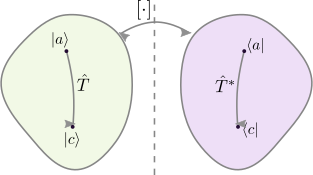
\includegraphics[scale=1.0]{adjointOperator}
	\caption{Duality generated by the scalar product applies both the vector spaces and operators acting on them.}
	\label{fig:adjointOperator}
\end{figure}
We have shown that each vector $\ket{a}$ has dual $\bra{a}$, and the whole space of ket-vectors has a dual counterpart, as shown in Figure \ref{fig:adjointOperator}. Given an operator $\op{T}$ acting on ket-space, we can define an operator $\op{T}^*$ acting on bra-space. The action of  $\op{T}^*$ on an arbitrary bra-vector $\bra{a}$ is defined as follows: we first transform bra-vector $\bra{a}$ into its dual ket-vector $\ket{a}$ and find $\op{T}\ket{a}=\ket{c}$, and finally find its dual $\bra{c}$, by partially applying scalar product:
\[
\bra{c}=(\op{T}\ket{a})\cdot\tus\,.
\]
This procedure maps any $\bra{a}$ into some $\bra{c}$, as required. Let's examine how this bra-vector $\bra{c}$ acts on an arbitrary ket-vector $\ket{b}$:
\[
\braket{c}{b}=(\op{T}\ket{a})\cdot\ket{b}\,.
\]
\begin{mybio}{Postfix Notation}
	The action of an operator $\op{T}$ on a ket-vector $\ket{a}$ is nearly always written using \emph{prefix notation}:
	\[
	\op{T}\ket{a}=\ket{c}\,.
	\]
	To emphasize the distinction between dual vector spaces, the application of the dual operator $\op{T}^*$ on the dual vector $\bra{a}$ follows \emph{postfix notation}:
	\[
	\bra{a}\op{T}^*=\bra{c}\,.
	\]
	The use of prefix-postfix notations highlights the "mirror-like" relationship between the dual objects:
	\[
	\bra{a}\op{T}^*\,\,\Bigg\vert\,\,\op{T}\ket{a}
	\]
\end{mybio}

\begin{mybio}{Conjugation}
	Switching between dual objects -- vectors or operators -- is an important and often used operation in quantum theory. This operation is called \emph{conjugation} and is often denoted by an asterisk:
	\[
	\ket{a}\quad\overset{*}{\longrightarrow}\quad\bra{a}\,,
	\]
	\[
	\op{T}\quad\overset{*}{\longrightarrow}\quad\op{T}^*\,,
	\]
	\[
	\op{T}\ket{a}\quad\overset{*}{\longrightarrow}\quad\bra{a}\op{T}^*\,.
	\]
	Another, more traditional, way to express these relations is as follows:
	\[
	\bra{a} = (\ket{a})^*\,,\quad \textrm{ and }\quad \bra{a}\op{T}^*=(\op{T}\ket{a})^*\,.
	\]
\end{mybio}

\subsection{Adjoint Operators}
The notion of an \emph{adjoint} operator is very important in quantum theory. Before we define it, we'll explore the context in which adjoint operator is used.

To begin, recall that a linear operator transforms an input vector into an output vector. For some operators such transformation is always \emph{reversible}: There exist another operator that can "cancel" the action of the first, as illustrated in Figure \ref{fig:dualOperators}(a), where the operator $\op{U}$ acts as the \emph{inverse} of the operator $\op{T}$:
\[
\op{U}\circ\op{T}=\op{I}\,.
\]
The inverse of an operator, if there exists one, is denoted using the negative power: $\op{U}=\op{T}^{-1}$. Not every operator has an inverse, with $\op{0}$ ("zeroing" operator) and $\op{N}$ (normalizing operator) being simple examples.

Scalar product leads to more sophisticated relations between operators. One such relation, shown in Figure \ref{fig:dualOperators}(b), amounts to one operator being "inverse relative to the second input" of the scalar product. In simpler terms: \emph{Acting on both inputs changes nothing}. This can be expressed in the following equation:
\[
\ket{a}\cdot\ket{b}=(\op{T}\ket{a})\cdot(\op{U}\ket{b})\,.
\]
If this equality holds true for \emph{any} pair of vectors $\ket{a}$ and $\ket{b}$, then we will call the operator $\op{T}$ \emph{scalar-inverse} of the operator $\op{U}$. All rotation operators $\op{R}_\theta$ are scalar-inverse of themselves:
\[
\ket{a}\cdot\ket{b}=(\op{R}_\theta\ket{a})\cdot(\op{R}_\theta\ket{b})\,.
\]
Indeed, rotating both vectors by the same angle, does not change their mutual orientation and does not affect their lengths, keeping the product $ab\cos\theta$ constant.
\begin{exercise}
	Find the scalar-inverse of the scaling operator $\op{S}_x$.
\end{exercise}
\begin{figure}[htbp]
	\centering
	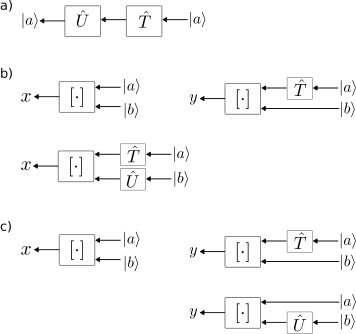
\includegraphics[scale=1.0]{dualOperators}
	\caption{Some operators have "relatives" which have certain interesting properties.}
	\label{fig:dualOperators}
\end{figure}

One more useful relation is generated by the scalar product. As illustrated in Figure \ref{fig:dualOperators}(c), this relation means that one operator, say $\op{T}$, achieves the same affect as the other operator (e.g. $\op{U}$), while acting on the second input of the binary scalar product operator $\lbrack\cdot\rbrack$. Symbollically we can write:
\[
\ket{a}\cdot(\op{U}\ket{b})=(\op{T}\ket{a})\cdot\ket{b}\,.
\]
If this is true for all possible vectors, then we will call the operator $\op{T}$ \emph{scalar-equivalent} to the operator $\op{U}$.  A conventional name for the scalar-equivalent operator is \emph{adjoint}. From the definition given above it is clear that both the original operator $\op{U}$ and its adjoint $\op{T}$ act on the same ket-vector space. The adjoint of the operator $\op{U}$ is often denoted using "\emph{dagger}"-notation:
\[
\op{T}=\op{U}^\dagger\,.
\]
\begin{mydef}{Adjoint Operator}
	An adjoint of the operator $\op{U}$ acting on ket-space, is another operator, denoted as $\op{U}^\dagger$, acting on the same ket-space, and satisfying the following requirement:
	\[
		\ket{a}\cdot(\op{U}\ket{b})=(\op{U}^\dagger\ket{a})\cdot\ket{b}
	\]
	\emph{for all} pairs of ket-vectors.
\end{mydef}

All scaling operators $\op{S}_x$ are scalar-equivalent to themselves:
\[
\ket{a}\cdot(\op{S}_x\ket{b})=(\op{S}_x\ket{a})\cdot\ket{b}\,.
\]
Indeed, scaling the first vector by some factor $x$ has the same effect on the product $ab\cos\theta$ as scaling the second vector by the same factor.
\begin{exercise}
	Find the scalar-equivalent of the rotation operator $\op{R}_\theta$.
\end{exercise}

Interestingly, finding the adjoint of a given operator is simpler than finding its inverse. This is most easily done using components:
\[
U_{ij} = \ket{u_i}\cdot(\op{U}\ket{u_j})=(\op{U}^\dagger\ket{u_i})\cdot\ket{u_j}\,,
\]
now we can use the commutativity of the scalar product
\[
U_{ij} = \ket{u_j}\cdot(\op{U}^\dagger\ket{u_i})=U^\dagger_{ji}\,.
\]
Thus, the components of the adjoint $U^\dagger_{ji}$ are obtained from the components of the operator $U_{ij}$ by "swapping" indices. For example:
\[
U^\dagger_{11} = U_{11}\,,U^\dagger_{22} = U_{22}\,,\quad\textrm{ and so on, while}
\]
\[
U^\dagger_{12} = U_{21}\,,U^\dagger_{23} = U_{32}\,,\quad\textrm{ and so on.}
\]
\begin{mybio}{Transposition}
	The swapping of components $T_{ij}\to T_{ji}$ is called \emph{transposition}, and the resultant operator whose components are $T_{ji}$ is called \emph{transposed} relative to the original operator $\op{T}$.
\end{mybio}

The concepts of conjugation and adjoint operator, discussed above, have interesting and powerful representations in terms of \emph{tensor product} -- the topic of the next section.


\section{Tensor Product}
A pair of vectors can be combined in a variety of ways, yielding results of different kinds, see Figure \ref{fig:vectorOperations}. 
Two familiar operations of vector addition and scalar product are close analogs of numeric addition and multiplication, respectively. Addition "glues" two vectors into the third vector, scalar product "fuses" two vectors into a number. There exists one more method of "bundling" vectors which results not in a number or yet another vector, but in a more advanced mathematical objects called \emph{tensor}. Tensors are closely related to operators and we will focus on this aspect of tensor product. 
\begin{figure}[htbp]
	\centering
	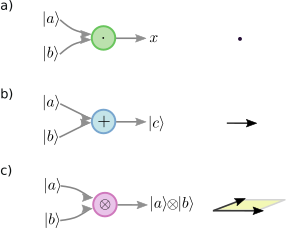
\includegraphics[scale=1.0]{vectorOperations}
	\caption{Three basic operation with vectors: a) Scalar product; b) vector sum; c) tensor product.}
	\label{fig:vectorOperations}
\end{figure}

We start with a pair of ket-vectors $\ket{a}$ and $\ket{b}$ and try "bundling" them in a way that resembles multiplication. Denoting this new operation $\otimes$, we want to have 
\[
\ket{a}\otimes\left(\ket{b}+\ket{c}\right)=\ket{a}\otimes\ket{b}+\ket{a}\otimes\ket{c}\,,
\]
and
\[
(x\ket{a})\otimes(y\ket{b})=xy\ket{a}\otimes\ket{b}\,.
\]
The last requirement indicates that this new type of product has the nature of an area, since it is proportional to the product of the lengths of two vectors. Thus, it can't be another vector, but must be a construction of different kind that we will call \emph{tensor}, and the product $\ket{a}\otimes\ket{b}$ -- a \emph{tensor product}. 

Using the arrow model of vectors, we can consider as a possible candidate a "blade" -- a piece of plane swept by "sliding" the vector $\ket{a}$ along the vector $\ket{b}$, as illustrated in Figure \ref{fig:vectorOperations}(c). This geometric object has "magnitude" or size, defined by the area of the blade, and it has direction or orientation. This approach is used in geometric algebra, where the \emph{outer product} is defined along these lines.

The geometric representation of product $\ket{a}\otimes\ket{b}$ might be appealing, but not at all required. Furthermore, it might even be unhelpful when we would like to generalize the operation to the product of other vector types:
\[
\ket{a}\otimes\bra{b}\,,\quad \bra{a}\otimes\ket{b}\,,\quad\textrm{ or }\quad\bra{a}\otimes\bra{a}\,.
\]
In other words, we should not constrain ourselves by reliance on a geometric intuition. How then do we interpret these various products? Well, one simple \emph{operational} criterion helps: A mathematical object is defined by \emph{what it does} and \emph{how it is used}. Let's study the two most important cases of tensor products.

\subsection{Ket-Ket}
The first tensor product is made of two ket-vectors:
\[
\op{P} = \ket{a}\otimes\ket{b}\,.
\]
In quantum theory, where ket-vectors "store" the information of all possible measurement (\emph{state} of a quantum system), the product is used to describe a \emph{joint system}, in which two distinct parts, say $A$ and $B$, can be identified and measured by different measuring devices.
\begin{figure}[htbp]
	\centering
	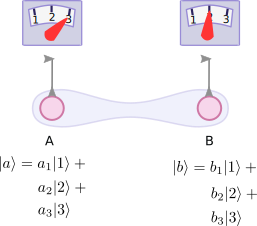
\includegraphics[scale=1.0]{ketketExample}
	\caption{Joint measurement of two systems.}
	\label{fig:ketketExample}
\end{figure}


Let's study an example, shown in Figure \ref{fig:ketketExample}. Imagine that we measure the value of some discrete quantity (quantized energy of an atom, for instance) using identical devices in different locations, corresponding to the systems $A$ and $B$. Suppose that in each trial the value of energy is measured to be either 1, or 2, or 3 \emph{randomly}. Then, after many trials of measuring the energy of the system $A$, we may summarize the statistics as follows:
\[
\ket{a}=a_1\ket{1}+a_2\ket{2}+a_3\ket{3}\,,
\]
where $a_i=N_i/N$ is the \emph{probability} to obtain the result $i$, expressed as the ratio of the number of times $N_i$ the value $i$ appeared in a series of $N$ measurements. Similarly, after many trials of measuring the energy of the system $B$, we may summarize the statistics as an expression:
\[
\ket{b}=b_1\ket{1}+b_2\ket{2}+b_3\ket{3}\,,
\]
with the similar meaning of the coefficients $b_i$.

Now we can write the summary of observation of two systems joined together:
\[
\op{P} = \ket{a}\otimes\ket{b}=a_1b_1 \ket{1}\otimes\ket{1}+a_1b_2 \ket{1}\otimes\ket{2}+\ldots a_3b_3 \ket{3}\otimes\ket{3}\,.
\]
From the probability theory it is known (see SECTION X) that the numbers $p_{ij}=a_ib_j$ give the probability to measure the value $\ket{i}$ in the experiment on the system $A$, while getting the value $\ket{j}$ in the measurement performed on $B$.

It might seem like unnecessary complication to use the tensor product expressions like
\[
\op{P} = \int p_{ij}\ket{i}\otimes\ket{j}
\]
instead of keeping separate vectors $\ket{a}$ and $\ket{b}$. But if we try to use individual vectors $\ket{a}$ and $\ket{b}$ when the results of joint measurements have the following statistics:
\[
\op{P}_0 = \frac{1}{2} \ket{1}\otimes\ket{1}+\frac{1}{2} \ket{2}\otimes\ket{2}\,,
\]
we discover that no $\ket{a}$ and $\ket{b}$ satisfy the requirement $\op{P}_0=\ket{a}\otimes\ket{b}$.
\begin{exercise}
	Prove that the assumption 
	\[
	\op{P}_0=\ket{a}\otimes\ket{b}
	\]
	leads to contraditions and, therefore, can not be true.	
\end{exercise}
The information encoded in the tensor product $\op{P}_0$ is an example of \emph{strongly correlated} behavior. In this example, it says that whenever system $A$ is found (randomly!) with the energy $1$, the same energy is measured on the system $B$; similarly for the energy $2$. Effects like these are of great interest in quantum theory, and the operation of tensor product is indispensable for describing such phenomena.


\subsection{Ket-Bra}
The second type of tensor product involves one ket-vector and one bra-vector, "bundled" into a new object which behaves like an \emph{operator}, unlike braket used in scalar product. Given vectors $\ket{a}$ and $\bra{b}$, we can form a tensor product
\[
\op{P}=\ket{a}\otimes\bra{b}\,.
\] 
\begin{mybio}{Economical Notation}
	Instead of writing $\ket{a}\otimes\ket{b}$ we will often write $\ket{a}\ket{b}$. Instead of $\ket{a}\otimes\bra{b}$ we will often write $\ket{a}\bra{b}$.
\end{mybio}
What does $\op{P}$ do? It can be used as an operator, acting on ket-vectors as follows:
\[
\op{P}\ket{c}=\ket{a}\otimes\bra{b}\ket{c}=\ket{a}\braket{b}{c}=x\ket{a}\,,
\]
where $x=\braket{b}{c}$ is a number. The operator $\ket{a}\otimes\bra{b}$ transforms any input vector into a vector parallel to $\ket{a}$. In other words, it \emph{projects} all vectors onto the direction specified by $\ket{a}$. Operators of this kind are sometimes called \emph{projectors}, but we will reserve this name for the operators of special form $\ket{a}\otimes\bra{a}$.
\begin{exercise}
	Suppose $\ket{a}\perp \ket{b}$ and $\op{P}=\ket{a}\otimes\bra{b}$. Find the result of $\op{P}\ket{a}$ .
\end{exercise}
\begin{mydef}{Projector}
	A tensor product $\ket{a}\otimes\bra{a}$ is called \emph{projector}. It projects all vectors onto the direction specified by the vectors $\ket{a}$, while only scaling $\ket{a}$:
	\[
	\ket{a}\otimes\bra{a}\ket{a}=a^2\ket{a}\,.
	\]
\end{mydef}

In quantum theory ket-vectors represent the state of a quantum system -- the information about all possible measurement results. Projectors like $\ket{a}\otimes\bra{b}$ describe the change of state $\ket{b}\to\ket{a}$, or \emph{transition} between states. 

Another application of tensor products in quantum theory is representation of \emph{operators} in a choses basis. To see this, recall that every linear operator is fully specified once we know how it transforms basis vectors:
\[
\op{T}\ket{a}=\op{T}(a_1\ket{u_1}+a_2\ket{u_2})=a_1(\op{T}\ket{u_1})+a_2(\op{T}\ket{u_2})\,.
\]
If $\op{T}\ket{u_1}=\ket{t_1}$, then we can express it using tensor product $\op{P}_1=\ket{t_1}\otimes\bra{u_1}$. The transormation of $\ket{u_2}$ can be written similarly: $\op{P}_2=\ket{t_2}\otimes\bra{u_2}$. Since $\op{P}_1$ and $\op{P}_2$ are both operators, they can be multiplied by numbers and added to obtain another operator. The action of $\op{T}$ then becomes expressed as
\[
\op{T}\ket{a}=a_1\op{P}_1\ket{u_1}+a_2\op{P}_2\ket{u_2}=\op{P}_1(a_1\ket{u_1})+\op{P}_2(a_2\ket{u_2})\,.
\] 
Now since 
\[
\op{P}_1(a_1\ket{u_1})=\op{P}_1(a_1\ket{u_1}+a_2\ket{u_2})=\op{P}_1 \ket{a}\,,
\]
and
\[
\op{P}_2(a_2\ket{u_2})=\op{P}_2(a_1\ket{u_1}+a_2\ket{u_2})=\op{P}_2 \ket{a}\,,
\]
because of the orthogonality of the basis. For example:
\[
	\op{P}_1(a_2\ket{u_2})=a_2\ket{t_1}\otimes\bra{u_1}\ket{u_2}=0\,.
\]

The action of the operator $\op{T}$ becomes
\[
\op{T}\ket{a}=\op{P}_1\ket{a}+\op{P}_2\ket{a}=\left(\op{P}_1+\op{P}_2\right)\ket{a}\,.
\]
Now we can drop the input ket-vector, writing the operator in terms of the ket-bra tensor products:
\[
\op{T}=\ket{t_1}\otimes\bra{u_1}+\ket{t_2}\otimes\bra{u_2}\,.
\]
We can leave the expression as is or convert it into tensor product of only basis vectors. Recalling that 
\[
\ket{t_1}=T_{11}\ket{u_1}+T_{12}\ket{u_2}\,,\quad\textrm{ and }\quad \ket{t_2}=T_{21}\ket{u_1}+T_{22}\ket{u_2}\,,
\]
and using the linearity of the tensor product, we arrive at the following exression:
\[
\op{T}=T_{11}\ket{u_1}\bra{u_1}+T_{12}\ket{u_1}\bra{u_2}+
T_{21}\ket{u_2}\bra{u_1}+T_{22}\ket{u_2}\bra{u_2}\,.
\]
Here we used the \emph{economical notation} for tensor product. It can be further compactified and generalized to any number of dimensions:
\[
\op{T}=\int T_{ij}\ket{u_i}\bra{u_j}\,,\quad i,j=\overline{1,n}\,.
\]
\subsection{Useful Ket-Bras}
A unit operator $\op{I}$ plays an important role in many calculations. It can be represented as 
\[
\op{I}=\int\ketbra{u_i}{u_i}\,,\quad i=\overline{1,n}\,.
\]
It is easy to check this for $n=2$ explicitely:
\[
(\ketbra{u_1}{u_1}+\ketbra{u_1}{u_1})\ket{a}=\ket{u_1}\braket{u_1}{a}+\ket{u_2}\braket{u_2}{a}\,.
\]
The right-hand side is clearly the expansion of the ket-vector $\ket{a}$ in the basis $\ket{u_i}$:
\[
\ket{u_1}\braket{u_1}{a}+\ket{u_2}\braket{u_2}{a}=a_1\ket{u_1}+a_2\ket{u_2}=\ket{a}\,.
\]
\begin{mybio}{Completeness}
	The expression
	\[
	\op{I}=\int\ketbra{u_i}{u_i}\,,\quad i=\overline{1,n}\,
	\]
	is called the \emph{completeness} statement of the set of basis vectors. It says that the set of orthonormal vectors is \emph{not missing} any vector necessary to construct all other vectors in the space. Indeed, if we omit even a single term $\ketbra{u_k}{u_k}$ in the sum $\int\ketbra{u_i}{u_i}$ then the term $a_k\ket{u_k}$ will be missing in the expansion
	\[
	\left(\int\ketbra{u_i}{u_i}\right)\ket{a}=a_1\ket{u_1}+\ldots+a_{k-1}\ket{u_{k-1}}+a_{k+1}\ket{u_{k+1}}+\ldots a_n\ket{u_n}\,.
	\]
\end{mybio}

The operator $\op{J}$ that rotates vectors in a plane by 90 degrees counter-clockwise takes the basis ket-vector $\ket{u_1}$ into $\ket{u_2}$ and $\ket{u_2}$ into $(-\ket{u_1})$. Using tensor products $\op{J}$ can be written as follows:
\[
\op{J}=\ketbra{u_2}{u_1}-\ketbra{u_1}{u_2}\,.
\]


\subsection{Tensor Product of Operators}


\begin{exercise}
	Write Hadamard operator in terms of the tensor product of vectors $\ket{0}$, $\ket{1}$, $\ket{+}$ and $\ket{-}$.
	
	\[
	\op{H} = \ketbra{+}{0}+\ketbra{-}{1}\,.
	\]
\end{exercise}

\section{Functions As Vectors}
Perhaps surprisingly, but certain classes of functions, which are very useful in physics, have all characteristic of vectors. 

\section{Application: Circular Motion}
Let us examine how the concepts and tools discussed above can be applied to a simple case of circular motion.  

Consider a  particle moving in a circle with the radius $R$, as shown in Figure X. If we choose the center of the circle as the reference point, we can specify the position of the particle using an arrow $\ket{r}$. During motion the direction of this arrow is constantly changing, but its length $R$ remains the same.  

After a short time interval $\delta t$, the position of the particle changes by $\delta\ket{r}$:
\[
\ket{r_t}\quad\rightarrow\quad \ket{r_{t+\delta t}} = \ket{r_t}+\delta\ket{r}\,.
\]

The length of the path covered by the particle during the time interval $\delta t$ can be approximated by the length of the arc  $\delta L=R\delta\theta=v\delta t$. The arrow $\delta\ket{r}$ can be written as $\delta L\ket{u}$ where $\ket{u}$ is the vector of unit length pointing in the direction of motion. This unit vector can be constructed from $\ket{r}$ by scaling it down by $R$ and then rotating counter-clockwise with the operator $\op{J}$: 
\[
\delta\ket{r}=R\delta\theta\op{J}\left(\frac{\ket{r}}{R}\right)\,.
\]
Since $\op{J}$ is a linear operator, the $R$ cancels and we can write
\[
\frac{\delta\ket{r}}{\delta t}=\frac{\delta\theta}{\delta t}\op{J}\ket{r}\qquad\Longrightarrow\qquad
\partial_t\ket{r}=\omega\op{J}\ket{r}\,,
\]
where we introduced the angular speed $\omega=\partial_t\theta$. Finally, by applying the $\op{J}$ operator to both sides of the last equation, we can cast it into the "Schrodinger" form:
\[
\op{J}\partial_t\ket{r}=-\omega\ket{r}\,.
\]  




\section*{Chapter Highlights}
{\setstretch{1.5}\chhc
  \it
\begin{itemize}
\item Arrows in a plane provide a simple model for vectors.
\item Arrows can be manipulated in ways analogous to numbers: Two arrows
  be added, an arrow can be ``scaled'' (stretched or compressed). Arrows form
  an algebra.
\item Basis is an extremely important concept. Basis is a set of
  objects (arrows) that can be used to ``build'' all other similar
  objects (arrows). At the same time, basis can not be used to build
  itself -- basis arrows are independent.
\end{itemize}
}

%

%----------------------------------------------------------------------------------------
%	PART
%----------------------------------------------------------------------------------------
%\part{Part B}

\chapterimage{pics/chapterImageOperators.pdf}
\graphicspath{{../04ClassicalPhysics/pics/}}

\chapter{Classical Physics}\label{ch:ClassicalPhysics}
\begin{quoting}
	I think we may ultimately reach the stage when
	it is possible to set up quantum theory without any reference to classical theory,
	just as we already have reached the stage where we can set up the Einstein
	gravitational theory without any reference to the Newtonian theory. But
	from the point of view of teaching students, I think one would always
	have to proceed by stages -- not expect too much from them, teach them
	first the elementary theories and gradually develop their minds; and
	that will always involve working from the classical theory
	first.
	
	P. A. M. Dirac, Lectures on Quantum Field Theory, Belfer Graduate
	School of Science, Yeshiva University, New York, 1966, p.43.
\end{quoting}

\lettrine[lines=2]{\color{darkocre}T}{he} concept of
\emph{operators}\index{Operator} extends the idea of functions. An unary numeric
function $f$ takes some numeric value $x$ as an input  and produces
another numeric value $y$:
\[
f\,x=y\quad \textrm{ or } \quad x\overset{f}{\longrightarrow} y\,.
\]
In mathematical jargon, $f$ \emph{maps} $x$ into $y$.

\begin{myprereq}{Prerequisite Knowledge}
	To fully understand the material of this chapter, readers should be comfortable with the following concepts:
	
	\begin{itemize}
		\item \phantom{phantom}
		\vspace{-0.5cm}
		\item State
		\item Dynamical equations
	\end{itemize}	
\end{myprereq}


\begin{figure}[htbp]
  \centering
  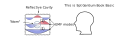
\includegraphics[scale=1.0]{defaultFigureTemplate}
  \caption{Operators extend the idea of functions. (a) An unary
    function $f$ can be applied to a number $x$ to produce
    another number $y$. (b) An unary operator $\op{F}$ can be applied to a vector
    $\vec{a}$ to yield another vector $\vec{b}$.}
  \label{fig:arrowsOperatorGeneral}
\end{figure}

\section{System}\label{sec:System}
A part of nature that can be clearly isolated and studied is called a \emph{physical system}. An electron, an atom, a molecule, a crystal, a pendulum, a comet, a star – these are examples of physical systems of various degrees of complexity.

Often a physical system is a body or several bodies interacting with each other or with some external bodies. Figure \ref{fig:systemExamples} provides several examples of \emph{mechanical systems}. Let’s examine them in more detail.
\begin{figure}[htbp]
	\centering
	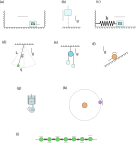
\includegraphics[scale=1.0]{systemExamples}
	\caption{Examples of mechanical systems. See text for explanation..}
	\label{fig:systemExamples}
\end{figure}
\renewcommand{\labelenumi}{(\alph{enumi})}
\begin{enumerate}
	\item \emph{Free falling body}: An elastic body falls down vertically under the
	force of gravity, bounces back, goes up and then down to repeat the
	bounce again and again. Also, a projectile launched at an angle.
	\item \emph{String pendulum}: A compact body is attached to a string
	of fixed length. It is allowed to swing back and forth without
	experiencing air friction.
	\item \emph{Atwood machine}: Two bodies with slightly unequal masses
	are connected with a non-stretchable string going over a
	frictionless pulley.
	\item \emph{Inclined plane}: A solid cylinder rolling down an
	inclinded plane.
	\item \emph{Piston}: A system of three bodies (cylindrical
	crankshaft, rod, and piston) connected in a way that locks rotation
	of a cylinder and the vertical motion of the piston.
	\item \emph{Spring oscillator}: A body, attached to a spring, is
	allowed to slide left and right across a frictionless surface.
	\item \emph{Linear chain of oscillators}: A set of pairwise
	interconnected identical bodies; the allowed motion happens along
	the horizontal axis.
	\item \emph{Sun and planet}: A planet circling around the sun.
	
\end{enumerate}
We will study oscillator and circular motion in great detail.

\subsection{Configuration}
In mechanics, \emph{configuration} means a formal way to describe the
arrangement of a system at a given time.

The behavior of a system in time can be described by specifying its
\emph{configuration} as the function of time. In relatively simple
systems, configuration may consist of a set of coordinates that uniquely
determine the arrangement of bodies in the system. For example, the
configuration of a pendulum can be given by a single coordinate --- the
length of the arc $q$. Of course, as the pendulum swings, both
Cartesian coordinates $x$ and $y$ are changing, but not independently,
due to the relation
\begin{equation*}
	x^2 + y^2 = L^2\, .
\end{equation*}
Given $x$, we can find $y > 0$ as $y = +\sqrt{L^2 - x^2}$, thus
reducing the number of required coordinates.

Consider another example, shown in the Figure
(\ref{fig:coupledSystem})(a): a system of
two bodies, connected with each other using ideal springs with
stiffness $k$, and each body is connected to a rigid wall.
\begin{figure}[htbp]
	\centering
	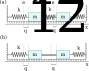
\includegraphics[scale=1.0]{coupledSystem}
	\caption{(a); (b).}
	\label{fig:coupledSystem}
\end{figure}

When the system is in equilibrium, the bodies occupy positions on the
horizotal axis denoted as $e_1$ and $e_2$. During motion, the position
of the first body changes by
\begin{equation*}
	q_1(t) = x_1(t) - e_1\, ,
\end{equation*}
and similarly for the second body: $q_2 = x_2 - e_2$. It is important
to realize, that although the two bodies are connected with a spring,
they can still move with different velocities, and have different
displacements $q_1 \ne q_2$. Indeed, we can set the system in motion
by moving each body independently and then releasing them. Contrast
this with the situation, shown in the Figure
(\ref{fig:coupledSystem})(b), where the bodies are connected with a
rigid rod, fusing two masses into essentially a single body. In this
case only a single displacement $q$ is required to specify the
configuration of the system.

\subsection{Qoordinates}
The coordinates specifying the configuration of a system do not
have to be Cartesian. In the example of a pendulum, the configuration
can be conveniently given by the length of the arc $q=L\theta$, see
Figure (\ref{fig:systemExamples})(b).

Consider another example, shown in the Figure
(\ref{fig:systemExamples})(h): Two bodies interact
gravitationally. In this problem, it turns out, the equations
describing the motion of the system are simpler if, instead of the
usual positions $x_1$ and $x_2$ we use the relative distance
\begin{equation*}
	q_1 = x_2 - x_1
\end{equation*}
and the position of the center of mass
\begin{equation*}
	q_2 = (m_1x_1 + m_2x_2)/(m_1 + m_2),
\end{equation*}
where $m_1$ and $m_2$ are the masses of the bodies.

We thus come to the idea of \emph{generalized coordinates} --
arbitrary coordinates completely specifying the configuration of a
system. Generalized coordinates can be based on positions, angles, or
some combinations of those.

\subsection{Degrees of Freedom}
\emph{Degree of freedom} is a separate independent motion of a
mechanical system. Each independent motion corresponds to the change
in time
of a separate generalized coordinate. The number of degrees of freedom
is the number of
generalized coordinates required to completely specify the
configuration of a mechanical system at different moments of time.

Take, for example, a pendulum, shown in the Figure
(\ref{fig:degreeOfFreedomPendulum}). In general Cartesian coordinates,
all three coordinates $x$, $y$, and $z$ will be changing in
time. However, only a single generalized coordinate $q(t)$ --- the
length of the arc -- is required to fully describe the configuration,
and thus the motion, of this mechanical system. The number of degrees
of freedom, in this example, equals 1.

\begin{figure}[htbp]
	\centering
	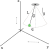
\includegraphics[scale=1.0]{degreeOfFreedomPendulum}
	\caption{A pendulum has one degree of freedom, despite the fact
		that all three Cartesian coordinates can be changing during its motion.}
	\label{fig:degreeOfFreedomPendulum}
\end{figure}




\section{Oscillator}\label{sec:Oscillator}
The model of an oscillator is extremely important. It appears in
various guises in almost all physical theories. Let's study it in details.

\begin{figure}[htbp]
	\centering
	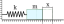
\includegraphics[scale=0.9]{Oscillator}
	\caption{A mechanical model of an oscillator: A body attached to an
		ideal spring.}
	\label{fig:Oscillator}
\end{figure}


Consider a body with the mass $m$ is attached to a spring with the stiffness
$k$. The body is allowed to move across a frictionless
surface.  The force required to strech a spring by the amount $x$
is given by the Hooke's law
\[
F=kx.
\]
This is the force applied \emph{to the spring}. The force created
\emph{by the spring, and applied to the attached body}, is of equal
magnitude but points in the opposite direction.

When the body is displaced from its equilibrium position,
by stretching or compressing the spring, and then released, it will
undergo periodic motion. During this motion, the position, velocity,
kinetic energy of the mody, and the potential energy of the spring
will be constantly changing.

To remind, the kinetic energy of a body is

\[
E_{k}=\frac{mv^{2}}{2}, \textrm{ or } K = \frac{p^2}{2m}\,.
\]
The potential energy of a spring, stretched or compressed by the
amount $x$ is given by

\[
E_{p}=\frac{kx^{2}}{2}, \textrm{ or } \Pi = \frac{kq^2}{2}\,.
\]


\section{State}\label{sec:State}
\emph{State} of a system is the \emph{minimal} collection of observables which is, in
certain sense, \emph{complete} and \emph{self-sufficient}. State is 
"all there is to know" about a system. If the state of a system is known at one
moment of time $t_0$, then we should be able to determine the state
at any later moment of time $t$. In classical mechanics the pair of
observables $(x, p)$ defines the state of a mechanical system.

\emph{State} is the minimal set of quantities describing mechanical
system and sufficient to predict
their future values from their initial values. State is an important
concept not only mechanics, but in other areas of physics.
Let's elaborate, using the oscillator as an example.

Suppose that at the moment of time $t_{0}$the position of the oscillator
is $x_{0}$ and its velocity is $v_{0}$. To find their values at
some later time $t>t_{0}$, we can go iteratevly in small steps, calculating
how much the position and the velocity change after each successive
tiny interval of time $\delta t$. The first iteration results in
the updated value of position
\begin{equation}
	x_{1}=x_{0}+v_{0}\delta t.
\end{equation}

The second, and every other, iteration looks very similar:
\begin{equation}
	x_{2}=x_{1}+v\delta t\,.
\end{equation}

Now it is important to realize that we can no longer use the same initial
velocity $v_{0}$in the second iteration, because the velocity itself
changes. Thus, we must update the value of the velocity as well. This
is done by using acceleration:
\begin{equation}
	v_{1}=v_{0}+a_{0}\delta t.
\end{equation}

Once this is done, we can find the second iteration of the position:
$x_{2}=x_{1}+v_{1}\delta t$. To keep this scheme going, we must be
able to update the value of the acceleration, because it is also changing.
It appears then, we need some quantity that allows to find the next
step:
\begin{equation}
	a_{1}=a_{0}+b_{0}\delta t,
\end{equation}
but, fortunately, \emph{this is not required!} At this point we can use the laws of motion.
For example, the Newton's second law allows us to find the acceleration,
if we know the force acting on the object:
\begin{equation}
	a=\frac{F}{m}.
\end{equation}

All physical forces, it appears, depend on positions (distances) and,
sometimes, velocities of bodies. The force of the spring $F=-kx$, for example,
depends only on the coordinate $x$. The force of gravitational interaction $F=GMm/r^2$
and the Coulomb force between two charges $F=kQq/r^2$ both depend on the distance
$r$ between the bodies. The force acting on an electron moving through
a magnetic field $F=qvB$ depends on the electron's velocity (and the field's strength $B$). 
No known forces depend on acceleration. This fact leads to an important conclusion:
It is enough to know position and velocity of an object at time $t_{0}$,
in order to find their values at any later moment of time $t>t_{0}$.
Obviously, position and velocity at any previous moment of time can
be found in the similar way.

Thus, we do not need to advance the acceleration by calculating its
small change $\delta a=b\delta t$, we can simply calculate it from
the law of motion:
\begin{equation}
	a_{n}=\frac{F(x_{n},v_{n})}{m}\,.
\end{equation}

This formula says that the acceleration at the iteration step number
$n$ is found from the values of the position $x_{n}$ and the velocity
$v_{n}$ at the same step. Given the velocity, we can advance the
postion, and given the acceleration, we can advance the velocity.
Then we recalculate the new value for the acceleration and repeat,
until we reach the final time $t$.

The preceding discussion demonstrates that in Newtonian mechanics
\emph{the state of a mechanical system} is given by a pair of quantities
-- $(x,v)$. There are alternatives to the Newtonian mechanics, and,
correspondingly, there are alternatives to the mechanical state. The
first such alternative is Hamiltonian dynamics.

\subsection{State Evolution: Newtonian Approach}
We will now apply the ideas and formulas of Newtonian mechanics to an
oscillator. We will calculate the motion of the oscillator in time
using a simple method of \emph{state evolution}. Specifically, we will
setup two simple equations -- one for position and one for velocity.

The equation for position is trivial and amounts to the definition:
\[
\frac{\delta x}{\delta t} = v\,.
\]
The equation for velocity follows from the second law of Newtonian
dynamics:
\[
\frac{\delta v}{\delta t} = \frac{F}{m} = -\frac{kx}{m}\,.
\]
Here we used the expression for the spring force $F=-kx$ acting
\emph{on the body} from the side of the spring.

Suppose we know the \emph{initial state} of the oscillator
$(x_0, v_0)$ at time $t_0=0$. When the clock makes a single tick after
a tiny time interval $\delta t$ the body will move to a new position
\[
x_1 = x_0 + v_0\delta t
\]
and the velocity will change due to the action of the spring:
\[
v_1 = v_0 -\frac{kx_0}{m}\,.
\]
Thus, after a single tick of the clock the state of the oscillator
will evolve from $(x_0, v_0)$ to $(x_1, v_1)$. At this point we can
keep repeat the steps to calculate the state after any number of
ticks, up to the desired time $t=N\delta t$.

We can now formalize the recipe for evolution of the state and write a
mathematical function
\[
(x_{new}, v_{new}) = f\, (x_{old}, v_{old}) = (x_{old}+v_{old}\delta
t, v_{old} - kx_{old}/m)\,.
\]
\begin{figure}[htbp]
	\centering
	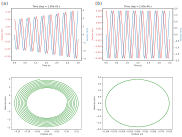
\includegraphics[scale=0.9]{newtonianStateEvolution}
	\caption{First row: Position (red curve, left axis) and velocity (blue
		curve, right axis) as functions of time. Second row: Velocity vs position.
		(a) Calculations with time step of 1 millisecond. (b) Calculations
		with time step of 1 microsecond.}
	\label{fig:newtonianStateEvolution}
\end{figure}

Using this simple approach, we can calculate the state $(x, v)$ of the
oscillator for any moment in the future or past. Figure
\ref{fig:newtonianStateEvolution} shows two example results. The first
result, in the column (a), demonstrates that we must be careful with
the step size $\delta t$ of the time. If it is not sufficiently small,
the inherent error of the method accumulates quickly, resulting in
wrong behavior, such as the gradual increase of velocity and
oscillation amplitude. The column (b) of Figure
\ref{fig:newtonianStateEvolution} demonstrates the expected behavior
of the oscillator -- periodic change of position with constant amplitude.

\section{Dynamics}\label{sec:Dynamics}
An action of an operator $F$ on arrows can be represented symbolically
as an equation.

\section{Hamiltonian}\label{sec:Hamiltonian}
An action of an operator $F$ on arrows can be represented symbolically
as an equation.

\section{Lagrangian}\label{sec:Lagrangian}
An action of an operator $F$ on arrows can be represented symbolically
as an equation.

\section{Field}\label{sec:Field}
An action of an operator $F$ on arrows can be represented symbolically
as an equation.

\section{Ideal Versus Real}\label{sec:IdealVsReal}
An action of an operator $F$ on arrows can be represented symbolically
as an equation.



\section*{Chapter Highlights}
{\setstretch{1.5}\chhc
  \it  
\begin{itemize}
\item Operators extends the idea of functions.
\item Numeric functions (e.g., $\sin\,x$) act on numbers and yield
  other numbers. Operators may act on vectors to yield other vectors
  or numbers.
\item Linear operators represent the simplest and yet powerful class
  of operators on vectors.
\item Linear operators can be represented graphically or symbolically.
\end{itemize}

}
%

\chapterimage{pics/chapterImageTensors.pdf}
\graphicspath{{../05QuantumPhysics/pics/}}

\chapter{Quantum Physics}\label{ch:QuantumPhysics}
\lettrine[lines=2]{\color{darkocre}T}{he} first type of operators -- and
corresponding tensors -- that we encountered has a simple type:
\[
\op{L}\,\vec{a} = \vec{b}\,.
\]
It is a linear unary function mapping vectors into vectors.


\begin{myprereq}{Prerequisite Knowledge}
To fully understand the material of this chapter, readers should be comfortable with the following concepts:

\begin{itemize}
	\item \phantom{phantom}
	\vspace{-0.5cm}
	\item State
	\item Dynamical equations
\end{itemize}	
\end{myprereq}

\section{Quantum System}\label{sec:QuantumSystem}
We are looking for a binary operator $\op{\sigma}$ that yields a number
based on two vectors:
\[
\ketbra{\sigma}{\sigma}\,\vec{a}\,\vec{b}=x\,.
\]

\section{Quantum State}\label{sec:QuantumState}
We are looking for a binary operator $\op{\sigma}$ that yields a number
based on two vectors:
\[
\ketbra{\sigma}{\sigma}\,\vec{a}\,\vec{b}=x\,.
\]
\subsection{States Overlap}
\[
\braket{\psi}{\phi}.
\]

\section{Quantum Dynamics}\label{sec:QuantumDynamics}
We are looking for a binary operator $\op{\sigma}$ that yields a number
based on two vectors:
\[
\ketbra{\sigma}{\sigma}\,\vec{a}\,\vec{b}=x\,.
\]

\section{Quantum Hamiltonian}\label{sec:QuantumHamiltonian}
We are looking for a binary operator $\op{\sigma}$ that yields a number
based on two vectors:
\[
\ketbra{\sigma}{\sigma}\,\vec{a}\,\vec{b}=x\,.
\]


\section{Quantum Bit}\label{sec:Qubit}
Any quantum system with two active states is called a \emph{qubit}. The state with lower energy is usually called \emph{ground state} and denoted as $\ket{g}$ or $\ket{0}$ (zero). The state with higher energy is usually called \emph{excited state} and denoted as $\ket{e}$ or $\ket{1}$ (one). The notation $\ket{0}\,,\ket{1}$ is used in the field of quantum information and computation.

If the energy of the ground and excited states are $E_g$ and $E_e$, respectively, then the Hamiltonian of a qubit can be written using projectors
\[
\op{H} = E_g\ketbra{g}{g}+E_e\ketbra{e}{e}\,.
\]
It requires an energy $\Delta E=E_e-E_g$ to excite the qubit from the lower energy state to the higher energy state. This energy may come from a quantum of electromagnetic field oscillating with frequency $\omega=\Delta E/\hbar$.

\subsection{Flipping Operator}
Transition between the states of a qubit can be described mathematically using operators that map one state into another. For example, an operator $\op{F}$ that \emph{flips} states must do the following:
\[
\op{F}\,\ket{0}=\ket{1}\,,\quad \op{F}\,\ket{1}=\ket{0}\,.
\]
Such operator can be easily built from the tensor products:
\[
\op{F} = \ketbra{1}{0}+\ketbra{0}{1}\,.
\]
Each term in this sum is useful in quantum theory. The first term is called \emph{raising operator} and is denoted as 
$ \op{\sigma}_\plus=\ketbra{1}{0}$. The second term is called \emph{lowering operator} and is denoted as $ \op{\sigma}_\minus=\ketbra{0}{1}$. Apparently, the raising operator excites the qubit from the ground state, while the lowering operator brings the qubit down from the excited state.

\begin{exercise}
	Calculate (a) $\op{\sigma}_\plus \op{\sigma}_\plus$; (b) $\op{\sigma}_\minus \op{\sigma}_\minus$; (c) $\op{\sigma}_\plus \op{\sigma}_\minus$; (d) $\op{\sigma}_\minus \op{\sigma}_\plus$.
\end{exercise}

\begin{exercise}
	Show that  $\op{\sigma}_\plus \op{\sigma}_\minus+\op{\sigma}_\minus \op{\sigma}_\plus=\op{I}$, where $\op{I}$ is the identity operator.
\end{exercise}

\begin{exercise}
	Show that the qubit Hamiltonian can be written in terms of the raising and lowering operators as follows:
	
	\[
	\op{H} = \hbar\omega\left(\op{\sigma}_\plus \op{\sigma}_\minus+\epsilon\op{I} \right)\,,
	\]
	where $\epsilon=E_g/\Delta E$.
\end{exercise}

\subsection{Number Operator}
The operator $\op{n}=\op{\sigma}_\plus \op{\sigma}_\minus$ is called \emph{number operator} for the following reason. First, note that $\op{\sigma}_\plus \op{\sigma}_\minus=\ketbra{1}{1}$ is the projector on the excited state of qubit.
 

\section{Quantum Oscillator}\label{sec:QuantumOscillator}
The \emph{principle of the quantization of action} can be applied to harmonic oscillator. The result is the quantization of energy levels. 

The energy of a harmonic oscillator can be expressed in terms of the maximum momentum $p_m$ or in terms of the maximum displacement $x_m$:
\[
H = \frac{p_m^2}{2m}\quad\textrm{ or }\quad H=\frac{kx_m^2}{2}\,.
\]
Multiplying these two equalities and recalling that $\omega^2=k/m$, we obtain
\[
H = \frac{\omega x_m p_m}{2}\,.
\]
The path which the state vector $\ket{\xi}=(x,p)$ follows in phase space is an ellipsis with the major semi-axes $x_m$ and $p_m$. The area of this ellipsis is $A=\pi x_m p_m$. Therefore, the connection between the energy of harmonic oscillator and the area is given by
\[
H=\frac{\omega}{2\pi}A\,.
\]
The area $A$ is a physical quantity with the units of action.

As shown in Figure \ref{fig:phaseSpaceQuantum}(a), areas in phase space have the smallest size limited by the elementary quantum of action $h$ -- known as Planck constant. The quantization of action and, consequently, the quantization of phase-space area, has two important implications for harmic oscillator.
\begin{figure}[htbp]
	\centering
	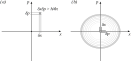
\includegraphics[scale=1.0]{phaseSpaceQuantum}
	\caption{Areas of phase-space regions have the units of action. Quantization of action implies quantization of phase-space area. (a) The smallest area in phase space is limited by the fundamental quantum of action $h$ -- Planck's constant. (b) Area of the ellipsis inside the path of harmonic oscillator is proportional to its energy. Quantization of area leads to the quantization of energy of harmonic oscillator.}
	\label{fig:phaseSpaceQuantum}
\end{figure}

First, every time an oscillator absorbs some energy $\Delta E$, the maximum deviation and the maximum momentum increase. The ellipsis in phase space increases its area. But since the area in phase space can't grow continiously--changes in discrete quanta $\delta A=h$--we must have discreete changes in energy. Second, the existence of the elementary quantum of action and the smallest are in phase space, require that the lowest energy state of harmonic oscillator is described not by a point in phase space, but by an elementary ellipsis such that $A_0=\delta x\delta p\propto h$. Putting these two ideas together, we conclude that the area of the ellipsis can be written as
\[
A_n = A_0 + nh\,.
\]
The energy of the oscillator then takes the form
\[
H=n\hbar\omega + E_0\,,
\]
where $\hbar=h/2\pi$ is called \emph{reduced Planck's constant}, and $E_0$ is the lowest energy of the harmonic oscillator. From the expression for $H$ follows that harmonic oscillator can be in a countable set of states, growing in energy from $E_0$ by a fixed step $\hbar\omega$. 

The energy of the lowest state can be written in terms of the step size $\hbar\omega$: $E_0=e_0\hbar\omega$, where $e_0$ is some number (it will be found later). Finally, we can write the energy of harmonic oscillator as follows:
\[
H=\hbar\omega(n + e_0)\,.
\]

\subsection{Hamiltonian Operator}
For any quantum system with descrete energy states $E_0, E_1, E_2,\ldots, E_n\ldots$ the Hamiltonian operator can be written in terms of projectors:
\[
\op{H}=\int E_k\ketbra{k}{k}\,,\quad k=0,1,2,\ldots,n\ldots 
\]
For harmonic oscillator $E_k=E_0+k\hbar\omega$ for $n>1$ and the Hamiltonian operator can be written as follows
\[
\op{H} = \int (E_0+k\hbar\omega)\ketbra{k}{k}\,.
\]
The number $k$ tells how many excitations quantum oscillator absorbed to reach the energy state $\ket{k}$.
Opening the parentheses and recalling that
\[
\int\ketbra{k}{k}=\op{I}\,,
\] 
we obtain 
\[
\op{H} = E_0\op{I}+\hbar\omega \int k\ketbra{k}{k}\,.
\]
This expression is very similar to the Hamiltonian of a qubit 
\[
\op{H}_{qb}=E_g\op{I}+\hbar\omega\op{n}
\]
where $\op{n}=\op{\sigma_\plus}\op{\sigma_\minus}$ is a number operator. The similarity is not accidental, as the operator $\op{n}=\int k\ketbra{k}{k}$ plays the role of the number operator. Indeed, it is easy to check by direction application that:
\[
\op{n}\,\ket{n}=n\ket{n}\,.
\]
In other words, the energy states $\ket{n}$ of harmonic oscillator, are the eigen-states of the number operator $\op{n}$ with the eigen-value $n$ corresponding to the number of excitation level.
\begin{exercise}
	Prove that $\op{n}\,\ket{n}=n\ket{n}$ by direction application of the operator $\op{n}=\int k\ketbra{k}{k}$.
\end{exercise}

The expression for the number operator $\op{n}$ can be obtained in a different way. First note that
\[
\op{H}\,\ket{n}=E_n\ket{n}\,,\quad\textrm{ where } E_n = E_0 + n\hbar\omega\,.
\]
From this follows
\[
(\op{H}-E_0\op{I})\,\ket{n}=n\hbar\omega\,\ket{n}\,,
\]
and, consequently, 
\[
\frac{(\op{H}-E_0\op{I})}{\hbar\omega}\,\ket{n}=n\,\ket{n}\,.
\]
The operator on the left hand side of this equation is the number operator $\op{n}$. It can be simplified once we recall that
\[
\op{H}=\int E_k\ketbra{k}{k}\quad\textrm{ and }\quad \op{I}=\int\ketbra{k}{k}\,.
\]
Using these relations, we first write
\[
\op{H}-E_0\op{I}=\int (E_k-E_0)\ketbra{k}{k}\,.
\]
Then, remembering that $E_k=E_0+k\hbar\omega$, we immediately arrive at
\[
\op{n}=\frac{(\op{H}-E_0\op{I})}{\hbar\omega}=\int k\ketbra{k}{k}\,.
\]
Thus, the operator of quantum harmonic oscillator can be written in the following form:
\[
\op{H}_{osc}=E_0\op{I}+\hbar\omega\op{n}\,.
\]
\subsection{Ladder Operators}
The number operator for qubit could be expressed as the product of two simple operators that raised or lowered qubit states:
\[
\op{n} = \op{\sigma}_\plus\op{\sigma}_\minus\,.
\]
The idea of raising and lowering states is also applicable to harmonic oscillator. Similar to qubit, we can write such operators as tensor products:
\[
\op{a}_\plus = \ketbra{n+1}{n}\textrm{ and }\quad\op{a}_\minus=\ketbra{n-1}{n}\,.
\]
Unfortunately, these operators will act properly only on the state $\ket{n}$.
\begin{exercise}
	Evaluate (a) $\op{a}_\plus \,\ket{n}$; (b) $\op{a}_\minus \,\ket{n}$; (c) $\op{a}_\plus \,\ket{n+m}$; (d) $\op{a}_\plus \,\ket{n+m}$.
\end{exercise}
It is easy to fix this problem by summing over all states:
\[
\op{a}_\plus=\int \ketbra{k+1}{k}\quad\textrm{ and }\quad \op{a}_\minus=\ketbra{0}{0}+\int \ketbra{m-1}{m}\,,\quad m > 0\,.
\]
The first term in the expression for $\op{a}_\minus$ ensures that the vacuum state remains unchanged: $\op{a}_\minus\,\ket{0}=\ket{0}$.
\begin{exercise}
	Evaluate (a) $\op{a}_\plus \,\ket{n}$; (b) $\op{a}_\minus \,\ket{n}$.
\end{exercise}
Let's check whether $\op{a}_\plus\op{a}_\minus$ yields the number operator $\op{n}=\int k\ketbra{k}{k}$. Even without explicitely evaluating the composition $\op{a}_\plus\op{a}_\minus$ we can see that it is unlikely to contain the required factor $k$.
\begin{exercise}
	Show that $\op{a}_\plus\op{a}_\minus=\ketbra{1}{0}-\ketbra{0}{0}+\op{I}$.
\end{exercise}

To find better operators for raising and lowering states of harmonic oscillator, we can taken a closer look at the qubit case. There we had $\op{\sigma}_\plus\,\ket{0}=1\ket{1}$ and $\op{\sigma}_\minus\,\ket{1}=1\ket{0}$\,. We explicitely added "1" in front of the final states, to highlight the following property of the $\op{\sigma}$-operators:
\[
\op{\sigma}_\plus\,\ket{k}=\sqrt{k+1}\ket{k+1}\quad\textrm{ and } \op{\sigma}_\minus\,\ket{k}=\sqrt{k}\ket{k-1}\,.
\]
Thus, we can "upgrade" the raising and lowering operators $\op{a}_\plus$ and $\op{a}_\minus$ to include the information about the state they act on. We want them to behave as follows:
\[
\op{a}_\plus\,\ket{k}=\sqrt{k+1}\ket{k}\quad\textrm{ and }\quad \op{a}_\minus\,\ket{m}=\sqrt{m}\ket{m-1}\,.
\]
\begin{exercise}
	Evaluate $\left(\op{a}_\plus\right)^p\,\ket{0}$.
\end{exercise}
\begin{exercise}
	(a) Show that the upgraded operators have the property 
	\[
	\op{a}_\plus\op{a}_\minus\,\ket{m}=m\ket{m}\quad m>0\,.
	\]	
	(b) Evalulate $\op{a}_\minus\op{a}_\plus\,\ket{m}$.
\end{exercise}
\begin{exercise}
	(a) Show that 
	\[
	\op{a}_\minus\op{a}_\plus-\op{a}_\plus\op{a}_\minus=\op{I}\,.
	\]	
\end{exercise}

Such raising and lowering operators (also called \emph{ladder operators}) are very useful when working with quantum harmonic oscillators. In terms of the ladder operators, the Hamiltonian of quantum oscillator is written as
\[
\op{H}_{osc} = \hbar\omega\op{n}+E_0\op{I}\,,
\]
where the number operator $\op{n}=\op{a}_\plus\op{a}_\minus$. 


\subsection{Conjugation}
The raising operator $\op{a}_\plus$ can be written in terms of the tensor products:
\[
\op{a}_\plus=\int_0 \sqrt{k+1}\ketbra{k+1}{k}\,.
\]
If we limit the lowering operator to states $\ket{m}$ with $m>0$, then it also allows a simple representation
\[
\op{a}_\minus=\int_1 \sqrt{m}\ketbra{m-1}{m}\,.
\]
By changing the summation variable $m-1=k$ (and, therefore, $m=k+1$), we can re-write the summation over $k=0,1,2\ldots$:
\[
\op{a}_\minus=\int_0 \sqrt{k+1}\ketbra{k}{k+1}\,.
\]
Now the expression for $\op{a}_\minus$ became similar to the expression for $\op{a}_\plus$, with the exception that the order of states in the tensor product is flipped:
\[
\ketbra{k+1}{k}\leftrightarrow \ketbra{k}{k+1}\,.
\]
This change of order of factors in a tensor product is called \emph{conjugation}. The operators $\op{a}_\minus$ and $\op{a}_\plus$ are therefore related to each other via the \emph{conjugation operation}. These operators are said to be \emph{conjugates} of each other. 

The relation of conjugation gives some insight into what the lowering operator $\op{a}_\minus$ does to the vacuum state:
\[
\op{a}_\minus\,\ket{0}=\int_0  \sqrt{k+1}\ket{k}\braket{k+1}{0}=0\int_0\sqrt{k+1}\ket{k}=0\ket{\infty}\,,
\]
where we introduced a vector 
\[
\ket{\infty}=\ket{0}+\sqrt{2}\ket{1}+\sqrt{3}\ket{2}+\ldots+\sqrt{n+1}\ket{n}+\ldots
\]
Obviously, $\ket{\infty}\ne\ket{0}$. The overall factor of zero negates any possible contributions of $\ket{\infty}$, making the product $0\ket{\infty}$ a special "zero vector" $\ket{z_0}$, with the natural property
\[
\ket{k}+\ket{z_0}=\ket{k}\,.
\]
The vector $\ket{z_0}$ does not correspond to any physical state, but represents a mathematical "zero vector". Since for all mathematical manipulations the vectors $0\ket{\infty}$ and $0\ket{0}$ are equivalent,
we can express the action of the lowering operator $\op{a}_\minus$ on the vacuum state as follows:
\[
\op{a}_\minus\,\ket{0}=0\ket{0}\,.
\]
Finally, the action of the number operator $\op{n}=\op{a}_\plus\op{a}_\minus$ on the vacuum state can be evaluated:
\[
\op{a}_\plus\op{a}_\minus\,\ket{0}=\op{a}_\plus(\op{a}_\minus\,\ket{0})=0(\op{a}_\plus\,\ket{0})=0\ket{1}=0\ket{0}\,,
\]
here we used the mathematical equivalence of states $0\ket{1}$ and $0\ket{0}$.

\begin{mybio}{Dagger Notation}
	The relation of conjugation between operators is denoted using a special notation. For example, if we denote the lowering operator $\op{a}_\minus$ simply as $\op{a}$, then its conjugate operator-- raising operator-- is denoted using a special "dagger" symbol as the superscript:
	\[
	\op{a}_\plus = \op{a}^\dagger\,.
	\]
	The use of dagger notation is standard in quantum theory. 
	
	Let's use the dagger notation to summarize the basis facts about the ladder operators, the number operator, and the Hamiltonian of quantum oscillator.
	First, raising and lowering properties:
	\[
	\op{a}\,\ket{n}=\sqrt{n}\ket{n-1}\,,\qquad\op{a}^\dagger\,\ket{n}=\sqrt{n+1}\ket{n+1}\,.
	\]
	Second, number operator and commutator:
	\[
	\op{a}^\dagger\,\op{a}\,\ket{n}=n\ket{n}\,,\qquad \op{a}\,\op{a}^\dagger-\op{a}^\dagger\,\op{a}=\op{I}\,.
	\]
	Finally, conjugation relation between the ladder operators:
	\[
	\op{a}\overset{\dagger}{\longrightarrow}\op{a}^\dagger\,.
	\]
\end{mybio}
\subsection*{Normal Order}
\begin{exercise}
	Ladder operators are used many important applications of quantum theory. Often one encounters expressions with several operators in no particular order, for example $\op{X}=\op{a}^\dagger\,\op{a}^2\,\op{a}^\dagger\,\op{a}$. For calculations it is necessary to rearrange these operators into a \emph{normal order} where all raising operators appear on the left, before the lowering operators.
	
	Use the commutation relation $\op{a}\,\op{a}^\dagger-\op{a}^\dagger\,\op{a}=\op{I}$ to put $\op{X}$ into a normal order.
\end{exercise}


\subsection{Canonical Commutation}
The Hamiltonian operator for quantum harmonic oscillator can be written in different ways. One way relies on energy eigen-values $E_k$:
\[
\op{H}=\int_0 E_k\ketbra{k}{k}\,.
\]
Another way utilizes raising and lowering operators:
\[
\op{H}=\hbar\omega \op{a}^\dagger\,\op{a}+E_0\op{I}\,.
\]
However, the starting point was the expression in terms of position and momentum. The question then becomes whether we can introduce \emph{position and momentum operators} such that for harmonic oscillator we get
\[
\op{H}=\frac{\op{p}^2}{2m}+\frac{m\omega^2\op{x}^2}{2}\,.
\]
We already saw in Exercise X the hint that some relationship must exist between the operators $\op{a}$, $\op{a}^\dagger$ and $\op{x}$, $\op{p}$. Such relationship must be linear in order to transform the expression for $\op{H}$ quadratic in terms of raising and lowering operator
\[
\op{H}=E_0\op{a}\,\op{a}^\dagger+(\hbar\omega-E_0)\op{a}^\dagger\,\op{a}=\square\,\op{a}\,\op{a}^\dagger+\square\, \op{a}^\dagger\,\op{a}
\]
into the expression quadratic in terms of position and momentum
\[
\op{H}=\square\, \op{p}^2+\square\, \op{x}^2\,.
\]
We are thus looking for a linear transformation
\[
\op{x} = A\,\op{a}+B\,\op{a}^\dagger\quad\textrm{ and }\quad \op{p}=C\,\op{a}+D\,\op{a}^\dagger
\]
which will lead to the Hamiltonian operator $\op{H}=E_0\op{a}\,\op{a}^\dagger+(\hbar\omega-E_0)\op{a}^\dagger\,\op{a}$.
\begin{exercise}
	Show that the Hamiltonian operator for harmonic oscillator in terms of the unknown coefficients $A, B, C$ and $D$ has the form:
	\begin{align*}
	\op{H}= & \left(\frac{C^2}{2m}+\frac{m\omega^2A^2}{2}\right)\op{a}^2+\left(\frac{D^2}{2m}+\frac{m\omega^2B^2}{2}\right)\op{a}^\dagger+\\
	+& \left(\frac{CD}{2m}+\frac{m\omega^2 AB}{2} \right)\op{a}\,\op{a}^\dagger+\left(\frac{CD}{2m}+\frac{m\omega^2 AB}{2} \right)\op{a}^\dagger\,\op{a}\,.
\end{align*}
\end{exercise}
\begin{exercise}
	Using the result of the previous exercise, show that it implies that $E_0=\hbar\omega/2$.
\end{exercise}
\begin{exercise}
	Using the results of the two previous exercises, show that the four unknown coefficients $A, B, C$ and $D$ satisfy the following equations:
	\[
	C^2=-(m\omega A)^2\,,
	\]
	\[
	D^2=-(m\omega B)^2\,,
	\]
	and
	\[
	CD+(m\omega)^2AB=m\hbar\omega\,.
	\]
\end{exercise}
\begin{exercise}
	Using the result of the previous exercise, show that $CD=(m\omega)^2AB$ (convince yourself that $CD$ can't be $CD=-(m\omega)^2AB$!). Then show that one possible solution is the set of coefficients:
	\[
	A=B=\sqrt{\frac{\hbar}{2m\omega}}\,,
	\]
	and
	\[
	C=-D=-\op{J}\sqrt{\frac{\hbar m\omega}{2}}\,.
	\]
\end{exercise}

With the steps outlined above, we obtain the following expressions for the operators of position and momentum:
\[
\op{x}=\sqrt{\frac{\hbar}{2m\omega}}\left(\op{a}^\dagger+\op{a}\right)
\]
and
\[
\op{p}=\op{J}\sqrt{\frac{\hbar m\omega}{2}}\left(\op{a}^\dagger-\op{a}\right)\,.
\]
Using these relations, it is now easy to find so called \emph{canonical commutation relation} for the basic physical operators of position and momentum. First, we find
\[
\op{x}\op{p}=\op{J}\frac{\hbar}{2}\left(\op{a}^\dagger\op{a}^\dagger-\op{a}\op{a}+\op{a}\op{a}^\dagger-\op{a}^\dagger\op{a}\right),
\]
then
\[
\op{p}\op{x}=\op{J}\frac{\hbar}{2}\left(\op{a}^\dagger\op{a}^\dagger-\op{a}\op{a}+\op{a}^\dagger\op{a}-\op{a}\op{a}^\dagger\right).
\]
Subtracting the latter equation from the former, we arrive at
\[
\lbrack \op{x},\op{p}\rbrack=\op{x}\op{p}-\op{p}\op{x}=\op{J}\hbar\lbrack \op{a},\op{a}^\dagger\rbrack=\op{J}\hbar\,.
\]

\section{Physical Realization of Qubits}
Recall that harmonic oscillator is any physical system with Hamiltonian
\[
H = \frac{p^2}{2m}+\frac{kx^2}{2}\,.
\] 
Many concrete physical systems can be described using this Hamiltonian and thus provide specific \emph{realizations} of 
the oscillator model. Similarly, many concrete physical systems realize the idea of a qubit.

\section{Interacting Qubits}\label{sec:InteractingQubits}
We are looking for a binary operator $\op{\sigma}$ that yields a number
based on two vectors:
\[
\ketbra{\sigma}{\sigma}\,\vec{a}\,\vec{b}=x\,.
\]
\subsection{Computational Basis}
\[
\ket{\Upsilon}_1 = \ket{0}\ket{0},\,\ket{\Upsilon}_2 = \ket{0}\ket{1},\,
\ket{\Upsilon}_3 = \ket{1}\ket{0},\,\ket{\Upsilon}_4 = \ket{1}\ket{1}\,.
\]
Q: Are there other states, which are also basis and product? Smth like
\[
\ket{\Xi}=\ket{+}\ket{+}\,.
\]

\subsection{Bell States}
\[
\ket{\Phi}^{+}\,,\quad\ket{\Phi}^{-}\,,\quad
\ket{\Psi}^{+}\,,\quad\ket{\Psi}^{-}\,.
\]


\subsection{GHZ State}\label{sec:GHZState}
We are looking for a binary operator $\op{\sigma}$ that yields a number
based on two vectors:
\[
\ketbra{\sigma}{\sigma}\,\vec{a}\,\vec{b}=x\,.
\]


\section{Quantum Field}\label{sec:QuantumField}
We are looking for a binary operator $\op{\sigma}$ that yields a number
based on two vectors:
\[
\ketbra{\sigma}{\sigma}\,\vec{a}\,\vec{b}=x\,.
\]

We are looking for a binary operator $\op{\sigma}$ that yields a number
based on two vectors:
\[
\op{\sigma}\,\vec{a}\,\vec{b}=x\,.
\]
We will call this operator $\op{\sigma}$ \emph{dol}-operator\footnote{This is not a
standard terminology. }, based on the key letters of the phrase
``\underline{d}egree of \underline{o}ver\underline{l}ap''.

\begin{myrem}{Reminder}
When we say that an operator $\op{\Gamma}$ is given or known, we
mean that we know how it acts on \emph{any vector} $\vec{a}$:
\[
\op{\Gamma}\,\vec{a} = x_a\,.
\]
\end{myrem}

Array of equations:
\begin{eqnarray}
  \op{\Gamma}_1\,\vec{e}_1 & = & 1\,\\
  \op{\Gamma}_1\,\vec{e}_2 & = & 0\,\\
  \op{\Gamma}_1\,\vec{e}_3 & = & 0\,\\
  \ldots
\end{eqnarray}

\section*{Chapter Highlights}
{\setstretch{1.5}\chhc
  \it
\begin{itemize}
\item Two vectors can be compared for similarity by calculating the
  ``degree of overlap''. The longer two vectors are and the closer
  their mutual direction -- the greater the overlap is.
\item Degree of overlap can be described by a binary linear operator
  $\op{\sigma}$. This operator is closely related to the concept of
  scalar product of two vectors.
\item When scalar product (or, equivalently, degree of overlap) is
  defined for vectors, each vector receives a ``special relative'' --
  conjugate vector -- that lives in different vector space, called
  conjugate or dual space.
\item When the degree-of-overlap operator $\op{\sigma}$ is partially
  applied, the result is a unary linear operator that yields a number
  for every input vector. Importantly, such an operator is also a
  vector, albeit not an arrow-like vector.
\end{itemize}

}


\chapterimage{pics/chapterImageApplications.pdf}
%\chapterimage{relativity.pdf}
\graphicspath{{../06Applications/pics/}}

\chapter{Applications}\label{ch:Applications}
\lettrine[lines=2]{\color{darkocre}Q}{uantum physics can be successfully applied to a wide variety} of problems in science and technology. In this chapter we will study several examples demonstrating how quantum effects can be explained using the concepts and tools discussed in the previous chapters. We will first start with principle of action quantization, applying to the spectra of atoms and atom-like structures. Then we will learn how atomic systems can interact with electromagnetic field, leading to such important effects as spontaneous and stimulated emissions which are at the core of the laser operation. At the end of the chapter we will examine the \emph{entanglement} as a \emph{resource} for quantum information processing tasks.
  
\begin{myprereq}{Prerequisite Knowledge}
	To fully understand the material of this chapter, readers should be comfortable with the following concepts:
	
	\begin{itemize}
		\item \phantom{phantom}
		\vspace{-0.5cm}
		\item State
		\item Dynamical equations
	\end{itemize}	
\end{myprereq}

\section{Hydrogen-like Atoms}
We will start with the simplest atomic system: Hydrogen atom.

\subsection{Hydrogen Atom}
The most abundant element in the observable universe is hydrogen. A
hydrogen atom has two components: heavy nucleus (proton) and light
``shell'' (electron). The two components can be separated in the
process of \emph{ionization}. A significant energy is required to
tear-off the shell:
\[
E_{ion} = 2.18\times 10^{-18} (J) = 13.6\, (eV)\,.
\]
These numbers do not look big; however, they correspond to an extremely
high temperature:
\[
T_{ion} = \frac{E_{ion}}{k} = \frac{2.18\times 10^{-18}}{1.38\times
	10^{-23}} = 157\,887\, (K)\,.
\]
This is almost 30 times higher than the temperature near the
``surface'' of the sun; the estimated temperature in the core of the
sun is about 100 times higher than the hydrogen ionization
temperature.

The bottomline is that in normal conditions the electron is reliably
\emph{trapped/localized/confined} in a small region near the nucleus. The
diameter of hydrogen atom provides a convenient ``scale'' for
distances in atomic world:
\[
d_H \approx 1\, \r{A}\,\qquad \r{A}\textrm{ngstrom } = 10^{-10}\, (m)\,.
\]

\begin{remark}
	If every person on earth had a hydrogen atom and placed it in a single
	row next to each other, then the resulting chain would be about a
	meter long.
\end{remark}

\begin{mybio}{\r{A}ngstrom}
	Angstrom is a convenient unit for measuring distances between atoms
	inside solid bodies. For example, copper atoms are about 2.8 \r{A} in
	diameter and are arranged in a crystal with the distance between the
	nearest neighbors $d\approx 3.6$ \r{A}.
\end{mybio}

To see how those values for the ionization energy and atomic radius
appear, let us consider the following model of the atom, shown in the
Figure \ref{fig:hydrogenAtom}.
\begin{figure}[htbp]
	\centering
	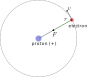
\includegraphics[scale=0.6]{hydrogenAtom}
	\caption{Planetary model of hydrogen atom.}
	\label{fig:hydrogenAtom}
\end{figure}

The circular motion of the electron around the nucleus is
mathematically similar to the problem of a planet circling a
star. Using the second law of Newton and the expression for the
Coulomb's force, we can write
\[
\frac{m_ev^2}{r} = k\frac{q_e^2}{r^2}\,,
\]
where
\[
k = \frac{1}{4\pi\varepsilon_0}\,.
\]

Newtonian momentum is given by $p=mv$; from the motion equation
above, we find
\[
p^2 = k\frac{m_e q_e^2}{r}\,.
\]

\begin{figure}[htbp]
	\centering
	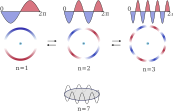
\includegraphics[scale=1.0]{hydrogenAtomOrbits}
	\caption{Orbits allowed by the semi-quantum model.}
	\label{fig:hydrogenAtomOrbits}
\end{figure}

Using de Broglie hypothesis about the relation between momentum and
wavelength
\[
p\lambda = h\,,
\]
and combining it with \emph{quantization hypothesis}:
\[
n\lambda = 2\pi r
\]
or, equivalently,
\[
pr = n\frac{h}{2\pi} = n\hbar\,
\]
we find possible solutions for the radius of the ``orbit'':
\[
r_n = \frac{\hbar^2 n^2}{km_e q_e^2}\qquad n = 1, 2, 3,\ldots
\]
The smallest value of the radius is
\[
a_0 = r_1 = \frac{4\pi\varepsilon_0 \hbar^2}{m_e q_e^2} = 0.523\,\r{A}\,.
\]
It is called \emph{Bohr radius}. Thus, the smallest diameter of
electron's orbit is about 1 \r{A}ngstrom.
\begin{exercise}
	Find the numbers for which the radius of electron ``orbit'' equals:
	1) 1 mm; 2) 1 cm; 3) 1 m.
\end{exercise}

How fast does the electron move around the nucleus? The velocity
of the electron is
\[
v = \sqrt{\frac{kq_e^2}{m_e r}}\,.
\]
Substituting $r_n = a_0 n^2$ we get
\[
v_n = \frac{1}{n}\sqrt{\frac{kq_e^2}{m_e a_0}} = \frac{v_1}{n}\,.
\]
The value of $v_1$ is
\[
v_1 = 2.19\times 10^6\,(m/s)
\]
Although this is a big number, it is much smaller than the speed of
light; we are therefore justified in using Newtonian mechanics and not
taking relativity into account.

\begin{mybio}{Quantization in Astronomy}
	The ``quantization'' of orbit radius can be found even for planets in
	solar system. If we denote the distance between the earth and the sun
	as $A$ (called \emph{astronomical unit}), then the distances to
	planets from the sun are given by the formula
	\[
	r_n = \frac{A}{10}(4+3\times 2^n)\,.
	\]
	This relation is known as \emph{Titius-Bode} law. It works remarkably
	well for all planets from Venus ($n=0$) to Uranus ($n=6$).
\end{mybio}

How strong is the electron attracted to the nucleus? The Coulomb force
between the charges is
\[
F = \frac{kq_e^2}{r^2}\,.
\]
Substituting $r_n = a_0 n^2$ we get
\[
F_n = \frac{kq_e^2}{a_0^2 n^4} = \frac{F_1}{n^4}\,.
\]
The value of $F_1$ is
\[
F_1 = 8.24\times 10^{-8}\,(N)
\]
This is a tiny force on the human scale of forces. Even a baby ant has enough force to tear a hydrogen atom apart with its "bare hands"!

Although the force acting on the electron is small on a human scale,
the acceleration ($a=v^2/r$) it produces is very large (on the human
scale, compare to $g$). This is due to extreme lightness of the
electron:
\[
m_e = 9.1\times 10^{-31}\, (kg)\,.
\]

What is the total energy of the hydrogen atom? It can be found as
follows:
\[
E_n = \frac{m_ev_n^2}{2}-k\frac{q_e^2}{r_n} = -\frac{E_1}{n^2}\,,
\]
where
\[
E_1 = k\frac{q_e^2}{2m_e a_0}\,.
\]
The value of $E_1$ is
\[
E_1 = 2.18\times 10^{-18}\, (J)\,.
\]
In atomic world a special unit of energy is used. It is the energy of
electon accelerated by a voltage drop of 1 Volt:
\[
E_{ev} = 1\,(V)\times q_e = 1.6\times 10^{-19}\, (J)\,.
\]
Using this atomic unit, the hydrogen atom has energy
\[
E_1 = 13.6\, (eV)\,.
\]

\begin{exercise}
	What is the frequency of revolution of electron around the nucleus
	for an orbit number $n$?
\end{exercise}

\subsubsection{Atoms Can't Exist?}
The model described above leads to the conclusion that atoms must not
exist for long. According to the theory of classical electrodynamics,
a charge moving in a circle will emit electromagnetic
waves with the frequency of revolution. As the atom loses its energy,
the electron spirals ever closer to the nucleus. Taking classical
electrodynamics into account, the life-time of a hydrogen atoms should
be about nanosecond. This contradicts the observation of stability of
atoms.

Niels Bohr suggested that the ``orbits'' represent so called
\emph{stationary states}, where electrons can ``move'' without
radiating away electromagnetic waves. Radiation only happens when
electron \emph{transitions} between stationary levels, for example
between 2 and 4. The energy carried away by the light is related to
the frequency of the electromagnetic wave $\nu$ as follows:
\[
\Delta E = E_m - E_n = h\nu_{nm}\qquad m > n\,.
\]

%\begin{tcolorbox}[colback=white!85!ocre, title=Exercise]
\begin{exercise}
	How much energy is required to ``move'' electron from the``orbit''
	of 1 mm to 1 cm? From 1 cm to 1m?
\end{exercise}
%\end{tcolorbox}

\subsubsection{Line Spectra Explained}
Using the results obtained above, we can now describe the spectra of
light emitted or absorbed by hydrogen.

The stationary states are discrete, therefore there are discrete
energies of transition between a pair of levels. When atom absorbs
electromagnetic radiation, electron ``jumps up'' to higher energy
level and farther distance. In the reverse process, electron ``jumps
down'' from higher level to lower one, resulting in emission.

The wavelength of the radiation is
\[
\lambda = cT = \frac{c}{\nu} = \frac{ch}{E_m - E_n}\,.
\]
Plugging in the expression for the energy, we get
\begin{equation}
	\lambda = \frac{ch}{E_1}\frac{n^2m^2}{m^2-n^2} = 91.127(nm)\times\frac{n^2m^2}{m^2-n^2}\,.
	\label{eq:lambdaSeries}
\end{equation}

A special case of this formula was discovered in 1885 by a Swiss
mathematician Johan Balmer. Analyzing the visible lines in the spectra
of hydrogen, he found some regularity in the wavelengths. Balmer
expressed it as follows:
\[
\lambda = B\frac{m^2}{m^2-2^2}\,,
\]
where $m > 2$ and $B=364.51$ nm.
Looking at (\ref{eq:lambdaSeries}), we can see that it can be written
for $n=2$ as
\[
\lambda = 91.127(nm)\times \frac{4m^2}{m^2-2^2} = 364.51(nm)\times \frac{m^2}{m^2-2^2}\,.
\]

%\begin{tcolorbox}[colback=white!85!ocre, title=Exercise]
\begin{exercise}
	According to the the formula  (\ref{eq:lambdaSeries}), how many
	hydrogen lines will be in the visible part of the spectrum (from
	400nm to 700nm)?
\end{exercise}
%\end{tcolorbox}

\begin{mybio}{Three Body Problem}
	The problem of hydrogen atom involves \emph{three} physical entities
	interacting with each other: Proton, electron, and electromagnetic
	field. Electron does not interact directly with the proton, it does
	so via the electric field of the nucleus. This is important to keep
	in mind, especially if we want to understand the phenomenon of
	\emph{spontaneous emission}.
\end{mybio}

\subsection{Landau Levels and Magnetic Flux Quantization*}
The simple semi-classical approach to quantization used for hydrogen atom can be applied to another interesting quantum effect appearing when electrons are moving in a strong magnetic field.

\[
qvB = \frac{mv^2}{r}\,\to\, qBr=mv
\]

\[
qBr^2 = mvr = n\hbar\,.
\]
Thus, the radius can only be $r_n=r_1\sqrt{n}$ where $r_1=\sqrt{\hbar/qB}$. Kinetic energy is $E_n = E_1 n$ where
$E_1 = q\hbar B/2m$.

The quantity $\Phi=\pi r^2 B$ is called \emph{magnetic flux} -- a measure of the "flow" of magnetic field $B$ throught the area $\pi r^2$. In terms of magnetic flux, the quantization condition becomes
\[
\Phi = n\Phi_0\,,
\]
where $\Phi_0=h/2e$ is known as \emph{elementary magnetic flux quantum}. It is the smallest step magnetic flux can change by.


\subsubsection{Spontaneous Emission and Cavity QED}
According to Schrodinger equation, an hydrogen atom with electron in any
statioary state $\qs{\Psi_n}$ with energy $E_n$ will remain in this
state \emph{forever}. In reality, every atom will randomly transition
into a state with lower energy, all the way to the lowest energy
state, emitting radiation as the result. This is called \emph{spontaneous
	emission}.

To describe spontaneous emission, one must account for the fact that
atom is not truly isolated and electron and proton are not the only
quantum systems in picture. There is an electromagnetic field with its
many modes-oscillators.

Interaction of atom-like quantum systems (qubits, quantum dots, atoms)
with quantum states of electromagnetic field is the focus of an exctiting
area of research called \emph{Cavity Quantum Electrodynamics} or \emph{cavity QED} (CQED).
\begin{figure}[htbp]
	\centering
	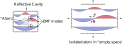
\includegraphics[scale=1.0]{cavityQED}
	\caption{Atom in ``empty space'' is a quantum system in a very large
		cavity, coupled to the modes-oscillators of electromagnetic field.}
	\label{fig:cavityQED}
\end{figure}

\subsection{Franck-Hertz Experiment}
Atoms can transition between different states by absorbing energy from electromagnetic radiation ("photons").  But this is not the only mechanism. Other particles, like electrons, can transfer their kinetic energy to atoms by bumping into the latter. Such a phenomenon was studied by James Franck and Gustav Hertz in 1914 using collisions of electrons with mercury atoms enclosed in a special vacuum tube. They showed that whenever electrons had a certain kinetic energy -- specific to mercury atoms -- they transfered this energy very efficiently (\emph{resonantly}) to mercury atoms. When the energies of electrons and mercury atoms were not matched, electrons scattered from the atoms \emph{elastically} -- without the loss of their kinetic energy.  The work of Franck and Hertz was recognized with 1925 Nobel Prize in Physics. Interestingly, according to James Franck, neither he nor Gustav Hertz had any knowledge of Bohr's theory of atomic states when they performed their experiment.

\subsubsection*{Idea}
The idea of Franck-Hertz experiment is illustrated in figure \ref{fig:franckHertzExperiment}. Its central part consists of a closed vacuum tube with mercury gas and several electric elements used as the source and sink of electrons.
\begin{figure}[htbp]
	\centering
	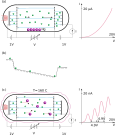
\includegraphics[scale=1.0]{franckHertzExperiment}
	\caption{(a) A vacuum tube is used to study the flow of electrons between two metal electrods under various conditions.; (b); (c).}
	\label{fig:franckHertzExperiment}
\end{figure}


\subsubsection*{Numbers}
At room temperature mercury is a liquid metal which can be easily turned into a gas by heating it up to 200$^\circ$C. Unlike molecular gases such as hydrogen $H_2$, oxygen $O_2$, or nitrogen $N_2$, \emph{mercury gas is monoatomic} -- consisting of single $Hg$ atoms.

Each mercury atom contains 80 protons and 120 neutrons and is significantly heavier than an electron: $M_{Hg}\approx 4\times 10^5\,m_e$.  Consequently, an electron colliding with a mercury atom won't be able to impart any appreciable recoil speed. In other words, mercury atoms are like immovable objects to electrons.  
\begin{exercise}
	Show that for the head-on collision the speed of an initially stationary mercury atom after the collision becomes $v=2v_0\frac{m_e}{M_{Hg}}$.
\end{exercise}

\subsection{Stoke's Rule}
Stoke's rule.

\section{Rydberg Atoms}
When an atom has outer electron(s) excited into states with high excitation number  $n$, it is called a \emph{Rydberg atom}(CHECK!). Such atoms are of great importance for experiments of quantum physics.

\section{Quantum Dots}
Quantum dots are physical structures designed to confine electrons in tiny volumes. They are human-made and can be viewed as \emph{artificial atoms}. As the result of confinement, quantum states of the trapped electrons form a discrete set not unlike the states of a hydrogen atom. \emph{Examples:???}

To illustrate the idea, consider an idealized case of an electron confined in one dimension in a region between $x=0$ and $x=L$.

\[
\ketbra{\alpha}{\beta}
\]
\[
E_n = -\frac{E_i}{n^2}\,.
\]

\section{Spontaneous Emission}
When an excited atom is left alone, it must remain in the excited state \emph{forever}. This follows from the Schrodinger's equation:
\[
i\hbar \partial_t\,\ket{\psi}=\op{H}\ket{\psi}
\]
If $\op{H}\ket{\psi}=E_n\ket{\psi}$ we get
\[
\partial_t\,\ket{\psi}=\beta\ket{\psi}\,,\textrm{ where } \beta = \frac{-iE_n}{\hbar}\,.
\]
The solution to this equation is 
\[
\ket{\psi_t} = e^{\beta t}\ket{\psi_0}=e^{-iE_n/\hbar}\ket{n}\,.
\]

However, atoms placed in the best isolation allowed by an experiment, inevitably transition to the lowest (ground) energy state, emitting energy in the form of EMF excitation. The process is random and resembles a radioactive decay.

\section{Stimulated Emission}
\[
\ketbra{\alpha}{\beta}
\]
\[
E_n = -\frac{E_i}{n^2}\,.
\]

\section{Lasers}
Laser is a device that produces a special kind of light --\emph{monochromatic} and  \emph{coherent} electromagnetic radiation.
Monochromatic means "single color" or single wavelength. Coherent means capable of interference, which implies stable \emph{phase}.

 Laser can be described on several levels: classical, semiclassical, and quantum.

Any laser has three main components: 
\begin{enumerate}
	\item \emph{Cavity} to create mode.
	\item \emph{Gain medium} to amplify signal.
	\item \emph{Pump} to keep energy flowing into the gain medium.
\end{enumerate}

From the standpoint of quantum physics, lasers are special \emph{sources of excitation of electromagnetic field}. Laser's operation is based on the effect of {\bf L}ight {\bf A}mplification by the {\bf S}timulated {\bf E}mission of {\bf R}adiation (LASER).
\[
\ketbra{\alpha}{\beta}
\]
\[
E_n = -\frac{E_i}{n^2}\,.
\]


\begin{figure}[htbp]
	\centering
	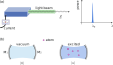
\includegraphics[scale=1.0]{laser}
	\caption{(a); (b)}
	\label{fig:laser}
\end{figure}



\section{Photoeffect}
The phenomena related to photoelectric effect, or photoeffect, are so important that three separate Nobel prizes have been awarded to people who contributed to their discovery, explanation, and confirmation. 
\begin{mybio}{Noberl Prizes for Photoeffect}
	The first Nobel prize was given to Philipp Eduard Anton von Lenard in 1905 for {\it "for his work on cathode rays"} (CHECK DETAILS!). The second Nobel prize was awarded to Albert Einstein in 1921 {\it "for his services to Theoretical Physics, and especially for his discovery of the law of the photoelectric effect"}. The third Nobel prize was awarded to Robert Millikan in 1923 for {\it "for his work on the elementary charge of electricity and on the photoelectric effect"}.
\end{mybio}
An EMF excitation -- a photon -- with frequency $\nu$ and energy $E=h\nu$ can impart its energy to an electron bound inside a material (e.g. metal). If the energy is sufficient to free the electron, it can escape with the kinetic energy
\[
E = h\nu - W\,,
\]
where $W$ is the energy which a \emph{free electron} needs to move outside of a material. $W$ is called a \emph{work function} and it is a number specific to a material. 


\[
\ketbra{\alpha}{\beta}
\]
\[
E_n = -\frac{E_i}{n^2}\,.
\]

\section{Black Body Radiation}
\[
\rho_\nu = \frac{2h\nu^3}{c^2}\frac{1}{e^{h\nu/kT}-1}\,.
\]
\[
E_n = -\frac{E_i}{n^2}\,.
\]

\section{Conductors}
\[
\ketbra{\alpha}{\beta}
\]
\[
E_n = -\frac{E_i}{n^2}\,.
\]

\subsection{Heat Capacity}
Einstein's model.

\section{Entanglement}
Entanglement can be viewed as a \emph{physical resource} of purely quantum nature. As a resource, entanglement facilitates several important processes related to processing of information.
\[
\ketbra{\alpha}{\beta}
\]
\[
E_n = -\frac{E_i}{n^2}\,.
\]
\subsection{Teleportation}
In quantum physics \emph{teleportation} means a "transfer" of a quantum state to a distant location. 
In the process of teleportation the original quantum state is "erased" in one place and "reconstructed" at a target location.

It important to understand that quantum teleportation does not imply sending \emph{objects}, \emph{energy}, or a \emph{signal} instanteneously from one place to another. Quantum teleportation has nothing to do with the popular sci-fi notion of object teleportation.

\subsection{Entanglement And Measurement}
Entanglement -- a purely quantum effect -- plays the central role in the measurement process.


\section*{Chapter Highlights}
{\setstretch{1.5}\chhc
  \it
\begin{itemize}
\item Tensors find application in various areas of science and math.
\item Geometrical properties of surfaces and spaces can be described
  using metric tensor.
\item Physical properties of solids are often anisotropic -- depend on
  the direction of applied ``force''. Such properties are best
  described by various tensors: stress tensor, mobility tensor,
  piezoelectric tensor, and others.
\item At the fundamental level electric and magnetic fields are united
  in a single physical object -- electromagnetic field. Electromagnetic
  field is described by an antisymmetric tensor of the second rank.
\end{itemize}

}


\chapterimage{pics/chapterImageDefault.pdf}
%% %\chapterimage{relativity.pdf}
\graphicspath{{../07Implications/pics/}}

\chapter{Implications}\label{ch:Implications}

\lettrine[lines=2]{\color{darkocre}W}{e} are now ready to appreciate
the implications of quantum physics.

\begin{myprereq}{Prerequisite Knowledge}
	To fully understand the material of this chapter, readers should be comfortable with the following concepts:
	
	\begin{itemize}
		\item \phantom{phantom}
		\vspace{-0.5cm}
		\item State
		\item Dynamical equations
	\end{itemize}	
\end{myprereq}


Discuss Mermins papers. Wheeler's ideas.

\subsubsection*{$\delta$-Notation}\index{Notation!delta}
When a quantity $x$ changes by a tiny amount, we will denote the
change using small Greek letter $\delta$ (delta) as follows:
\[
\colorboxed{blue}{\delta x\textrm{ - tiny change of } x.}
\]
A convenient way to write all components of a second rank tensor is to
use table-like structure called \emph{matrix}.

\section*{Chapter Highlights}
{\setstretch{1.5}\chhc
	\it	
	\begin{itemize}
		\item Tensors find application in various areas of science and math.
		\item Geometrical properties of surfaces and spaces can be described
		using metric tensor.
		\item Physical properties of solids are often anisotropic -- depend on
		the direction of applied ``force''. Such properties are best
		described by various tensors: stress tensor, mobility tensor,
		piezoelectric tensor, and others.
		\item At the fundamental level electric and magnetic fields are united
		in a single physical object -- electromagnetic field. Electromagnetic
		field is described by an antisymmetric tensor of the second rank.
	\end{itemize}
	
}

\chapterimage{pics/chapterImageDefault.pdf}
%% %\chapterimage{relativity.pdf}
\graphicspath{{../08Appendix/pics/}}


\chapter{Appendix}\label{ch:Appendix}

\lettrine[lines=2]{\color{darkocre}W}{e} are now ready to appreciate
the implications of quantum physics.

\section{Physics}
When a quantity $x$ changes by a tiny amount, we will denote the
change using small Greek letter $\delta$ (delta) as follows:
\[
\colorboxed{blue}{\delta x\textrm{ - tiny change of } x.}
\]
A convenient way to write all components of a second rank tensor is to
use table-like structure called \emph{matrix}.
\subsection{Black Body Radiation}

\subsection{Notation}
$K$ and $E_k$ -- Kinetic energy of a system.\\
$\Pi$ and $E_p$ -- Potential energy of a system.\\
$E$ -- Total mechanical energy ($E=E_K+E_P$) written in terms of velocity $v$ and position $x$.\\
$H$ -- Hamiltonian of a system: $H=K+\Pi$. Differs from $E$ because
kinetic energy written in terms of \emph{momentum} $p$ instead of velocity.\\
$L$ -- Lagrangian (Lagrange function) of a system: $L=E_K-E_p$. It is the ``imbalance''
of energies.\\
$\Delta x$ -- Change of a value of a variable $x$.\\
$\delta x$ -- ``Tiny'' change of a value of a variable $x$.\\
$\partial$ -- Rate of change.\\
$\partial_{t}$ -- Rate of change with respect to time.\\
$\partial_{x}$ -- Rate of change with respect to variable $x$
(e.g. position).\\
$\partial_{t}f$ -- Rate of change of $f$ with respect to $t$.\\
It means exactly the following
\[
\partial_t f = \frac{\delta f}{\delta t}=\frac{f(t+\delta t)-f(t)}{\delta t}\,.
\]\\
$\vec{\xi}$ -- State of a system in Hamiltonian dynamics. It is a vector
with components $\vec{\xi}=(x,p)$.\\
$\hat{J}$-- Operation (operator) of rotation by 90 degrees.\\
$\hat{R}(\theta)$ -- Operation (operator) of rotation by $\theta$.\\
$h$ -- Quantum of action (Planck's constant). In SI units its numerical
value is $h=6.626\times10^{-34}(J\cdot s)$.\\
$\hbar$ -- ``Reduced Planck's constant''. A convenience notation
for often used combination $\hbar=h/(2\pi)$.\\
$A$ -- Action.\\
$\Psi$ -- Quantum state.\\
$|\Psi\rangle$ -- Quantum state vector.\\
$\phi,\,\theta$ -- Angle variables.\\
$\omega$ -- Angular speed (also angular velocity). Often it has
the following meaning: $\omega=\partial_{t}\theta$ .\\
$\vec{e_{1}},\vec{e_{2}}$ -- Basis vectors. Usually they have unit
length and point in mutually perpendicular directions.\\
$z$ -- Arbitrary \emph{numeric} variable, $\vec{z}$ -- arbitrary
\emph{vector} variable, $\hat{z}$ -- arbitrary \emph{operator}.\\
$\overset{\circ}{A}$ -- Angstrom, a unit of length in the world
of atoms. $1\overset{\circ}{A}=10^{-9}(m)$. Hydrogen atom is about
$1\overset{\circ}{A}$ in diameter.\\
$c$ -- Speed of light in vacuum.\\
$\nu$ -- Frequency of oscillations measured as the number of
oscillations per second, in Hz.


\subsection{Physical Constants}
Below is the list of various physical constants used in these notes.\\
$q_e = 1.6\times 10^{-19}\,(C)$ -- Charge quantum (charge of an
electron).\\
$m_e = 9.1\times 10^{-31}\,(kg)$ -- rest-energy (aka mass) of an electron.\\
$k=\frac{1}{4\pi\epsilon_0} = 9\times 10^9\,(N\cdot m^2/C^2)$ --
Coulomb constant -- force between two unit charges 1 meter apart.\\
$10^{-9}$ s = 1 nanosecond -- the unit of time in atomic world. It is a ``heartbeat
of atoms''.\\
$1\, (eV) = q_e\, (J)$ -- 1 electron-volt. It is the kinetic energy
an electron would acquire when accelerated by a simply 1V battery. A
tiny value.\\
$m_ec^2/q_e= 0.5\, MeV$ -- rest-energy of an electron measured in
electron-volts. Roughly speaking, we will need half a million
1-volt batteries to accelerate an electron to make its kinetic energy
comparable to its rest-energy. \\
$k=100\,(N/m)$ is a spring constant of a spring that stretches by 0.1
of a meter when 1 kilogram mass is attached to it.\\



\section{Mathematics}
When a quantity $x$ changes by a tiny amount, we will denote the
change using small Greek letter $\delta$ (delta) as follows:
\[
\colorboxed{green}{\delta x\textrm{ - tiny change of } x.}
\]
A convenient way to write all components of a second rank tensor is to
use table-like structure called \emph{matrix}.

\subsection{Greek Alphabet}
\begin{table}[h]
  \begin{tabular}{l l c l l}
    \toprule
    $\mathrm{A}\, \alpha$ & alpha & & $\mathrm{B}\, \beta$ & beta\\
    $\Gamma\, \gamma$ & gamma & & $\Delta\, \delta$ & delta\\
    $\mathrm{E}\, \epsilon$ & epsilon & & $\mathrm{Z}\, \zeta$ & zeta\\
    $\mathrm{H}\, \eta$ & eta & & $\Theta\, \theta$ & theta\\
    $\mathrm{I}\, \iota$ & iota & & $\mathrm{K}\, \kappa$ & kappa\\
    $\Lambda\, \lambda$ & lambda & & $\mathrm{M}\, \mu$ & mu\\
    $\mathrm{N}\, \nu$ & nu & & $\Xi\, \xi$ & xi\\
    $\mathrm{O}\, \mathrm{o}$ & omicron & & $\Pi\, \pi$ & pi\\
    $\mathrm{P}\, \rho$ & rho & & $\Sigma\, \sigma$ & sigma\\
    $\mathrm{T}\, \tau$ & tau & & $\Upsilon\, \upsilon$ & upsilon\\
    $\Phi\, \phi$ & phi & & $\mathrm{X}\, \chi$ & chi\\
    $\Psi\, \psi$ & psi & & $\Omega\, \omega$ & omega\\
    \bottomrule
  \end{tabular}
  \caption{Greek Alphabet}
\end{table}

In mathematics most often we use $\theta$ and $\phi$ for
angles. Sometimes $\alpha$ and $\beta$ are also used. Occasionally
$\psi$ is used to denote angle.

In physics $\lambda$ is used to denote the wavelength of light, $\nu$
-- frequency in Hertz (periods of oscillations per second), $\omega$
-- angular speed (number of radians of rotation per second).

The symbols $\Psi$ and $\Phi$ are usually used to denote quantum state vectors.


\subsection{Available Environments}
Coloredboxed environment, with \textbackslash coloredboxed\{color\}\{ text \}:
\[
\colorboxed{red}{E=mc^2}.
\]

Bold text command inside math mode is \textbackslash btc\{ txt\}:

\[
\btc{max}\,x\,y
\]

Bold text with emphasis (italic) is done with \textbackslash bem\{text\}:
\bem{example of a very important piece of text}.



Grey bullet: \textbackslash tus:
\tus\tus\tus\tus

Quantum state is \textbackslash qs: $\qs{\psi}$ or better use ket and bra commands: $\ket{\phi}$ and $\bra{\psi}$.

Bracket and ketbra combinations using a single command: $\braket{\psi}{\phi}$ and $\ketbra{\psi}{\phi}$.

Operators are set with \textbackslash op\{name\}:
$\op{\rho}=\ketbra{\psi}{\psi}$.

\[
\oop{\rho} \ne \op{\rho}
\]

\subsubsection{Environments}

Prerequisite environment \textbackslash myprereq\{text\}:
\begin{myprereq}{Prerequisites}
	One, two, and three.
\end{myprereq}


Example environment \textbackslash myExample\{text\}:
\begin{myExample}
	This is a perfect example.
\end{myExample}

Analogy environment \textbackslash analogy\{text\}:
\begin{analogy}
	Consider the following analogy: A and B.
\end{analogy}

Definition environment \textbackslash mydef\{text\}:
\begin{mydef}{Kinetic Energy}
	Kinetic energy is the energy due to motion.
\end{mydef}

Reminder environment \textbackslash myrem\{text\}:
\begin{myrem}{Kinetic Energy}
	Recall that $E_k=mv^2/2$.
\end{myrem}

Bio environment \textbackslash mybio\{text\}:
\begin{mybio}{Max Planck}
	The full name of Max Planck is Max Karl Ernst Ludwig Planck.
\end{mybio}

\section{Temporary Stuff}
Work in progress sections will be kep here.

\subsection{Facts About Light}
Our understanding of the physical nature of light is the result of several centuries of studies. Visible, infra-red or ultra-violet  light, and microwave or gamma radiation are all various manifestations of \emph{electro-magnetic field} (EMF). It is one of the most technologically important and well-understood fields. 

\subsubsection*{Omnipresence}
The first important fact about EMF is that it is truly ubiqutous: There is no place in the universe free from EMF. Yes, there are regions of space (and time) where EMF is not excited, but EMF is still present there in its "unexcited" form, called \emph{EMF-vacuum}. This vacuum state is an important quantum state of EMF. It is discussed in more details in Section XXX.

\subsubsection*{Localizability}
The second important fact about EMF is its ability to be localized (concentrated) in finite regions of space, simetimes in small volumes. Put differently, EMF can be excited ("emitted") by relatively small "objects" (sources of EMF excitations) or absorbed by similar objects. Emission and absorption of light by atoms is a perfect example of this principle.

\begin{myrem}{Localized Excitations}
	We must clarify: It is the \emph{excitation of EMF} which is localized, \emph{not} EMF. The latter is everywhere, always.
\end{myrem}


\subsubsection*{Energy-Momentum}
Excitations of EMF propagate through space and possess the basic mechanical aspect -- \emph{energy-momentum}. When an atom emits a pulse of light it loses certain energy when and it also experiences a recoil, like a gun that fires a bullet. An EMF excitation carrying energy $E$ also carries momentum $p$. The two are related as follows:
\[
E = pc\,,
\]
where $c$ is the speed of light -- the speed of propagation of EMF through "empy" space. This formula is a special case of a more general relation between energy and momentum, derived in the special theory of relativity:
\[
E^2 = p^2 c^2 + m^2c^4\,.
\]
This is the relation between \emph{total} (kinetic and non-kinetic) energy of an object with mass $m$ and momentum $p$. It shows that even for an object at rest ($p=0$) it still possesses non-kinetic energy -- called rest-energy -- equal $E_0=mc^2$. For EMF excitations the total energy $E$ is \emph{purely due to motion} or, equivalently, EMF excitations are massless $m=0$.
\begin{myrem}{Photons}
	In common language, propagating EMF excitations are called \emph{photons}. It is sometimes said that photons with energy $E$ carry momentum $p=E/c$ and that photons are massless particles. It must be emphasized again that such language is not always helpful.
\end{myrem}

\subsubsection*{Colors}
Beyond energy-momentum, EMF excitations exhibit various "colors" -- both visible and invisible to the human eye.

\subsubsection*{Timeless Law}
The laws that describe the behavior of electromagnetic radition in space and time are expressed by the equations which show no preference to the direction of time flow.



\chapterimage{pics/chapterImageDefault.pdf}
%% %\chapterimage{relativity.pdf}
\graphicspath{{../09Solutions/pics/}}

\chapter{Solutions}\label{ch:Solutions}
%\small
\footnotesize

\subsubsection*{Exercise \ref{exe:carMakesSet}}

\begin{figure}[htbp]
  \centering
  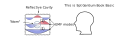
\includegraphics[scale=1.0]{defaultFigureTemplate}
  \caption{The set $M$ contains all possible makes of cars: Ford,
    Toyota, etc.}
  \label{fig:diagramCars}
\end{figure}

The diagram in the Figure \ref{fig:diagramCars} shows the set $M$ -- the set
of all possible makes of cars. A mapping $\btc{trk}$ returns $true$ if a
given car maker produces trucks.

\subsubsection*{Exercise \ref{exe:relationsGeneral}}
\begin{figure}[htbp]
  \centering
  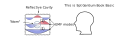
\includegraphics[scale=1.0]{defaultFigureTemplate}
  \caption{(a) Two inputs (outputs) of a function can be replaced with
    a single input of a \bem{pair} of numbers, turning a binary
    function into a unary one. (b) That.}
  \label{fig:diagramProductSet}
\end{figure}

Any binary function can be viewed as a unary function
if two inputs are replaced by a single input of a \emph{pair of
numbers}. Similarly for a function with two outputs. This idea is
illustrated in the Figure \ref{fig:diagramProductSet}(a): The function
{\bf swp} is viewed as a unary function which swaps the numbers in an
\emph{ordered pair}:
\[
\textbf{ swp }\,(n,m) = (m, n)\,.
\]

Given the set $\mathbb{Z}$ of whole numbers, we can create the set of
all possible \emph{ordered pairs} $(n,m)$. This set can be denoted as
follows:
\[
(\mathbb{Z}, \mathbb{Z})\,\textrm{ or }\, \mathbb{Z}\times\mathbb{Z}\,.
\]

The latter notation is standard in mathematics, but the former way
of writing is also acceptable. We can similarly denote the set of all
\emph{ordered triples}:
\[
(\mathbb{Z}, \mathbb{Z}, \mathbb{Z})\,\textrm{ or }\, \mathbb{Z}\times\mathbb{Z}\times\mathbb{Z}\,.
\]

With the notation introduced above, the action of functions with
multiple inputs or outputs can be depicted on the level of sets. The
 Figure \ref{fig:diagramProductSet}(b) shows how this works for the
 functions $\textbf{ swp }$ and $\textbf{ max }$.




%----------------------------------------------------------------------------------------
%	BIBLIOGRAPHY
%----------------------------------------------------------------------------------------

%% \chapter*{Bibliography}
%% \addcontentsline{toc}{chapter}{\textcolor{ocre}{Bibliography}}
%% \section*{Books}
%% \addcontentsline{toc}{section}{Books}
%% \printbibliography[heading=bibempty,type=book]
%% \section*{Articles}
%% \addcontentsline{toc}{section}{Articles}
%% \printbibliography[heading=bibempty,type=article]

%% \cleardoublepage
%% \phantomsection
%% \section*{About Author}

\begin{minipage}{0.3\textwidth}
\includegraphics[scale=0.5]{Pictures/yuryd}
\end{minipage}
\begin{minipage}{0.6\textwidth}\raggedright
Yury Deshko is an American applied physicist, educator, and writer.
He is the author of textbook \emph{``Special Relativity For Inquiring Minds''}
aimed at undergraduate students and motivated
high-schoolers.

When not doing applied physics in silicon photonics,
he develops and teaches modern physics courses (Special Relativity and
Quantum Physics) in summer schools for young aspiring physicists.
\end{minipage}
\noindent
\\

%----------------------------------------------------------------------------------------
%	INDEX
%----------------------------------------------------------------------------------------

\cleardoublepage
\phantomsection
\setlength{\columnsep}{0.75cm}
\addcontentsline{toc}{chapter}{\textcolor{ocre}{Index}}
\printindex

%----------------------------------------------------------------------------------------
%% %  back cover
%% \begingroup
%% \thispagestyle{empty}
%% \begin{tikzpicture}[remember picture,overlay]
%% \coordinate [below=0cm] (midpoint) at (current page.north);
%% \node at (current page.north west)
%% {\begin{tikzpicture}[remember picture,overlay]
%% \node[anchor=north west,inner sep=0pt] at (0,0) {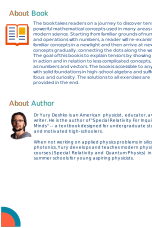
\includegraphics[width=\paperwidth]{Pictures/bookCoverBack_Var1}}; % Background image
%% %\draw[anchor=north] (midpoint) node [fill=ocre!30!white,fill opacity=0.6,text opacity=1,inner sep=1cm]{\Huge\centering\bfseries\sffamily\parbox[c][][t]{\paperwidth}{\centering Relativity\\[15pt] % Book title
%% %{\Large For the Inquiring Mind}\\[20pt] % Subtitle
%% %{\huge Dr. Yury Deshko}}}; % Author name
%% \end{tikzpicture}};
%% \end{tikzpicture}
%% \vfill
%% \endgroup

\end{document}

%%% Local Variables:
%%% mode: latex
%%% TeX-master: t
%%% End:
